%--------------------------------------------------------%
% Journal Article Manuscript Template
%--------------------------------------------------------%

%--------------------------------------------------------%
% DOCUMENT CLASS
%--------------------------------------------------------%

  % Change "letterpaper" to "a4" if you use a4 paper size
  \documentclass[letterpaper,12pt]{article}

%--------------------------------------------------------%
% TITLE SECTION
%--------------------------------------------------------%

  %Abstract
  \usepackage{abstract} % Allows abstract customization
  % Set the "Abstract" text to bold
  \renewcommand{\abstractnamefont}{\normalfont\bfseries}
  % Set the abstract itself to small italic text
  \renewcommand{\abstracttextfont}{\normalfont\small\itshape}

  %Title
  \usepackage{titlesec} % Allows customization of titles

  %Authors
  \usepackage{authblk} % For multiple authors

  %Date
  \usepackage{datetime} % allows for including today's date
  % These two lines creates a new date format ``Month day(th), year''
  \newdateformat{usvardate}{
  \monthname[\THEMONTH] \ordinal{DAY}, \THEYEAR}

%--------------------------------------------------------%
% HEADERS & FOOTERS
%--------------------------------------------------------%

  %Footnotes
  % \usepackage[bottom]{footmisc} % Makes footnotes stick to bottom of the page

  %Headers from page 2 on
  % \usepackage{fancyhdr}
  \pagestyle{plain}
  % \fancyheadoffset{0cm}
%   \setlength{\headheight}{15pt}

%--------------------------------------------------------%
% MACROS
%--------------------------------------------------------%

  % Define keywords macro command
  \providecommand{\keywords}[1]{\textbf{\textit{Keywords---}} #1}

%--------------------------------------------------------%
% MATH SUPPORT
%--------------------------------------------------------%

  % The amssymb package provides various useful mathematical symbols
  \usepackage{amssymb}
  % The amsthm package provides extended theorem environments
  \usepackage{amsthm}
  % The newtxmath package provides additional math symbol support
  % in Times New Roman symbols, etc.
  \usepackage{newtxmath}
  \usepackage{mathtools}
  \usepackage{blkarray, bigstrut}

%--------------------------------------------------------%
% FONTS
%--------------------------------------------------------%

  \usepackage{microtype} % Slightly tweak font spacing for aesthetics
  \usepackage[utf8]{inputenc}
  \usepackage{newtxtext} % Makes default font Adobe Times New Roman

%--------------------------------------------------------%
% LINES
%--------------------------------------------------------%

  % Spacing
  \usepackage{setspace} % See \doublespacing command at the top of content.tex
  % Numbering
  \usepackage{lineno} 	% See \linenumbers at the top of content.tex
  \usepackage[table,x11names]{xcolor}
  % Lists
  \usepackage{enumitem}
  \setlist{nosep}
  \setlist[itemize]{leftmargin=*}

%--------------------------------------------------------%
% MARGINS
%--------------------------------------------------------%

  %NOTE: All spaces in this template are in inches, because it is
  % formatted for letterpaper (8.5 x 11 inch) paper. If you use a4
  % paper, choose different sizes in millimeters or centimeters.
  \usepackage[top=1.5in, bottom=1.5in, left=1in, right=1in]{geometry}

%--------------------------------------------------------%
% COMMENTS
%--------------------------------------------------------%

  \usepackage[colorinlistoftodos]{todonotes} % allows margin comments
  % See examples in content.tex, and here for manual:
  % http://www.ctan.org/pkg/todonotes
  \usepackage{soul} % allows for highlighting


%--------------------------------------------------------%
% ACRONYMS
%--------------------------------------------------------%

  \usepackage[nohyperlinks,nolist]{acronym} % Managing acronyms

%--------------------------------------------------------%
% GRAPHICS
%--------------------------------------------------------%

  \usepackage{graphicx,caption} % More advanced figure inclusion
  \graphicspath{{figures/}} % Set the default folder for images
  \usepackage{float} % For specifying table/figure locations, i.e. [ht!]

  % The printlen command allows the user to print the exact text width or height.
  % This is useful, when trying to create graphics (outside of LaTeX, of course)
  % with the optimal dimensions. See here for usage: http://www.ctan.org/pkg/printlen
  \usepackage{printlen}

  \usepackage[section]{placeins} % Used to ensure that figures do not go into the next section

%--------------------------------------------------------%
% TABLES
%--------------------------------------------------------%

  \usepackage{longtable} % For long tables that span multiple pages
  \newcommand{\sym}[1]{\rlap{#1}}% For symbols like *** in tables
  \usepackage{tabularx} % Allows advanced table features
  \newcolumntype{L}[1]{>{\raggedright\arraybackslash}p{#1}}
  \newcolumntype{C}[1]{>{\centering\arraybackslash}p{#1}}
  \newcolumntype{R}[1]{>{\raggedleft\arraybackslash}p{#1}}
  \usepackage{relsize} % Allows precise adjustment of font size,
  %useful for fitting tables to page width
  \usepackage{multirow}
  %for horizontal tables
  \usepackage{lscape}

%--------------------------------------------------------%
% REFERENCES
%--------------------------------------------------------%

  \usepackage{hyperref} % For hyperlinks in the PDF
  \usepackage{csquotes}
  \usepackage[style=nature,url=false,backend=biber,sorting=none]{biblatex}
  \bibliography{references.bib}

% Header from Page Three on: Edit below for left and right headers
% \lhead{}
% \rhead{}

%--------------------------------------------------------%
% BEGIN DOCUMENT
%--------------------------------------------------------%

\begin{document}

% COVER PAGE

\begin{titlepage}

  \newcommand{\HRule}{\rule{\linewidth}{0.5mm}} % Defines a new command for the horizontal lines, change thickness here

  \center % Center everything on the page


% HEADING SECTION

  %\textsc{\LARGE University Name}\\[1.5cm] % Name of your university/college
  % \textsc{\Large Manuscript Submission}\\[0.5cm] % Major heading such as course name
  % \textsc{\large The Journal of Blah Blah}\\[0.5cm] % Minor heading such as course title

% TITLE SECTION

  \vspace*{\fill}
  {\huge Inferring microbial co-occurrence networks from amplicon data: a systematic evaluation}\\[0.4cm]
  % {\huge  2. Investigating the best practices for inference of microbial co-occurrence networks from 16S data}\\[0.4cm] % Title of your document
  % {\huge  3. Attempting to find the best practice pipeline for inferring co-occurrence networks from 16S data}\\[0.4cm] % Title of your document
  % {\huge  4. Deciphering the complexities in co-occurrence network inference from 16S data}\\[0.4cm] % Title of your document

% AUTHOR SECTION

  \vspace{1.5 cm}
  Dileep Kishore\textsuperscript{a,b},
  Gabriel Birzu\textsuperscript{c,f},
  Zhenjun Hu\textsuperscript{a},
  Charles DeLisi\textsuperscript{a,c},
  Kirill S. Korolev\textsuperscript{a,b,c}\#,\\
  Daniel Segr\`{e}\textsuperscript{a,b,d,e}\#\\
  \vspace{1cm}
  \textsuperscript{a}Bioinformatics Program, Boston University, Boston, Massachusetts, USA\\
  \textsuperscript{b}Biological Design Center, Boston University, Boston, Massachusetts, USA\\
  \textsuperscript{c}Department of Physics, Boston University, Boston, Massachusetts, USA\\
  \textsuperscript{d}Department of Biomedical Engineering, Boston University, Boston, Massachusetts, USA\\
  \textsuperscript{e}Department of Biology, Boston University, Boston, Massachusetts, USA\\
  \textsuperscript{f}Department of Applied Physics, Stanford University, Stanford, California, USA\\
  \textsuperscript{$\#$}Correspondence should be sent to \href{mailto:korolev@bu.edu}{korolev@bu.edu} or \href{mailto:dsegre@bu.edu}{dsegre@bu.edu}\\

  \vspace{2cm}

% % DATE SECTION

  % \vspace{1.5 cm}
  % {\large Submitted: \today}\\[3cm] % Date, change the \today to a set date if you want to be precise


  \vspace*{\fill} % Fill the rest of the page with whitespace

\end{titlepage}

%-----------------------------------------------------------------

\newpage

\thispagestyle{empty} % Removes header on page two.

% NOTE: Comment out the lines below to remove line numbers
  % Running line numbers:
  \linenumbers
  \setlength\linenumbersep{15pt}
  \renewcommand\linenumberfont{\normalfont\footnotesize\sffamily\color{gray}}
  %\pagewiselinenumbers % Same, but that reset on every page:
  \modulolinenumbers[1] % Number only every line. Change for fewer.

%--------------------------------------------------------%
%   CONTENT
%--------------------------------------------------------%

% ABSTRACT
\begin{abstract}
  {
    \noindent
    Microbes commonly organize into communities consisting of hundreds of species involved in complex interactions with each other.
    16S ribosomal RNA (16S rRNA) amplicon profiling provides snapshots that reveal the phylogenies and abundance profiles of these microbial communities.
    These snapshots, when collected from multiple samples, can reveal the co-occurrence of microbes, providing a glimpse into the network of associations in these communities.
    However, the inference of networks from 16S data involves numerous steps, each requiring specific tools and parameter choices.
    Moreover, the extent to which these steps affect the final network is still unclear.
    In this study, we perform a meticulous analysis of each step of a pipeline that can convert 16S sequencing data into a network of microbial associations.
    Through this process, we map how different choices of algorithms and parameters affect the co-occurrence network and identify the steps that contribute substantially to the variance.
    We further determine the tools and parameters that generate robust co-occurrence networks and develop consensus network algorithms based on benchmarks with mock and synthetic datasets.
    The Microbial Co-occurrence Network Explorer or \acs{micone} (available at \href{https://github.com/segrelab/MiCoNE}{https://github.com/segrelab/MiCoNE}), follows these default tools and parameters and can help explore the outcome of these combinations of choices on the inferred networks.
    We envisage that this pipeline could be used for integrating multiple datasets, and for generating comparative analyses and consensus networks that can guide our understanding of microbial community assembly in different biomes.
  }
\end{abstract}

% Insert keywords here
\keywords{Microbiome, 16S rRNA, Interaction, Denoising, Taxonomy, Network Inference, Correlations, QIIME2, Co-occurrence, Networks, Consensus algorithm, Pipeline, nextflow}

% \doublespacing

\section*{Importance}
  Mapping the interrelationships between different species in a microbial community is important for understanding and controlling their structure and function.
  The surge in the high-throughput sequencing of microbial communities has led to the creation of thousands of datasets containing information about microbial abundances.
  These abundances can be transformed into co-occurrence networks, providing a glimpse into the associations within microbiomes.
  However, processing these datasets to obtain co-occurrence information relies on several complex steps, each of which involves numerous choices of tools and corresponding parameters.
  These multiple options pose questions about the robustness and uniqueness of the inferred networks.
  In this study, we address this workflow and provide a systematic analysis of how these choices of tools affect the final network, and guidelines on appropriate tool selection for a particular dataset.
  We also develop a consensus network algorithm that helps generate more robust co-occurrence networks based on benchmark synthetic datasets.

\doublespacing

% INTRODUCTION
\section*{Introduction}

Microbial communities are ubiquitous and play an important role in marine and terrestrial environments, urban ecosystems, and human health \cite{lima-mendezDeterminantsCommunityStructure2015a,Thompson2017,royo-llonchCompendium530Metagenomeassembled2021,tedersooFungalBiogeographyGlobal2014,dankoGlobalMetagenomicMap2021,mclellanMicrobiomeUrbanWaters2015,HumanMicrobiomeProjectConsortium2012}.
  These microbial communities, or microbiomes, often comprise several hundreds of different microbial strains interacting with each other and their environment, often through complex metabolic and signaling relationships~\cite{zelezniakMetabolicDependenciesDrive2015,Ghoul2016,coyteUnderstandingCompetitionCooperation2019,DSouza2018}.
  Understanding how these interconnections shape community structure and function is a fundamental challenge in microbial ecology, and has applications in the study of microbial ecosystems across different biomes.
  With the advancement in DNA sequencing technologies~\cite{huNextgenerationSequencingTechnologies2021,buermansNextGenerationSequencing2014,Narihiro2017},  more information can be extracted from these microbial community samples than ever before.
  In particular, high-throughput sequencing, including metagenomic sequencing and sequencing of 16S rRNA gene amplicons (hereafter referred to as 16S data) of microbial communities, can help detect, identify and quantify a large portion of the constitutive microorganisms of a microbiome \cite{ju16SRRNAGene2015,Jovel2016,quinceShotgunMetagenomicsSampling2017,sedlarBioinformaticsStrategiesTaxonomy2017}.
  These advances have led to large-scale data collection efforts involving terrestrial~\cite{Thompson2017,gilbertMeetingReportTerabase2010,tedersooFungalBiogeographyGlobal2014}, marine~\cite{lima-mendezDeterminantsCommunityStructure2015a,royo-llonchCompendium530Metagenomeassembled2021} and human-associated microbiota~\cite{HumanMicrobiomeProjectConsortium2012,proctorIntegrativeHumanMicrobiome2019,Lloyd-Price2016}.

 This wealth of information has the potential to help us understand how communities assemble and operate.
 In particular, a powerful tool for translating microbiome composition data into knowledge is the construction of association (co-occurrence) networks, in which  microbial taxa are represented by nodes, and frequent co-occurrences (or negative co-occurrences) across datasets are encoded as edges between nodes.
 While the relationship between directly measured interactions~\cite{lubbeExometabolomicAnalysisCrossFeeding2017,Jian2020,Hsu2019} and statistically inferred co-occurrence is still poorly understood \cite{Zuniga2017,Rottjers2018}, a significant amount of effort has gone into estimating co-occurrences from large microbiome sequence datasets~\cite{faustMicrobialCooccurrenceRelationships2012,leeCrosskingdomCooccurrenceNetworks2022,faustMicrobialInteractionsNetworks2012a,maEarthMicrobialCooccurrence2020a}.

 The importance of these networks is two-fold: first, they can serve as maps that help identify hubs of keystone species \cite{Menon2018,Rottjers2018}, and the community response to environmental perturbations or underlying host conditions \cite{Gilbert2016}; second, they can serve as a bridge towards building mechanistic models of microbial communities, greatly enhancing our capacity to understand and control them.
 For example, multiple studies have shown the importance of specific microbial associations in the healthy microbiome \cite{Lloyd-Price2016,Wu2016,HumanMicrobiomeProjectConsortium2012} and their role in dysbiosis \cite{Wang2017,Gilbert2016,Belizario2015}.
 In the context of terrestrial biogeochemistry, co-occurrence networks were shown to help understand microbiome assembly \cite{fiererEmbracingUnknownDisentangling2017}, and  the response of microbial communities to environmental perturbations \cite{Jiao2019}.

One of the most frequently used avenues for inferring co-occurrence networks is the parsing and analysis of 16S sequencing data \cite{Rottjers2018,Friedman2012}.
Numerous software tools and pipelines have been developed to analyze 16S sequencing data, with a strong emphasis on the known limitations of this method, including resolution, sequencing depth, compositional nature, sequencing errors, and copy number variations \cite{Bharti2019,pollockMadnessMicrobiomeAttempting2018}.
Popular methods for different phases of the analysis of 16S data include tools for: (i) quality checking and trimming the sequencing reads; (ii) denoising and clustering the trimmed reads \cite{Caporaso2010,Callahan2016,Amir2017}; (iii) assigning taxonomy to the denoised reads \cite{bokulichOptimizingTaxonomicClassification2018}; (iv) processing and transforming the taxonomy count matrices \cite{weissNormalizationMicrobialDifferential2017}; and (v) inferring the co-occurrence network \cite{Watts2018,Kurtz2015,tackmannRapidInferenceDirect2019}.
Different specific algorithms are often aggregated into popular online platforms (like MG-RAST~\cite{keeganMGRASTMetagenomicsService2016}, Qiita~\cite{gonzalezQiitaRapidWebenabled2018}) and software packages (such as \ac{qiime2}~\cite{bolyenReproducibleInteractiveScalable2019}).
The different methods and tools can lead to vastly different inferences of community compositions and co-occurrence networks \cite{Golob2017,Weiss2016}, making it difficult to reliably compare networks across different publications and studies.
 This difference is partially due to the focus of existing platforms on \ac{otu} or \ac{esv} generation and not on the effects of upstream statistical methods on the inferred co-occurrence networks.
 Furthermore, no organized framework currently exists that can systematically analyze and compare each step in the pipeline for processing amplicons into co-occurrence networks.

 In this study, we present a standardized 16S data analysis pipeline called \ac{micone} that produces robust and reproducible co-occurrence networks from 16S sequence data of microbial communities, and enable users to interactively explore how the network would change upon using different alternative tools and parameters at each step.
 Our pipeline is coupled to an online integrative tool for the organization, visualization, and analysis of inter-microbial networks called \ac{mind}~\cite{huResourceComparisonIntegration2022}, which is available at \href{http://microbialnet.org/}{http://microbialnet.org/}.
Through a systematic comparative analysis, we determine which steps of the \ac{micone} pipeline have the largest influence on the final network, and which choice seems to have the optimal agreement with the tested mock and synthetic datasets.
These steps together with our default settings ensure better reproducibility and easier comparison of co-occurrence networks across datasets.
We expect that our tool will also be useful for benchmarking future alternative methods, and for ensuring a transparent evaluation of the possible biases introduced by the use of specific tools.

% RESULTS
\section*{Results}

  \subsection*{\acl{micone} (\acs{micone})}

  We developed \ac{micone}, a flexible and modular pipeline for the inference of co-occurrence networks from 16S data.
  \ac{micone} incorporates various popular, publicly available tools as well as custom Python modules for 16S data analysis and network inference (Methods).
  The different steps that are a part of the \ac{micone} co-occurrence network inference workflow (Figure~\ref{fig:figure1}) can be grouped into five major modules; (i) \ac{sp}; (ii) \ac{dc}; (iii) \ac{ta}; (iv) \ac{op}; and (v) \ac{ni}.
  Each process in the pipeline is implemented through multiple tools (see Methods and Figure~\ref{fig:figure1}).
  The effects of changing any intermediate step of the pipeline can be evaluated in terms of the final network outcome, as well as on any of the intermediate metrics and data outputs.
  The choice of tools and parameters is encoded in a configuration file (with parameters as shown in Tables S2-S6 at \href{https://github.com/segrelab/MiCoNE-pipeline-paper}{https://github.com/segrelab/MiCoNE-pipeline-paper}).
  Through a systematic analysis of tool combinations at each step of the pipeline, we estimated how much the final co-occurrence network depends on the possible choices at each step.

  Our analysis involved two types of data: The first type consisted of 16S sequencing data from samples of human stool microbiomes from a fecal microbiome transplant (FMT) study of autism~\cite{Kang2017}.
  %\todo[noline]{R2.4}
  The second type was a collection of datasets synthetically or artificially created for the specific goal of evaluating computational analysis tools.
  In particular, in order to benchmark each step in \ac{micone}, we used both mock data (labeled mock4, mock12, and mock16) from mockrobiota~\cite{Bokulich2016} and synthetic networks generated using the NorTA~\cite{Kurtz2015} and seqtime~\cite{Rottjers2018} approaches (See Methods).

  \FloatBarrier

  \subsection*{DC: Denoising and clustering methods differ in their identification of sequences that are low in abundance}

  The \ac{dc} step is commonly carried out to generate representative sequences (in the form of the \acs{otu}/\acs{esv} tables) from the demultiplexed and trimmed 16S sequencing data.
  In order to compare the count tables generated by different tools, we processed the 16S sequencing reads (from the FMT study~\cite{Kang2017}) using 5 different methods: open-reference clustering, closed-reference clustering, de novo clustering, \ac{dada2}~\cite{Callahan2016} and Deblur~\cite{Amir2017}.
  The first three methods are from the vsearch plugin from \ac{qiime2}~\cite{bolyenReproducibleInteractiveScalable2019}.
  The closed and open reference methods in this analysis use the \acl{gg}~\cite{DeSantis2006} database for reference sequence alignment.

  A comparison of the different methods was carried out by calculating the mean UniFrac distances across all samples (Figure~\ref{fig:figure2}).
  The analysis was performed using both the weighted UniFrac~\cite{Lozupone2007} (Figure~\ref{fig:figure2}A) distance metric, which takes into account the counts of the representative sequences, and the unweighted UniFrac~\cite{Lozupone2005} (Figure~\ref{fig:figure2}B) distance metric, which gives equal weights to each sequence.

  The first main message emerging from this analysis is that the representative sequences generated by the different methods, with the exception of Deblur, are similar to each other when weighted by their abundance (Figure~\ref{fig:figure2}A).
  A second message is that the different methods differ mainly in the assignment of sequences of lower abundance.
  This can be inferred from the unweighted comparison (Figure~\ref{fig:figure2}B) which shows an increase in dissimilarity between each pair of methods (see additional details in Supplementary and Figure \ref{fig:figure_s2}).

  These comparisons only elucidate the similarity between a pair of methods.
  To determine which tool most accurately recapitulates the reference sequences in the samples, we applied the same pipeline step to process the mock datasets (mock4, mock12, and mock16) and compared the predicted representative sequences with the true sequences and their distribution.
  The results (Figure~\ref{fig:figure2}C and \ref{fig:figure2}D) show that the predicted sequence distributions are overall different from the expected ones.
  The variation across datasets indicates that the datasets themselves play a big role in method performance.
  We note that there is no method that outperforms the rest in all datasets (see Supplementary for an extended discussion).
  Based on being among the top performers on the mock datasets, their de novo error correcting nature and previous independent evaluation~\cite{Nearing2018}, \ac{dada2} and Deblur appear to be the most reliable.
  This is because the open-reference and de novo clustering methods return a much larger number of \ac{otu}s compared to the other pipelines and would affect the accuracy of the network inference step if stringent filtering is not performed.
  %\todo[noline]{R2.6}
  Overall, since \ac{dada2} as compared to Deblur, displays better performance on all the mock datasets on the weighted UniFrac metric, we set this tool as the default for the DC step of the pipeline.
  %\todo[noline]{R2.10}
  However, if comparison across studies that have sequenced different 16S regions is required, closed-reference and open-reference might be a better option.

  After the denoising, the sequences are subject to Chimera Checking (CC).
  The \ac{micone} pipeline supports two different chimera checking methods, ``uchime-denovo"~\cite{bolyenReproducibleInteractiveScalable2019}, and ``remove bimera"~\cite{Callahan2016}.
  We did not notice any notable difference between the two methods (Figure~\ref{fig:figure_s3}), implying that they identify and remove mostly the same set of sequences as chimeras.
  Since the remove bimera method was originally developed in conjunction with dada2 we use this method as the default.
  The DC step thus results in a reduced set of unique sequences, which will be referred to as representative sequences in the subsequent steps.

  \FloatBarrier

  \subsection*{TA: Taxonomy databases vary widely in taxonomy assignments beyond Order level}

  Taxonomy databases are used to assign taxonomic identities to the representative sequences obtained after the DC step.
  The three 16S taxonomic reference databases used in this study are SILVA~\cite{Quast2012}, \ac{gg}~\cite{DeSantis2006} and \ac{ncbi} RefSeq~\cite{Sayers2009} (Methods).
  These databases vary substantially in terms of taxonomy hierarchies, including species names and phylogenetic relationships~\cite{Balvociute2017}.
  Assignment using a particular database also requires a query tool.
  We used the ``Naive Bayes'' classifier from \ac{qiime2} for the \ac{gg} and SILVA databases and the ``BLAST'' tool (included as a \ac{qiime2} plugin) for the \ac{ncbi} database.
  These tools have been well quantified and optimized~\cite{bokulichOptimizingTaxonomicClassification2018}, hence, we made use of the default parameters in our analyses.

  The representative sequences obtained using the default settings of the DC step were used for taxonomic assignment using the three reference databases.
  Figure~\ref{fig:figure3}A depicts a flow diagram that shows how the top 50 representative sequences (sorted by abundance) are assigned a Genus according to the three databases.
  The different databases lead to assignments that qualitatively display similar distributions. However, the assigned Genus compositions also display clear differences, as does the percentage of unassigned representative sequences (pink).
  Some of the differences in Genus composition have a clear explanation, for example, abundant Genera like Bacteroides and Escherichia are assigned to different representative sequences.
  The large percentage of unassigned sequences is due to the large fraction of the representative sequences assigned to an "unknown" Genus during the assignment process (Methods).

  After the assignment, we performed a pairwise comparison of the similarity between the top 100 assignments (by abundance) from different databases at every taxonomic level (Figure~\ref{fig:figure3}B).
  The comparisons of the assignments below the Order level (Family, Genus, and Species) show less than $45\%$ similarity between any pair of databases.
  This implies that the taxonomy assignments from each reference database are fairly unique.
  The comparison of all assigned genera (Figure~\ref{fig:figure_s4}), instead of just the top 100, contains a higher percentage of mismatches.
  This suggests that, comparatively, the most abundant sequences are more consistently matched to the same taxonomies, at least for the dataset tested in the current analysis.

  To obtain an absolute measure of the accuracy of the taxonomic assignments, we used the representative sequences from the DC step for mock datasets as the query sequences and the expected taxonomic composition as the standard to compare against.
  We used the Bray-Curtis distance metric~\cite{virtanenSciPyFundamentalAlgorithms2020} to calculate the distance between the predicted and expected taxonomic distribution (Figure~\ref{fig:figure3}C).
  We find that none of the databases perform better than the others in absolute terms and that the dissimilarity with the expected composition is high ($>0.5$ for Family and Genus and $>0.9$ for Species), indicating that all the databases have some limitations when trying to recapture the expected taxonomic composition.

  Since no database performs better than others against mock datasets, the choice of which database to use could be driven by other reasons (see Supplementary discussion).
  %\todo[noline]{R2.2a}
  One reason to choose a particular database could be the frequency of updates and the potential for future growth.
  Both \ac{gg}, due to its frequent use in the literature~\cite{Balvociute2017}, and \ac{ncbi}, due to its regular revision and maintenance, could be good choices for taxonomy assignment.
  In our default pipeline, we choose \ac{gg} as the default method.

  The TA step results in a taxonomic counts table that is used as input to the subsequent steps of the pipeline.
  %\todo[noline]{R2.1b}
  Note that the count tables at different levels can be obtained through aggregation; for example, Genus count tables were obtained by summing up the counts of the lower taxonomy levels (Species and \ac{otu}) that map to the same higher taxonomy level entity.

  \FloatBarrier

  \subsection*{NI: Different network inference methods drastically affect edge-density and connectivity}

   The ten network inference methods we used in this step fall into two groups: the first set of methods (Pearson, Spearman, \acs{sparcc}~\cite{Friedman2012,Watts2018}, and propr~\cite{quinnProprRpackageIdentifying2017}) infer pairwise correlations while the second set (\acs{spieceasi}~\cite{Kurtz2015}, FlashWeave~\cite{tackmannRapidInferenceDirect2019}, \acs{cozine}~\cite{haCompositionalZeroinflatedNetwork2020a}, \acs{harmonies}~\cite{jiangHARMONIESHybridApproach2020}, \acs{spring}~\cite{yoonMicrobialNetworksSPRING2019}, and \acs{mldm}~\cite{Yang2017}) infer direct associations.
   In general, when we refer to co-occurrences we include the associations from both correlation based methods and direct association based methods.
   Whereas, correlations exclusively refer to those inferred by the correlation methods.
   Note that while Pearson and Spearman methods are included in the pipeline for completeness, they tend to generate a large number of spurious edges as they are not intended for compositional datasets.
   Thus, they are not included in subsequent quantitative analyses.

  Filtered (see \ac{op} step in Methods) genus-level counts table obtained using the default settings in the previous steps were used as input for the different network inference algorithms (Figure~\ref{fig:figure4}).
  %\todo[noline]{R2.1b}
  Even from a visual inspection (Figure~\ref{fig:figure4}A), one can see that the different networks differ vastly in their edge-density and connectivity, with common edges often displaying inverted signs.

  To quantify the differences between the networks, we analyzed the distribution of common nodes and edges (Figure~\ref{fig:figure4} B and \ref{fig:figure4}C) using UpSet plots~\cite{lexUpSetVisualizationIntersecting2014}.
  The node intersection analysis shows that the networks have $33$ out of $68$ total unique nodes in common and that no network possesses a unique node.
  Edge intersections in contrast show that only $8$ edges (out of $202$ total unique edges) are in common between all the methods and each network has many unique edges.
  These results showed a substantial rewiring of connections in different inferred networks and prompted us to identify associations robust across methods, through consensus algorithms.

  \FloatBarrier

  \subsection*{NI: The scaled-sum consensus method shows high precision on benchmark datasets}

 Inspired by previous approaches~\cite{bustinceFuzzySetsTheir2008,tsarevApplicationMajorityVoting2018}, we developed two methods that take into consideration the evidence offered by each network inference algorithm and generate a consensus network that contains the common edges among the inferred networks.
  %\todo[noline]{R1.1}
  %\todo[noline]{R1.4}

  Both of our approaches - simple voting (SV) and scaled-sum (SS) - combine appropriately filtered networks inferred from correlation-based and direct association methods (see Methods).
  We chose the scaled-sum method as the pipeline default since this method takes into account the weights of the associations in the determination of the final consensus.
  The pipeline enables the selection of any subset of methods for the consensus calculation. Currently, by default, all direct association methods (\acs{spieceasi}, \acs{cozine}, \acs{harmonies}, \acs{spring}, \acs{mldm}, and FlashWeave) are used, together with \acs{sparcc} and propr.

  Similar to what was done for the previous steps of the pipeline, and in analogy with previous estimations of network inference accuracy~\cite{Kurtz2015,Weiss2016}, we evaluated the network inference algorithms and the final consensus network using synthetic interaction data.
  For this purpose, we generated synthetic interaction data using the ``NorTA''~\cite{Kurtz2015} and ``seqtime''~\cite{faustSignaturesEcologicalProcesses2018} methods (see Methods).
  For each method, an \ac{otu} counts table was generated based on the selected parameters and abundance distributions.
  This counts table was used as the input to the \ac{micone} pipeline to generate predicted associations.
  The interaction network used to generate the counts table was used as the source of true interactions to calculate the precision and sensitivity (Figure \ref{fig:figure5}) of the consensus algorithms and the four best-performing individual network inference methods (propr, FlashWeave, \acs{sparcc}, and \acs{spieceasi}).
  As shown in Figure \ref{fig:figure5} the consensus algorithm, especially the scaled-sum method, captures true associations with high precision (through the removal of edges that are either not present in most of the inference methods or whose association strength is low across methods).
  Although this increase in precision is followed by a drop in sensitivity (as parameter $\theta$ increases), this approach is advantageous as the consensus networks provide the means to obtain a short list of associations that would have a high likelihood of being present in the real association network.
  Overall, the scaled-sum method for $\theta=1.000$ performs the best (precision = $1.000$ for both NorTA and seqtime).
  Additionally, Figure \ref{fig:figure_s5} and Figure \ref{fig:figure_s6} show precision and sensitivity values of all network inference and consensus algorithms for each interaction network in the synthetic datasets.
  The scaled-sum method for $\theta=0.333$ (default option in the pipeline) shows a high precision ($0.956$ with NorTA; $0.688$ with seqtime), without displaying significant reduction in sensitivity (Figure~\ref{fig:figure_s5} and Figure~\ref{fig:figure_s6}).
  However, if higher precision is required $\theta>0.5$ can be considered.

  \FloatBarrier

  \subsection*{Impact of different pipeline steps on co-occurrence networks}

  In order to analyze the effect of different processing methods on the inferred co-occurrence networks (before consensus estimation), we generated networks using all possible combinations of methods and quantified the variability due to each choice (Figure \ref{fig:figure6}A).
 This was achieved by building a linear model of the edges of the network as a function of the various steps in the pipeline workflow (see Methods).
  Figure \ref{fig:figure6}A, shows the percentage of total variation among the co-occurrence networks due to the different steps of the pipeline.
  The \ac{ta} step, or more specifically the choice of 16S reference database, contributes the most ($65.4\%$) to the variation in the networks, followed by the \ac{op} step ($26.8\%$).
  This result highlights the importance of the taxonomy assignment step in the 16S data analysis workflow, implying that a change in the reference database will result in drastically different inferred networks.
  This is likely due to the differential assignment of representative sequences to taxonomic entities (Figure~\ref{fig:figure3} and Figure~\ref{fig:figure_s4}), which drastically alter the nodes and hence the underlying network topology.

  The effects of the different steps of the pipeline on the inferred networks can be visualized through dimensionality reduction.
  The PCA in Figure \ref{fig:figure6}B shows all the above networks, colored by the tools used in the DC, TA, OP, and NI steps in each subfigure.
  The major effect of the TA step choice, shown before in Figure \ref{fig:figure6}A, is also reflected in the PCA plot, where networks segregate based on the database used (Figure~\ref{fig:figure6}B and Figure~\ref{fig:figure_s1}).
  Additionally, the plot also shows that the variation between the networks decreases when the low abundance \ac{otu}s are removed from the network.
  It is also evident that in the NI step, some networks, especially those inferred using the direct association network inference methods, are much closer in the PCA plot regardless of the reference database used.
  These results suggest that the most important criterion for accurate comparative analysis of co-occurrence networks is the taxonomy reference database followed by the level of filtering of the taxonomy tables and the network inference algorithm used.

  \FloatBarrier

  \subsection*{The default pipeline}

  The systematic analyses in the previous sections illustrate that the choice of tools and parameters can have a big impact on the final consensus co-occurrence network.
  However, the mock communities and synthetic data provide an opportunity to select combinations of tools that yield the most accurate and robust results.
  As highlighted in the above sections for individual steps, we propose a set of tools and parameters as the defaults for the pipeline (Table~\ref{tab:micone_tools}).

  Figure~\ref{fig:figure7} shows the co-occurrence networks inferred for the healthy subjects (control) and subjects with autism specific disorder (ASD) in the fecal microbiome transplant study~\cite{Kang2017} (constructed using the default tools and parameters from Table~\ref{tab:micone_tools}).
  This figure demonstrates a typical use case of comparative analysis of networks using the \ac{micone} pipeline.
  As a consequence of using the consensus network algorithm, the final co-occurrence networks are sparse and can be visually compared and examined.

  The analysis of the rewiring of associations in the ASD samples with respect to the control provides a guide for the identification of key genera that could be linked to dysbiosis.
  %\todo[noline]{R2.14}
  We observed 22 unique links in the network for control samples, 12 unique links in the network for ASD subjects, and 7 edges in common between the two networks.
  Although these unique associations do not imply actual interactions, they can still serve as potential starting points for literature surveys and further experimental exploration of mechanistic processes underlying dysbiosis.
  For example, \textit{Prevotella} and \textit{Porphyromonas}, genera previously implicated in ASD~\cite{Kang2017,hoGutMicrobiotaChanges2020} and cognitive impairment~\cite{chiPorphyromonasGingivalisInducedCognitive2021} display modified connectivity in our network, suggesting that the observed associations may be relevant for understanding the role of these bacteria in disease.
  Additional visualization and comparison of networks can be performed using the \acf{mind}~\cite{huResourceComparisonIntegration2022}.

  Figure~\ref{fig:figure_s7} shows a sensitivity analysis in which we compared the default network against networks generated by altering one of the steps of the pipeline relative to the default.
  This result, both visually (Figure~\ref{fig:figure_s7} A), and quantitatively (Figure~\ref{fig:figure_s7} B)  suggests that the most significant changes occur when the \ac{op} or \ac{ta} steps are changed from the default value.


% DISCUSSION
\section*{Discussion}

  \subsection*{Why \ac{micone}?}

  A myriad of tools and methods have been developed for different parts of the workflow for inference of co-occurrence networks from 16S rRNA data.
  Our analyses have shown that networks generated using different combinations of tools and approaches can be substantially different from each other, highlighting the need for a clear evaluation of the source of variability and for tools that provide the most robust and accurate results.
  Our newly developed software, \ac{micone}, is a customizable pipeline for the inference of co-occurrence networks from 16S rRNA data that enables users to compare networks generated by multiple possible combinations of tools and parameters.
  Importantly, in addition to revisiting the test cases presented in this work, users will be able to explore the effect of various tool combinations on their own datasets of interest.
  The \ac{micone} pipeline has been built in a modular fashion; its plug-and-play architecture enables users to add new tools and steps, either using existing packages that have not been examined in the present work or those developed in the future.
  The \ac{micone} Python package provides functions and methods to perform a detailed analysis of the count matrices and the co-occurrence networks.
  The inferred networks are exported to a custom JSON format (see Supplementary) by default, but can also be exported to Cytoscape~\cite{shannonCytoscapeSoftwareEnvironment2003}, GML~\cite{himsoltGMLPortableGraph2010}, and many other popular formats via the Python package.

  While several tools/workflows such as \ac{qiime2}~\cite{bolyenReproducibleInteractiveScalable2019} and NetCoMi~\cite{peschelNetCoMiNetworkConstruction2020} can be used to generate co-occurrence networks from 16S sequencing data, no single tool exist that integrates the complete process of inferring microbial interaction networks from 16S sequencing reads.
  \ac{micone} is unique as it offers this functionality packaged in a workflow that can be run locally, on the compute cluster, or in the cloud.

  \subsection*{The default pipeline and recommended tools}

  Through \ac{micone}, in addition to transparently revealing the dependence of co-occurrence networks on tool and parameter choices (see Discussion in Supplementary Text for details on the DC, TA and OP steps), we have taken advantage of our spectrum of computational options and the availability of mock and synthetic datasets, to suggest a default standard setting.
  %\todo[noline]{R1.3}
  Additionally, we have developed a consensus approach, that can reliably generate networks that are fairly robust across multiple tool choices.
  An important caveat related to these results is that due to the lack of a universal standard for microbial interaction data, our conclusions are based on the specific datasets used in our analysis.
  While our analysis is based on several mock and synthetic datasets that cover a diverse range of abundance distributions and network topologies, datasets that have drastically different distributions may require a re-assessment of the best settings.
  However, the \ac{micone} pipeline provides a platform for easy evaluation of accuracy, variance and other properities at each step of the workflow for any other dataset of interest.

  The networks generated by different network inference methods show considerable differences in edge-density and connectivity, partially due to the underlying assumptions regarding sparsity, distribution, and compositionality.
  To address this issue, we have developed two consensus algorithms (simple voting and scaled-sum method) that generate networks whose links have evidence based on multiple inference algorithms.

 We find that the scaled-sum method performs the best on synthetic datasets, and is therefore chosen as the default for the \ac{ni} step of the pipeline.
 Notably, the consensus network displays a higher precision and returns a concise list of robust associations which represent a valuable set for experimental validation follow-up.

  \subsection*{Future directions}

  Future work building upon our current results could enhance the network inference process in multiple ways.
  The current analyses make use of one fecal microbiome transplant dataset with healthy and ASD samples, three mock community datasets, and several datasets generated by two synthetic interaction methods.
  Incorporating datasets from a broad spectrum of biomes with varying microbial distributions into \ac{micone} will likely increase the robustness and generalizability of the results from these analyses.

  The network analyses in this study are primarily at the Genus level, wherein the lowest resolution of a node is a Genus and if an entity cannot be resolved to the Genus level, the next lowest taxonomic level is used (for example, Family).
  %\todo[noline]{R2.1c}
  As a consequence, two entities belonging to the same lineage where one entity is resolved to the Genus level and another is resolved to the Family level are treated as two different nodes in the network.
  Thus, the development of a metric of overlap to compare nodes with shared lineages within and across networks could enable more biologically and phylogenetically relevant comparisons.

  Although direct comparisons between co-occurrence networks and directly measured interactions are difficult to interpret and highly debated~\cite{hiranoDifficultyInferringMicrobial2019,gobernaCautionaryNotesUse2022}.
  %\todo[noline]{R2.2}
  Further, benchmarking of co-occurrence networks could also be pursued through the use of literature-based interactions~\cite{lima-mendezDeterminantsCommunityStructure2015a} or biological benchmark interaction data~\cite{sungGlobalMetabolicInteraction2017a}.
  Additionally, \ac{micone} could be extended to enable the processing of metagenomics sequencing data, facilitating the analysis of a much larger and diverse range of datasets and domains of life.

  Although in the current analysis, we have only used default parameter values recommended by the tool creators, the \ac{micone} pipeline could be used in the future to explore any combinations of parameters and to optimize these values for improved network inference.
  %\todo[noline]{R1.3}
  Overall, there likely is no ``best method'' for the various steps of 16S data analysis, and hence, \ac{micone} is intended to help researchers to identify the methods and algorithms that are most suitable for their datasets in an easy-to-use and reproducible manner.

  We envision that \ac{micone}, and its underlying tools and databases, will be increasingly useful for building large comparative analyses across studies.
  It enables rapid, configurable, and reproducible inference of microbial networks and furthers the formulation of hypotheses about the role of these interactions on community composition and stability.
  These comparative analyses will require coupled network analysis and visualization tools (such as \ac{mind}~\cite{huResourceComparisonIntegration2022}) and need systematic access to datasets, shared in accordance with FAIR standards~\cite{pachecoFAIRRepresentationsMicrobial2022}.

% METHODS
\section*{Materials and Methods}

  \subsection*{16S rRNA sequencing datasets}
  \vspace{-5mm}
  This study utilized two types of 16S rRNA sequencing datasets: biological datasets and mock/synthetic datasets.
  %\todo[noline]{R2.4}
  Biological datasets are collections of sequencing reads obtained from naturally occurring microbial community samples.
  The current analysis used stool samples from a fecal microbiome transplant study of autism~\cite{Kang2017} as the biological dataset.
  This dataset was chosen because the sequences were easily accessible on Qiita~\cite{qiita} and optimally pre-processed according to the \ac{emp}~\cite{Thompson2017} protocol, allowing them to be used directly as input to the \ac{micone} pipeline.
  The study was composed of multiple sequencing runs.
  The runs that contained paired-end reads (run 2 (10M reads), run 3 (750K reads) and run 4 (16M reads)), were downloaded from Qiita~\cite{qiita} (study ID 10532) and used as input sequences for the \ac{micone} pipeline.
  Sequences from both control (212 samples including neurotypical and donors) and autism spectrum disorder (ASD) (126 samples) patients were included in the analyses.
  All the network analyses in the study, unless explicitly mentioned, were performed on the healthy and ASD samples in the fecal microbiome transplant study.
  The mock community 16S datasets are experimental sequencing data obtained for artificially assembled collections of DNA of species in known proportions.
  The mock datasets used for this study, obtained from mockrobiota~\cite{Bokulich2016}, are labeled mock4, mock12, and mock16.
  The mock4 community is composed of 21 bacterial strains.
  Two replicate samples from mock4 contain all species in equal abundances, and two additional replicate samples contain the same species in unequal abundances.
  The mock12 community is composed of 27 bacterial strains that include closely related taxa with some pairs having only one to two nucleotide differences from one another.
  The mock16 community is composed of 49 bacteria and 10 Archaea, all represented in equal amounts.

  \subsection*{\ac{micone}}
  \vspace{-5mm}
  The flowchart describing the workflow of \ac{micone} (\acl{micone}), our complete 16S data-analysis pipeline, is shown in Figure \ref{fig:figure1}.
  The pipeline integrates many publicly available tools as well as custom R or Python modules and scripts to extract co-occurrence associations from 16S sequence data.
  Each of these tools corresponds to a distinct module that recapitulates the relevant analyses.
  All such individual modules are available as part of the \ac{micone} package.
  The inputs to the pipeline by default are raw untrimmed 16S rRNA sequence reads, but the software can be alternatively configured to use trimmed sequences, \ac{otu} tables and other types of intermediate data (see documentation).
  The configuration and modular nature of the \ac{micone} package enables users to start and end the pipeline at any point in the workflow, and to run parts of the pipeline in isolation.
  The pipeline supports both paired-end and single-end reads, and additionally supports independently processing reads from multiple runs and merging the OTU tables in the DC step.
  The final output of the pipeline is the inferred network of co-occurrence relationships among the microbes present in the samples.

  The \ac{micone} pipeline provides both a Python API together with a command-line interface and only uses a single configuration file (\texttt{nextflow.config}) to encode the configuration parameters.
  The \ac{micone} Python API provides several \ac{otu} table and network-related functions and methods, enabling detailed comparison of counts tables and inferred networks if desired.
  Exploring the effects of these combinations of methods on the resultant networks is difficult and inconvenient since different tools differ in their input and output formats and require interconversions between the various formats.
  The pipeline facilitates this comparative exploration by providing a variety of modules for interconversion between various formats, and by allowing for easy incorporation of new tools as modules.
  It also contains helper functions that can help in parsing taxonomies and communicate with the \ac{ncbi} taxonomy database to query taxonomy by name or taxonomic IDs.
  The configuration file along with the run file (\texttt{main.nf}) lists the inputs, output, and the steps to be performed during runtime, along with the parameters to be used (if different from defaults) for the various steps.
  The default settings of the pipeline are shown in Table~\ref{tab:micone_tools} (with default parameter values shown in Tables S2-S6 at \href{https://github.com/segrelab/MiCoNE-pipeline-paper}{https://github.com/segrelab/MiCoNE-pipeline-paper}).
  Since the entire pipeline run is stored in the form of a text file (the configuration file), subsequent runs are highly reproducible and changes can be easily tracked using version control.
  The pipeline makes use of the nextflow workflow manager~\cite{Tommaso2015} under the hood, making it readily usable on the local machine, cluster, or cloud with minimal configuration change.
  It also allows for automatic parallelization of all possible processes, both within and across samples.
  The pipeline is designed to be modular: each tool or method is organized into modules that can be easily modified or replaced.
  This modular architecture simplifies the process of adding new tools (refer to the modules section in the \ac{micone} documentation).
  %\todo[noline]{R2.11}
  The main components of the pipeline are detailed in the subsequent sections.

  \subsection*{Sequence Processing (SP)}
  \vspace{-5mm}
  This module deals with processing the raw multiplexed 16S sequence data into demultiplexed, quality-controlled, trimmed sequences.
  It consists of the demultiplexing and trimming processes.
  The demultiplexing process deals with separating the multiplexed sequences into individual samples based on barcodes.
  The trimming process handles the quality control steps such as trimming adapters and low-quality nucleotide stretches from the sequences.
  The parameters and tools in this process are fixed and are not available for user customization.
  The various tools used for the processes were adapted from \ac{qiime2} v2021.8.0~\cite{bolyenReproducibleInteractiveScalable2019}.
  The list of tools used in this step, along with their modules and references are provided in Table~\ref{tab:micone_tools}.

  \subsection*{Denoising and Clustering (DC)}
  \vspace{-5mm}
  This module deals with processing the quality-controlled, trimmed 16S sequence data into \ac{otu} or \ac{esv} count tables.
  It consists of the following processes: denoising (or clustering) and chimera checking.
  The denoise/cluster process handles the conversion of the demultiplexed, trimmed sequences into \ac{otu} or \ac{esv} count tables (some methods, like closed reference and open reference clustering, make use of a taxonomy reference database for clustering).
  The chimera checking process handles the removal of chimeric sequences created during the \ac{pcr} step.
  The output of this module is a matrix of counts, that describes the number of reads of a particular \ac{otu} or \ac{esv} (rows of the matrix) present in each sample (columns of the matrix).
  The options currently available in the pipeline for denoising and clustering are: open reference clustering, closed reference clustering and de novo clustering methods from the vsearch plugin of \ac{qiime2} v2021.8.0~\cite{bolyenReproducibleInteractiveScalable2019} and denoising methods from \ac{dada2} v1.14~\cite{Callahan2016} (from the \ac{dada2} R package) and Deblur v1.1.0~\cite{Amir2017} (from the deblur plugin of \ac{qiime2}).
  The quality filtering and chimera checking tools are derived from those used in \ac{qiime2} v2021.8.0 (uchime-denovo method) and \ac{dada2} (remove bimera method).
  The list of tools used in this step, along with their modules and references are provided in Table~\ref{tab:micone_tools}.

  For the UniFrac analysis in Figure~\ref{fig:figure2}, we had set a count threshold of 10, such that if the count of the representative sequences in a particular sample is less than the threshold, it is omitted from the analysis.
  Additionally, for Figure~\ref{fig:figure2}C and \ref{fig:figure2}D, the expected sequences from the mock communities were trimmed to the V4 region before being subject to UniFrac analyses.

  \subsection*{Taxonomy Assignment (TA)}
  \vspace{-5mm}
  This module deals with assigning taxonomies to the representative sequences (\ac{otu}s or \ac{esv}s).
  In order to assign taxonomies to a particular sequence, a taxonomy database and a query tool are necessary.
  The taxonomy database contains a collection of 16S sequences of microorganisms and the query tool allows one to compare a sequence of interest to all the sequences in the database to identify the best matches.
  Finally, a consensus method is used to identify the most probable match from the list of best matches.
  The pipeline incorporates \ac{gg} 13\_8~\cite{DeSantis2006} (99\% identity), SILVA 138~\cite{Quast2012} (99\% identity) and the \ac{ncbi} (16S RefSeq as of Oct 2021)~\cite{Sayers2009} databases for taxonomy assignment.
  SILVA and \ac{gg} are two popular 16S databases used for taxonomy identification and the \ac{ncbi} RefSeq nucleotide database contains 16S rRNA sequences as a part of two BioProjects - 33175 and 33317.
  The three databases vastly differ in terms of their last update status - \ac{gg} was last updated on May 2013, SILVA was last updated on August 2020 at the time of writing and \ac{ncbi} is updated regularly as new sequences are curated.
  These databases were downloaded and built using the RESCRIPt \ac{qiime2} plugin~\cite{iiRESCRIPtReproducibleSequence2021}.
  The Naive Bayes classifier and the \ac{ncbi} blast used as the query tools in this study were from the \ac{qiime2} package and the parameters used were the defaults of the package.
  The consensus algorithm used is the default method used by the classifiers in \ac{qiime2}.
  During the assignment, a representative sequence might be assigned an "unknown" Genus for one of two reasons: the first is if the taxonomy identifier associated with the sequence in the database did not contain a given Genus; the second, more likely reason, is that the database contains multiple sequences that are very similar to the query (representative) sequence and the consensus algorithm (from \ac{qiime2}) is unable to assign one particular Genus at the required confidence.
  The assignments in SILVA were originally substantially different from the other two databases ($40\%$ mismatch) even at the Phylum level.
  However, this was corrected via minor adjustments to the taxonomic names, such as changing Bacteroidota to Bacteroidetes in the SILVA Phylum assignments.
  The full list of changes can be found in \texttt{figure4ab\_data.py} in the data and scripts  repository.
  The list of tools used in this step, along with their modules and references are provided in Table~\ref{tab:micone_tools}.

  \subsection*{OTU and ESV Processing (OP)}
  \vspace{-5mm}
  This module deals with normalization, filtering, forking, grouping, and applying transformations to the \ac{otu} or \ac{esv} counts matrix.
  Normalization of the count matrix involves converting the count matrix of read counts into a count matrix containing relative abundances.
  The module also supports rarefaction, which is a normalization technique used to overcome the bias that might arise due to variable sampling depth in different samples.
  %\todo[noline]{R2.5}
  This is performed either by sub-sampling of the matrix to a specified rarefaction depth~\cite{weissNormalizationMicrobialDifferential2017} in order to obtain samples with equal library sizes.
  However, due to the potential biases and false positives~\cite{mcmurdieWasteNotWant2014,chaoCoveragebasedRarefactionExtrapolation2012} that might arise during the process, the rarefaction module is disabled by default and can be enabled in the configuration if needed.
  Hence, although the pipeline supports rarefaction, it is turned off by default.
  In addition to rarefaction, the \ac{micone} pipeline also supports total sum scaling (TSS) and the centered log-ratio (clr) transformation (from the speiceasi R package).
  However, since most of the network inference methods perform normalization and other transformation operations on the counts matrix as a part of their workflow, the analyses reported in the paper do not explicitly normalize the counts matrices.
  Filtering, is performed to remove samples or features (\ac{otu}s or \ac{esv}s) from the counts matrix that are sparse.
  By default, when the OP module is ``on'', the samples are filtered out if the total reads in a sample are less than 500 and features are filtered out if the relative abundance is less than 1\%, prevalence (percentage of samples containing feature) is less than 5\% and count sum across all the samples is less than 100.
  When the OP module is ``off'', the filtering is still performed but threshold parameters are much more relaxed.
  The parameters used are given in Table~\ref{tab:micone_tools}.
  The forking operation splits the count matrix into multiple matrices based on sample metadata column, this is useful for example to compare case vs. control.
  The group operation transforms the \ac{otu} or \ac{esv} count matrix into a taxonomic count matrix at the requested level by adding up counts that map to the same taxonomy and is carried out at the end of the OP step.
  %\todo[noline]{R2.1b}
  Finally, transformations are performed in order to correct for and overcome the compositional bias that is inherent in the counts matrix (in the analysis performed in the study these were disabled and directly handled by the network inference algorithm).
  All the modules in this step were implemented using functions from the \href{http://biom-format.org/}{biom-format} Python package~\cite{mcdonaldBiologicalObservationMatrix2012}.

  \subsection*{Network Inference (NI)}
  \vspace{-5mm}
  This module deals with the inference of co-occurrence associations from the processed \ac{otu} or \ac{esv} counts matrix.
  The input count matrices are collapsed to the Genus level (or any other required taxonomy level) using the group module at the OP step.
  These collapsed matrices are used as input to the network inference methods to produce association matrices at the appropriate taxonomy level.
  These associations can be represented as a network, with nodes representing the taxonomies of the microorganisms and edges representing the associations between them.

  The pipeline includes 4 methods for pairwise correlation metrics, and 6 methods for direct association metrics (refer to Table~\ref{tab:micone_tools}).
  Pairwise correlation methods involve the calculation of the correlation coefficient between each pair of nodes (taxonomic entity like Genera) leading to the inclusion of spurious indirect connections.
  On the other hand, direct association methods use conditional independence to avoid the detection of correlated but indirectly connected taxonomic entities~\cite{Kurtz2015,Menon2018}.
  A null model is created by re-sampling and permuting the counts matrix and recalculating the correlations (see next section for details on network analysis and statistics).
  These permuted association matrices are used to calculate the significance of the inferred correlations by calculating the p-values against this null model~\cite{Watts2018}.
  Brown's p-value merging method~\cite{brown_400_1975} is used for combining p-values from the pairwise correlations methods to obtain a consensus p-value, which can be used to filter for significance.
  The permutations and p-value calculations are only performed on the correlations-based methods.
  In the final module of this step, the consensus algorithms are used to create the final consensus network using associations from all the network inference methods (except Pearson and Spearman, by default).
  The outputs of this step are co-occurrence association networks encoded in the JSON format (refer to Supplementary section) and which can also be exportable to a variety of network formats.
  The list of tools used in this step, along with their modules and references are provided in Table~\ref{tab:micone_tools}.

  \subsection*{Consensus network and p-value merging}
  The consensus methods combine networks inferred from both correlation-based and direct association methods.
  %\todo[noline]{R1.1}
  %\todo[noline]{R1.4}
  First, for the correlation-based methods, we calculate p-values using null models and then merge the p-values using Brown's p-value merging method~\cite{Poole_Gibbs_Shmulevich_Bernard_Knijnenburg_2016,faustCoNetAppInference2016}.
  %\todo[noline]{R2.2}
  %\todo[noline]{R2.3}
  Second, we filter all the inferred networks based on an association strength threshold of 0.1 and a p-value cutoff of 0.05.
  Finally, we apply the consensus algorithms we have developed on these filtered networks.
  These steps are elaborated on in the subsequent sections.

 \subsubsection*{Notation}
  \vspace{-5mm}
 This section defines the notation used below to describe the consensus network algorithm used in the \ac{micone} pipeline.
 Note that all networks to be compared were updated to have the same number of nodes.

  $w$, the number of co-occurrence networks to be integrated into the consensus network (by default, is equal to the total number of network inference methods excluding Spearman and Pearson, 8)

  $q$, the number of unique nodes across all $w$ co-occurrence networks

  $N^i$, the matrix of edge weights for the $i^{th}$ co-occurrence network.
  This is a $q \times q$ matrix, where $i \in \{1,\dots,w\}$.
  $N^i_{a,b}$ represents edge $(a,b)$ in network $i$

  $P^i$, the matrix of p-values for all edges of the $i^{th}$ co-occurrence network.
  This is a $q \times q$ matrix, where $i \in \{1,\dots,w\}$

  $\bar{N}^i$, the ``flattened'' version of the adjacency matrix $N^i$ into a $q^2 \times 1$ column vector, where all columns are stacked onto each other into a $q^2$ long vector.
  Element $\bar{N}^i_j$ corresponds to the $j^{th}$ edge in the $i^{th}$ network.

  $\bar{P}^i$, the ``flattened'' version of the adjacency matrix $P^i$ into a $q^2 \times 1$ column vector, where all columns are stacked onto each other into a $q^2$ long vector.

  \subsubsection*{Permutations and p-value calculation}
  \vspace{-5mm}
  For all correlation-based methods $k \le w$, $1000$ permutations of the original \ac{otu} counts data were generated~\cite{Watts2018}.
  The correlations in the permuted \ac{otu} tables are recalculated using the different correlation-based algorithms.
  Finally, the p-value is determined based on how often a more extreme association is observed for randomly permuted data.
  Note that, all the direct association-based methods used in the study have their own regularization methods built in and hence do not need to undergo this procedure.

  \subsubsection*{p-value merging}
  \vspace{-5mm}
  The next step in the consensus algorithm workflow is to merge the p-values for the networks generated by the correlation-based methods.
  %\todo[noline]{R1.1}
  This step is performed using the Brown's p-value merging method~\cite{Poole_Gibbs_Shmulevich_Bernard_Knijnenburg_2016,faustCoNetAppInference2016}.

  As described in more detail in the Supplementary section and in the original reference~\cite{Poole_Gibbs_Shmulevich_Bernard_Knijnenburg_2016}, the final combined p-value is given by:
  \begin{equation}
    \begin{aligned}
        & \hat{P}_j = 1.0 - \Phi_{2f}\left( \psi / c \right) \\
        \text{where},~ &\psi = -2 \sum_{i=1}^k \log(\bar{P}^i_j) ~~~\text{and}~~~ \Phi_{2f} = \mathrm{CDF}\left( \chi^2_{2f} \right)
    \end{aligned}
    \label{eqn:pvalue-combined}
  \end{equation}
  where, $\hat{P}_j$ is the combined p-value for the edge $j$, $f$ is the number of degrees of freedom, and $c$ is a scale factor.

  Note that we do not use Pearson and Spearman methods in the p-value merging step to determine the consensus network.
  These methods are only used for demonstration and comparison.
  The combined p-values are used to threshold for significance right before the consensus algorithm is applied to the inferred networks.

  \subsubsection*{Consensus methods}
  \vspace{-5mm}
  The consensus algorithm was designed to increase the precision (number of true positives) at the end of the network inference step.
  For this purpose, we developed two simple algorithms that combine the edges reported by the different network inference tools.
  Both the algorithms make use of a user-defined parameter $\theta$ ($0 \leq \theta \leq 1$), in order to threshold the edges from the individual methods.
  The inputs to both the algorithms are the co-occurrence networks (association matrices) $\bar{N}^i$ (flattened version of $N^{i}$) generated by each method $i$, and the threshold parameter $\theta$.
  Here, the $\bar{N}^{i}$ each have the same set of nodes $q$ and only differ by the value of the association inferred between every pair.
  Networks that do not have a particular node, are updated such that the node is added as an isolated component.
  In this manner, $\bar{N}^{i}_j$ represents edge $j$ in network $i$.

    Note that the consensus method is only used to filter relevant interactions.
    If a given pair of nodes is inferred to have edges that satisfy the consensus requirements, all corresponding edges from the $w$ networks will be returned by the algorithm, as a multigraph.
    Based on this approach, \ac{micone} reports as the default output, the consensus network where each edge is annotated with weights (correlations for the correlation-based methods and direct associations for the other methods) from all the methods used in the consensus algorithm.

  \paragraph*{Algorithm 1 - Simple voting:}
  The simple voting method performs a voting-based consensus to determine whether an edge will exist between a given node-pair in the final consensus network~\cite{bustinceFuzzySetsTheir2008,tsarevApplicationMajorityVoting2018}.
  For each pair of nodes, we determine the number of network inference methods that report an edge $j$ between them, i.e. $\bar{N}^{i}_{j}, \forall i \in \{1,\dots,w\}$.
  Each node-pair will have an edge in the final consensus network if the number of reported edges is larger than the threshold (Equation~\ref{eqn:simple-voting2}).

 The number of reported edges is computed as follows:

 For each edge $j$, we obtain $M_j$ which represents the number of networks in which edge $j$ is reported.
 Formally, $M_j$ is calculated as the following function:
  \begin{equation}
      M_j = f(g(\bar{N}^{i=1}_j), \dots, g(\bar{N}^{i=w}_j)) \\
    \label{eq:simple-voting}
  \end{equation}

where, $g$ and $f$ are defined as follows:

  \begin{equation*}
    g(x) =
    \begin{cases}
       & 0, \text{ if } x=0, \\
       & -1, \text{ if } x<0, \\
       & 1, \text{ if } x>0
    \end{cases}
  \end{equation*}
  and
  \begin{equation*}
    f(x_1,\dots,x_w) = max \left( \#(i \mid x_i=-1),\#(i \mid x_i=1)
       \right)
  \end{equation*}
  where, $\#$ refers to the cardinality of the set.

 The edge $j$ is selected to be present in the final consensus network if the number of networks in which $j$ appears is greater than a threshold, i.e:
  \begin{equation}
     M_j \geq \lfloor \theta \times w \rfloor
    \label{eqn:simple-voting2}
  \end{equation}
  where, $\theta$ is the user-defined threshold parameter.

  The simple voting method returns the union of the networks when $0 \leq \theta \leq \frac{1}{w}$ and will return the intersection when $\frac{(w - 1)}{w} \leq \theta \leq 1$.
  In general, if $\frac{(n - 1)}{w} \leq \theta \leq \frac{n}{w}$, this algorithm will report an edge in the consensus network when at least $n$ network inference methods report this edge.


  \paragraph*{Algorithm 2 - Scaled-sum method:}

  This algorithm generates a consensus network based on the sum of all edges (weights of associations) reported between a pair of nodes~\cite{bustinceFuzzySetsTheir2008,tsarevApplicationMajorityVoting2018}.
  Since in generating a consensus network using this method we sum the edges reported by direct association methods with those from correlation-based methods, summing of the edges is preceded by a pre-processing step, in which all networks are re-scaled.

  First, the network generated by each network inference method ($\bar{N}^i$) is re-scaled into a normalized version ($\bar{S}^i$), as follows:
  \begin{equation}
    \bar{S}^{i} = \frac{\bar{N}^{i}}{\max(\mid \bar{N}^{i} \mid)},~~\forall i \in {1, \dots, w}
    \label{eqn:scaled-sum-rescaling}
  \end{equation}

    In this way, it is guaranteed that $\max(\mid \bar{S}^i \mid) = 1$.


  Next, for each edge $j$, we sum the weights of all reported edges from the different networks.
  \begin{equation}
    s_j = \sum_{i=1}^{w} \bar{S}^i_j
    \label{eqn:scaled-sum}
  \end{equation}


  An edge $j$ will be included in the consensus network if $s_j$ passes a threshold.
  \begin{equation}
    \mid s_j \mid > (w - 1) \times \theta
    \label{eq:scaled-sum2}
  \end{equation}

  The advantage of this method over the simple voting method is that it also takes into account the strength of the association reported for that particular node in the inferred networks.

  \subsection*{Network variability}

  \subsubsection*{Notation}
  \vspace{-5mm}
  This section defines the notation used for the network variability analysis performed for Figure~\ref{fig:figure6}.
  %\todo[noline]{R1.2}
  %\todo[noline]{R1.8}
  %\todo[noline]{R2.1b,d}

  $W$, the number of co-occurrence networks generated from all possible combinations of tools and parameters in the workflow.
  Note that this is different from $w$, which counted only the different network inference modules.

  $Q$, the number of unique nodes across all $W$ networks.

  $N^i$, the edge weights of the $i^{th}$ co-occurrence network represented as a $Q \times Q$ adjacency matrix, where $i \in {1, \dots, W}$.
  $N^i_{a,b}$ represents the edge $(a,b)$ in network $i$

  $\bar{N}^i$, the ``flattened'' version of the adjacency matrix $N^i$ into a $Q^2 \times 1$ column vector, where all columns are stacked onto each other into a $Q^2$ long vector.


  \subsubsection*{Principal Component Analysis and variability calculation}
  \vspace{-5mm}
   In order to compare across different networks and calculate the degree of variability induced by the choice of different modules, we organized multiple networks into a single mathematical structure that we could use for linear regression.
   First, we obtained the co-occurrence network $\bar{N}^i$ for each of the $W$ possible tool and parameter combinations in the workflow.
   We then constructed a matrix $\mathbf{\bar{N}}$ whose $i^{th}$ column is the flattened version of the $i^{th}$ network, i.e. the column vector $\bar{N}^i$.
   Therefore, $\bar{N}^i_j$ is the weight of edge $j$ in the network $i$.
   $\bar{N}^i_j$ is assigned a value of 0 if edge $j$ did not exist in network $i$ but was present in one of the other networks.
   Note that row $j$ of $\mathbf{\bar{N}}$, $\bar{N}_j$ is the vector that encodes the values of edge $j$ across all the networks.
  %\todo[noline]{R1.5}
  %\todo[noline]{R2.1b}

  \begin{equation*}
   \mathbf{\bar{N}} =
      \begin{bmatrix}
       \bar{N}^1_1 & \bar{N}^2_1 & \cdots  & \bar{N}^{W}_1  \\
       \bar{N}^1_2 & \bar{N}^2_2 & \cdots  & \bar{N}^{W}_2 \\
       \vdots & \vdots & \vdots  & \vdots \\
       \bar{N}^1_{Q^2} & \bar{N}^2_{Q^2} & \cdots  & \bar{N}^{W}_{Q^2}
      \end{bmatrix}
  \end{equation*}

  To infer the variability contributed due to the different steps in the pipeline we can perform a linear regression on each edge in $\mathbf{\bar{N}}$ and a subsequent ANOVA to extract the within-group variances.
  One issue with this approach is that the possibility of correlations existing between the edges of the network could lead to inaccurate estimates of the variance if a linear model were used to directly model the relationships between edges and steps in the workflow.
  In order to remedy this issue, we performed a PCA (Principal Component Analysis) on the matrix $\mathbf{\bar{N}}$ to obtain the $\mathbf{C}$ matrix ($W \times c$) of components for each network, such that we reduce the dimensions from the $Q^2$ dimensional edge space to a $c$ dimensional component space.

  We then use linear regression to express each component $C_j$ (where $j \in 1:c$) as a linear function of categorical variables that describe the possible options in each of the steps of the pipeline.

  In particular, we infer parameters $\alpha_j$ such that:
  \begin{multline}
  C_j = &\sum_{i=1}^5 \left( \alpha^{DC(i)}_j \delta^{DC(i)}_j \right) +
         \sum_{i=1}^2 \left( \alpha^{CC(i)}_j \delta^{CC(i)}_j \right) +
         \sum_{i=1}^3 \left( \alpha^{TA(i)}_j \delta^{TA(i)}_j \right) +
         \sum_{i=1}^2 \left( \alpha^{OP(i)}_j \delta^{OP(i)}_j \right) + \\
         &\sum_{i=1}^{10} \left( \alpha^{NI(i)}_j \delta^{NI(i)}_j \right) +
         \epsilon_j
  \end{multline}

   where, $\alpha_i$ are the coefficients of the regression, $\epsilon_i$ are the residuals and $\delta_i$ are the indicator variables that correspond to the processes utilized in the pipeline used to create the network $N_i$; for example, $\delta^{DC(1)}_i = 1$ if the DC(1) process was used in the generation of the network $N^i$.

   Here,
   \begin{enumerate}
     \item $DC(i) \in$ \{CR, OR, DN, D2, DB\}
     \item $CC(i) \in$ \{remove bimera, uchime-denovo\}
     \item $TA(i) \in$ \{NaiveBayes(GG), NaiveBayes(SILVA), BLAST(NCBI)\}
     \item $OP(i) \in$ \{Filter(on), Filter(off)\}
     \item $NI(i) \in$ \{\acs{sparcc}, propr, Spearman, Pearson, \acs{spieceasi}, \acs{cozine}, \acs{harmonies}, \acs{spring}, \acs{mldm}, FlashWeave\}
   \end{enumerate}

   The variance contributed by each step of the pipeline was calculated for every component in $\mathbf{C}$ matrix through ANOVA using the Python statsmodels~\cite{seaboldStatsmodelsEconometricStatistical2010} package and is shown in Figure~\ref{fig:figure6}A.
  %\todo[noline]{R1.6}
  The total variance for the network was calculated by adding the variances for each connection and normalizing with the degrees of freedom.
  The merged network table $\mathbf{\bar{N}}$ was used as the input to the PCA analysis to generate Figure~\ref{fig:figure6}B.
  %\todo[noline]{R1.7}

  \subsection*{Synthetic interaction data}
  \vspace{-5mm}
  We generated synthetic interaction data using two methodologies previously used for benchmarking network inference methods.
  %\todo[noline]{R1.4}
  %\todo[noline]{R2.2}
  %\todo[noline]{R2.4}

  The first method, ``seqtime''~\cite{faustSignaturesEcologicalProcesses2018}, used generalized Lotka-Volterra (gLV) equations to model the microbial community dynamics and utilized the Klemm–Eguı́luz algorithm to generate a clique-based interaction network~\cite{Rottjers2018}.
  We used the \href{https://github.com/hallucigenia-sparsa/seqtime}{seqtime} R package to simulate communities with number of species ($N$) varying from 10 to 150 (10, 25, 50, 100, 150 and 200).
  The initial species concentrations were randomly sampled from a Poisson distribution and the simulation was rerun to generate a number of samples ($S$) varying from 50 to 500 (50, 100, 200, 500) for different communities.
  The abundance values of the species in the community at the end of the simulation time were used to create the OTU table.

  The second method, ``NorTA'', used the Normal to Anything (NorTA) approach coupled with a given interaction network topology to generate the abundance distribution of the microbial community~\cite{Kurtz2015}.
  We used the \href{https://github.com/zdk123/SpiecEasi}{spieceasi} R package~\cite{Kurtz2015} to simulate communities with different network topologies (scale-free, cluster, block, Erdos-Renyi, band and hub) and target abundance distributions (Negative Binomial, Poisson, Zero-Inflated Negative Binomial).
  The OTU table was generated using the American Gut Project example in the spieceasi package (\texttt{amgut1.filt}) with the default parameter options.

  For each method, we generated the OTU table depicting the abundances of species and used this as input to generate association networks using \ac{micone} pipeline.
  The interaction matrix was used as the source of expected (true) interactions and the associations predicted using \ac{micone} were the source of predicted interactions.
  Finally, for each dataset we evaluated the precision and sensitivity of the associations predicted by the individual network inference methods as well as the consensus (Figures \ref{fig:figure5}, \ref{fig:figure_s5}, and \ref{fig:figure_s6}).

  \subsection*{Statistical analyses}

  \subsubsection*{DC step}
  \vspace{-5mm}
  In order to compare the representative sequences generated by the various methods in the DC step, we employed both the weighted~\cite{Lozupone2007} (Figure~\ref{fig:figure2}A) and unweighted UniFrac method~\cite{Lozupone2005} (Figure~\ref{fig:figure2}B).
  The UniFrac distance metric (unique fraction metric) is a beta-diversity measure that computes the distance between two sets of taxa as the fraction of the branch length of the tree that leads to descendants from either one environment or the other, but not both~\cite{Lozupone2005}.
  The weighted UniFrac distance metric takes into account the abundances of the representative sequences when calculating shared and unshared branch lengths, whereas the unweighted UniFrac distance metric does not and hence gives equal weights to each sequence.
  In Figure~\ref{fig:figure2} the distances between methods are the distance between the reference sequence distribution for a pair of methods averaged over every sample in the dataset.
  All UniFrac calculations were performed using the \texttt{scikit-bio}~\cite{thescikit-biodevelopmentteamScikitbioBioinformaticsLibrary2022} v0.5.6 Python package.

  \subsubsection*{TA step}
  \vspace{-5mm}
  In Figure~\ref{fig:figure3}C, we used the Bray-Curtis distance metric to calculate the distance between the predicted (using the taxonomy databases in the TA step) and expected taxonomic distribution.
  The Bray-Curtis distance is used to quantify the compositional dissimilarity between two different taxonomic distributions defined by vectors $u$ and $v$.
  It is defined as:
  $$d = \frac{\sum_i{|u_i-v_i|}}{\sum_i{|u_i+v_i|}}$$
  The Bray-Curtis distance calculations were performed using the \texttt{scipy}~\cite{virtanenSciPyFundamentalAlgorithms2020} v1.8.0 Python package.

  \subsubsection*{NI step}
  \vspace{-5mm}
  In Figure~\ref{fig:figure5} we evaluated the precision and sensitivity of the inferred association networks (using the various network inference algorithms and the consensus methods) against the original interaction network used to create the taxonomic distribution.
  We used the following formulations of precision and sensitivity to calculate the accuracy of the predictions:

  Precision = $\frac{TP}{TP + FP}$

  Sensitivity = $\frac{TP}{FN + TP}$

  where, TP - true positives, FP - false positives and FN - false negatives

  \subsection*{Code and Data Availability}
  Pipeline: \href{https://github.com/segrelab/MiCoNE}{https://github.com/segrelab/MiCoNE} \\
  Documentation: \href{https://micone.readthedocs.io}{https://micone.readthedocs.io} \\
  Data and scripts: \href{https://github.com/segrelab/MiCoNE-pipeline-paper}{https://github.com/segrelab/MiCoNE-pipeline-paper} \\
  Synthetic data and scripts: \href{https://github.com/segrelab/MiCoNE-synthetic-data}{https://github.com/segrelab/MiCoNE-synthetic-data}


% ACKNOWLEDGMENTS
\section*{Acknowledgments}

We are grateful to members of the Segrè lab for helpful discussions and for feedback on the manuscript. This work was partially funded by grants from the National Institutes of Health (National Institute of General Medical Sciences, award R01GM121950; National Institute of Dental and Craniofacial Research, award number R01DE024468; National Institute on Aging, award number UH2AG064704; and National Cancer Institute, grant number R21CA260382), the U.S. Department of Energy, Office of Science, Office of Biological \& Environmental Research through the Microbial Community Analysis and Functional Evaluation in Soils SFA Program (m-CAFEs) under contract number DE-AC02-05CH11231 to Lawrence Berkeley National Laboratory, the National Science Foundation (grants 1457695, NSFOCE-BSF 1635070 and the NSF Center for Chemical Currencies of a Microbial Planet) and the Human Frontiers Science Program (RGP0020/2016 and RGP0060/2021).
DK acknowledges support by the Kilachand Multicellular Design Program graduate fellowship.
KSK was supported by Simons Foundation Grant \#409704, by the Research Corporation for Science Advancement through Cottrell Scholar Award \#24010, by the Scialog grant \#26119, and by the Gordon and Betty Moore Foundation grant \#6790.08.

\section*{Contributions}
Designed the research project: DK, KK, DS, ZH, CDL. Performed analysis: DK, GB. Wrote the first draft of the manuscript: DK. Revised and wrote the final version of the manuscript: DK, DS, KK.

%--------------------------------------------------------%
%   REFERENCE LIST
%--------------------------------------------------------%
\newpage
\singlespacing
\printbibliography

%--------------------------------------------------------%
%   APPENDIX
%--------------------------------------------------------%

\begin{acronym}[XXXXXXXX]
    \acro{ngs}[NGS]{next-generation sequencing}
    \acro{mind}[MIND]{Microbial Interaction Network Database}
    \acro{micone}[MiCoNE]{Microbial Co-occurrence Network Explorer}
    \acro{otu}[OTU]{Operational Taxanomic Unit}
    \acro{esv}[ESV]{Exact Sequence Variant}
    \acro{pcr}[PCR]{Polymerase Chain Reaction}
    \acro{emp}[EMP]{Earth Microbiome Project}
    \acro{gg}[GG]{Greengenes}
    \acro{ncbi}[NCBI]{National Center for Biotechnology Information}
    \acro{comets}[COMETS]{Computation of Microbial Ecosystems in Time and Space}
    \acro{dada2}[DADA2]{Divisive Amplicon Denoising Algorithm 2}
    \acro{qiime1}[QIIME1]{Quantitative Insights Into Microbial Ecology 1}
    \acro{qiime2}[QIIME2]{Quantitative Insights Into Microbial Ecology 2}
    \acro{sparcc}[SparCC]{Sparse Correlations for Compositional data}
    \acro{spieceasi}[SpiecEasi]{Sparse InversE Covariance estimation for Ecological Association and Statistical Inference}
    \acro{mldm}[mLDM]{metagenomic Lognormal-Dirichlet-Multinomial}
    \acro{cozine}[COZINE]{COmpositional Zero-Inflated Network Estimation}
    \acro{spring}[SPRING]{Semi-Parametric Rank-based approach for INference in Graphical model}
    \acro{harmonies}[HARMONIES]{Hybrid Approach for Microbiome Networks Inference via Exploiting Sparsity}
    \acro{kegg}[KEGG]{Kyoto Encyclopedia of Genes and Genomes}
    \acro{fba}[FBA]{Flux Balance Analysis}
    \acro{sp}[SP]{Sequence Processing}
    \acro{dc}[DC]{Denoising and Clustering}
    \acro{ta}[TA]{Taxonomy Assignment}
    \acro{op}[OP]{OTU Processing}
    \acro{ni}[NI]{Network Inference}
\end{acronym}

\newpage
\section*{Tables and Figures}

% Tables

  \begin{table}[H]
    \centering
    \caption{
      \textbf{Tools used in the \ac{micone} pipeline}.
      The tools highlighted in gray are the defaults for the pipeline that are recommended based on the benchmarks with the mock and synthetic datasets.
      The consensus algorithm in the Network Inference (\ac{ni}) step incorporates all the modules (permutations, direct association, and correlation-based) to generate the consensus network.
    }
    \label{tab:micone_tools}
  \end{table}

% Figures

  % \FloatBarrier
  % \newpage
  % \begin{figure}[H]
  %   \centering
  %   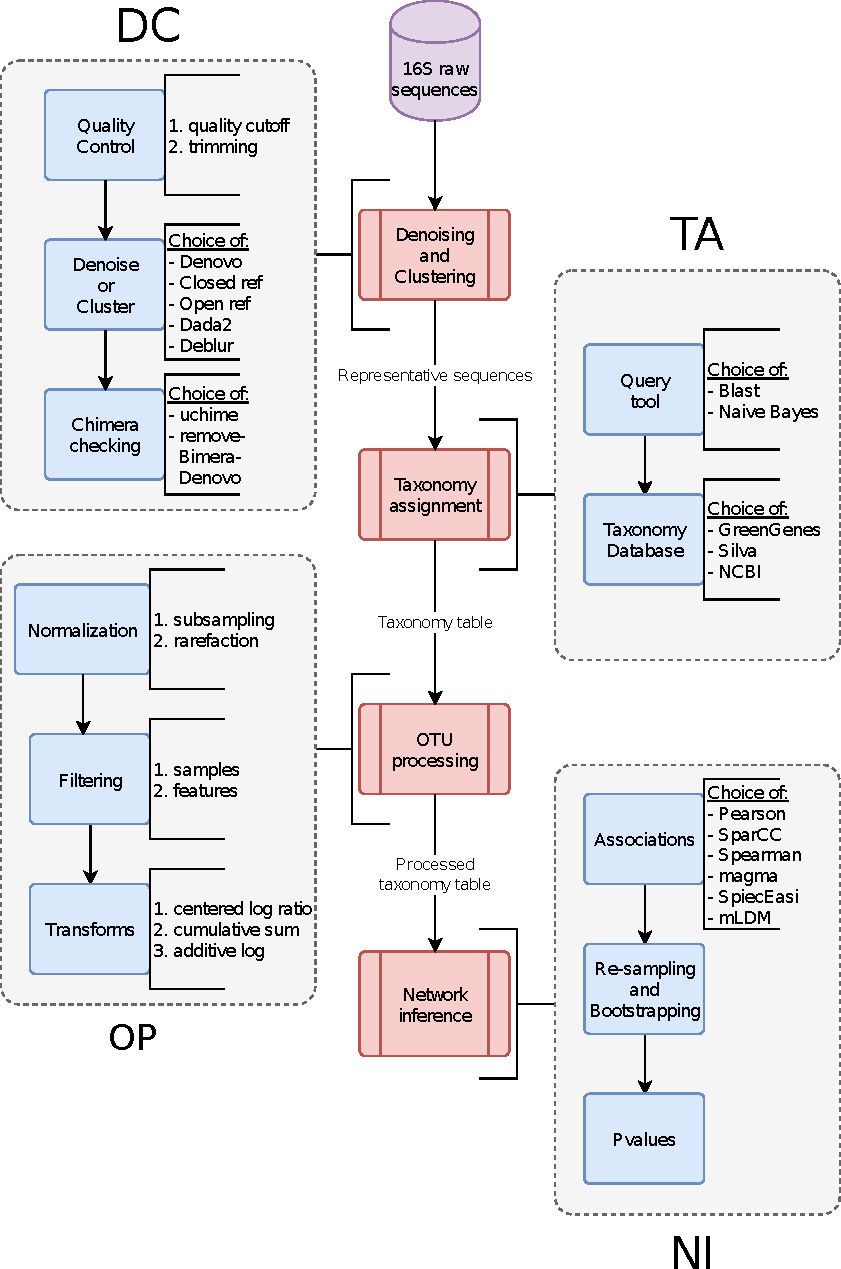
\includegraphics[width=0.74\linewidth]{figure1.pdf}
  % \end{figure}
  \begin{figure}[H]
    \centering
    \caption{
      \textbf{The workflow of the \ac{micone} pipeline}.
      The steps of the workflow can be broken down into five major groups: \textbf{(SP)} \textbf{S}equence \textbf{P}rocessing, \textbf{(DC)} \textbf{D}enoising and \textbf{C}lustering, \textbf{(TA)} \textbf{T}axonomy \textbf{A}ssignment, \textbf{(OP)} \textbf{O}TU and ESV \textbf{P}rocessing, and \textbf{(NI)} \textbf{N}etwork \textbf{I}nference.
      Each step incorporates several processes (blue boxes), each of which in turn has several alternative algorithms for the same task (indicated by the text to the right of the blue boxes).
      Each arrow describes the data that is being passed from one step to another.
      The inputs to the pipeline are 16S rRNA sequencing reads, and the final output is the consensus network generated from the inferred co-occurrence networks.
      For details on each process and the different outputs, see Methods.
    }
    \label{fig:figure1}
  \end{figure}



  % \FloatBarrier
  % \newpage
  % \begin{figure}[H]
  %   \centering
  %   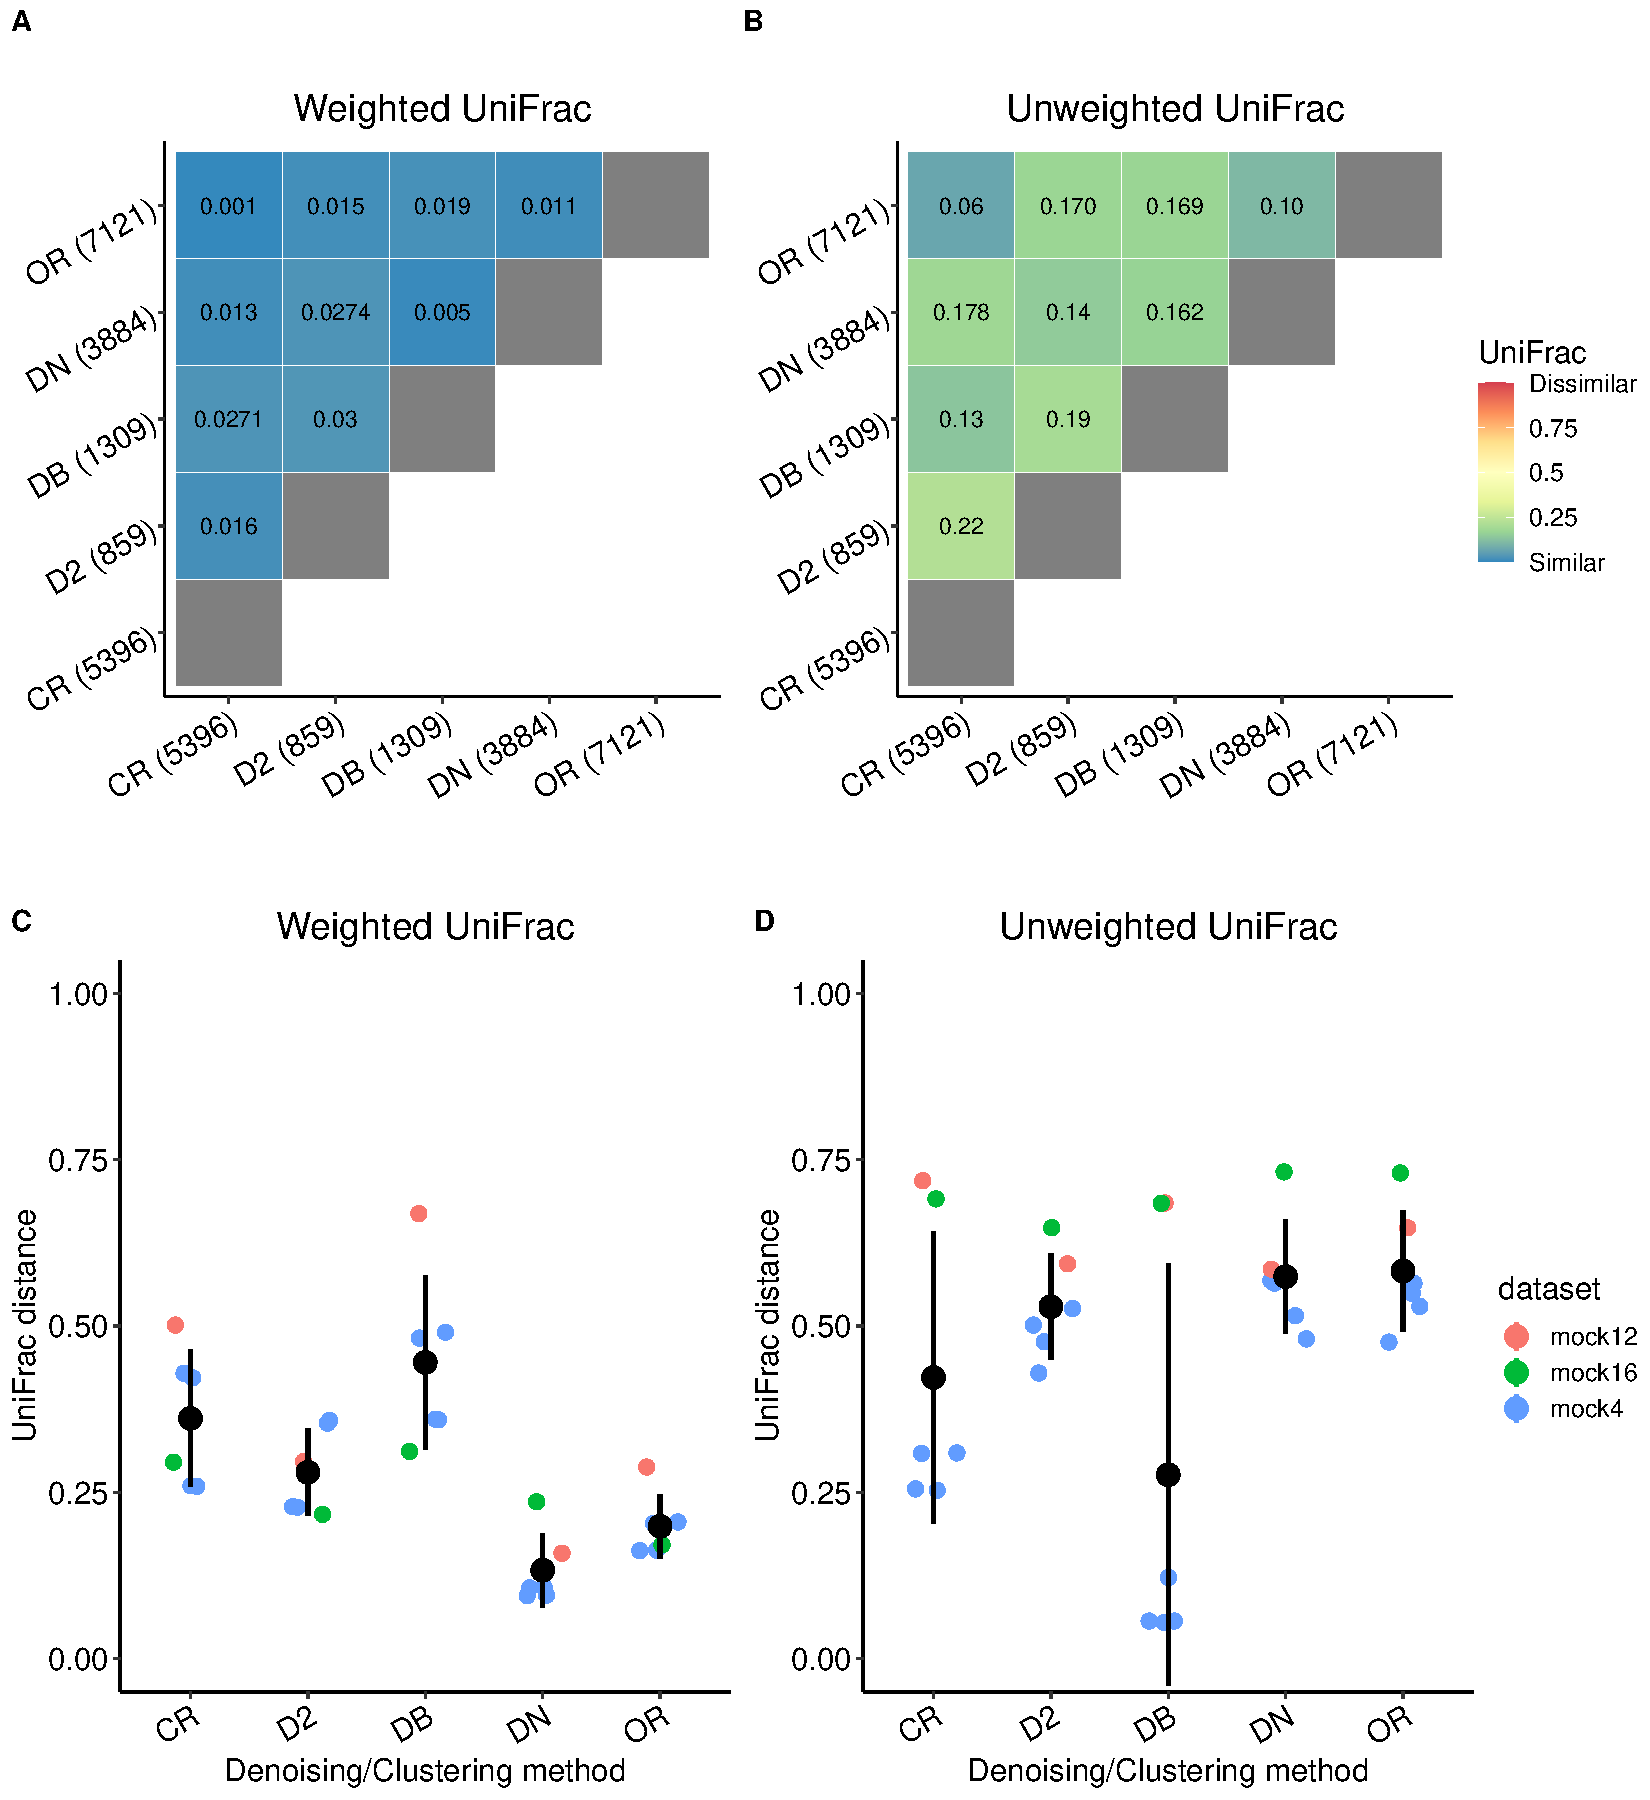
\includegraphics[width=\textwidth]{figure2.pdf}
  % \end{figure}
  \begin{figure}[H]
    \centering
    \caption{
      \textbf{The representative sequences generated by the different denoising and clustering methods differ in their identification of sequences that are low in abundance}.
      \textbf{(A)} The average weighted UniFrac distance between the representative sequences shows that the representative sequences and their compositions are fairly identical between the methods (with the exception of Deblur (DB) due to the low ESV count).
      \textbf{(B)} The relatively larger average unweighted UniFrac distance indicates that methods differ in their identification of sequences that are lower in abundance.
      The number of \ac{otu}s or \ac{esv}s generated by the respective methods are provided in the parenthesis next to their names.
      The data used for the analysis in (A, B) were the samples from the fecal microbiome transplant (FMT) dataset~\cite{Kang2017}, containing both healthy subjects and subjects with autism spectrum disorder (ASD).
      \textbf{(C, D)} The distributions of the average weighted and unweighted UniFrac distance between the predicted sequence profile and the expected sequence profile in the mock datasets.
      The average weighted UniFrac distances show that de novo (DN) and open reference (OR) were the best-performing methods in most of the datasets, while they are the worst-performing methods under the unweighted UniFrac metric.
      The good performance of dada2 (D2) under both distance metrics combined with its approach of identifying \ac{esv}s using de novo methods, prompts us to use it as the default method for the DC step.
      The data used for the analysis in (C, D) were the mock4, mock12, and mock16 datasets from mockrobiota~\cite{Bokulich2016}.
    }
    \label{fig:figure2}
  \end{figure}


  % \FloatBarrier
  % \newpage
  % \begin{figure}[H]
  %   \centering
  %   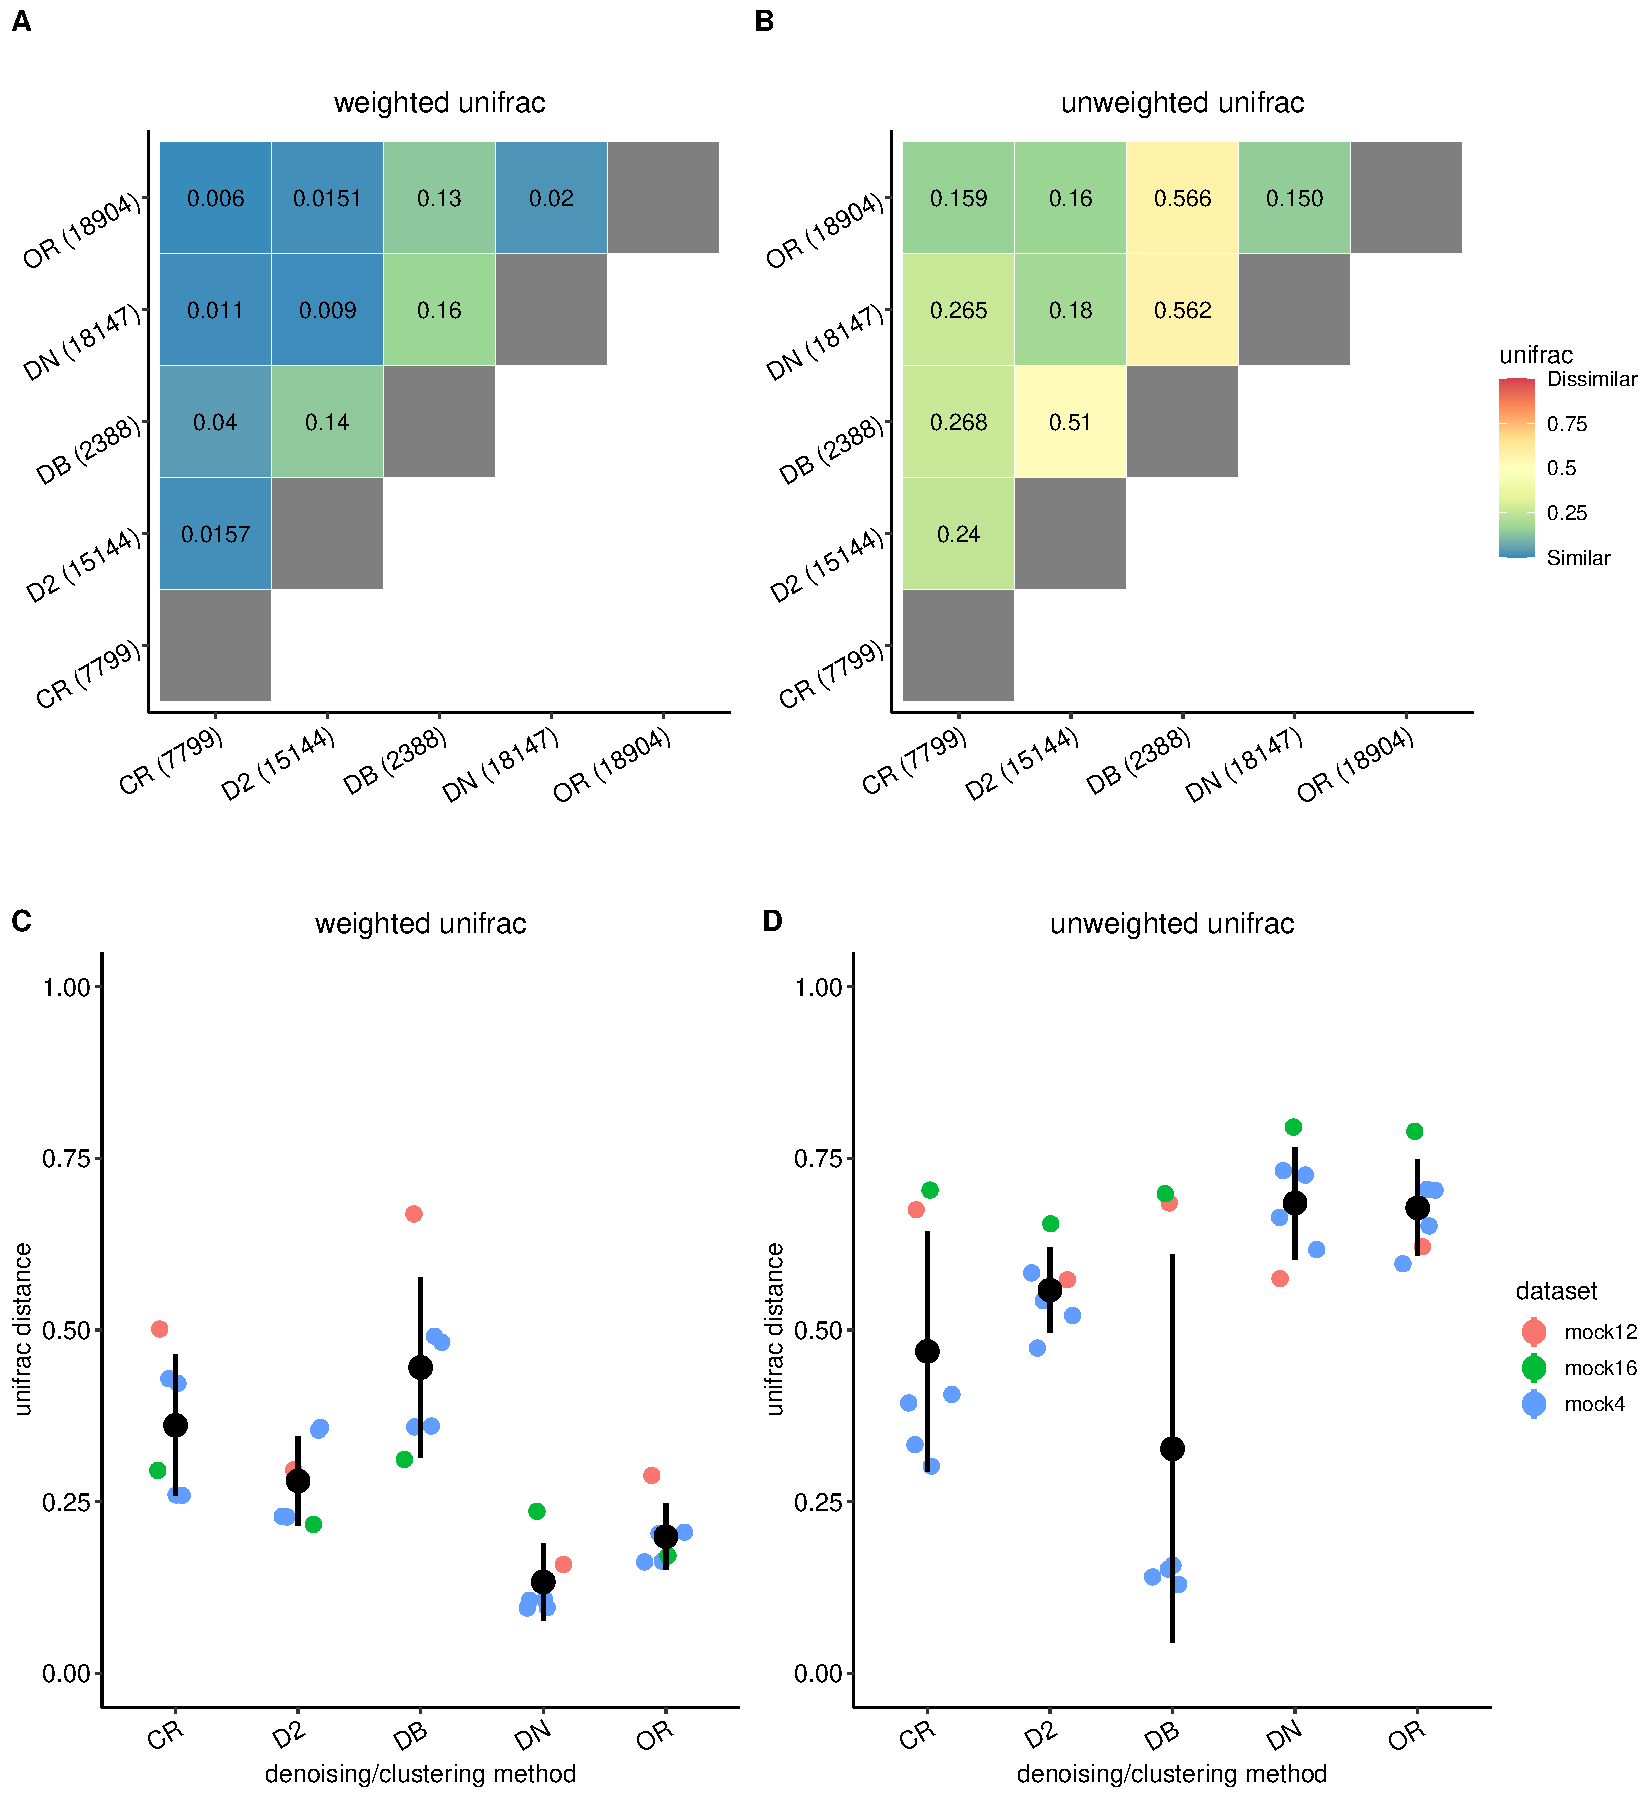
\includegraphics[width=\textwidth]{figure3.pdf}
  % \end{figure}
  \begin{figure}[H]
    \centering
    \caption{
      \textbf{Taxonomic reference databases vary in terms of their taxonomy assignments below the Order level}.
      \textbf{(A)} The taxonomic assignments of the top 50 representative sequences using the three different reference databases.
      This result illustrates how the same sequences are assigned to different genera under different databases.
      A significant portion of the representative sequences are assigned to an ``unknown'' Genus in two of three databases (\ac{gg} and \ac{ncbi}).
      The number of assigned genera for each database is displayed at the top of each column.
      \textbf{(B)} The number of representative sequences assigned to the same taxonomic label when using different reference databases (for the top 100 sequences).
      The mismatches are fewer at higher taxonomic levels, but, even at the Order level there exists greater than 51\% of mismatches, demonstrating the poor agreement in taxonomic labels assigned by the different databases.
      The data used for the analysis in (A, B) were samples (healthy and ASD) from the FMT dataset.
      \textbf{(C)} The Bray-Curtis dissimilarity between the predicted taxonomy profile and expected taxonomy profile in the mock datasets shows that there is no singular best choice of database for every dataset, as all the databases show similar performances.
      The \ac{gg} database and the Naive Bayes classifier are chosen as the defaults for the TA step of \ac{micone} due to their popularity.
      The datasets used for the analysis in (C) were the mock datasets from mockrobiota.
    }
    \label{fig:figure3}
  \end{figure}


  % \FloatBarrier
  % \newpage
  % \begin{figure}[H]
  %   \centering
  %   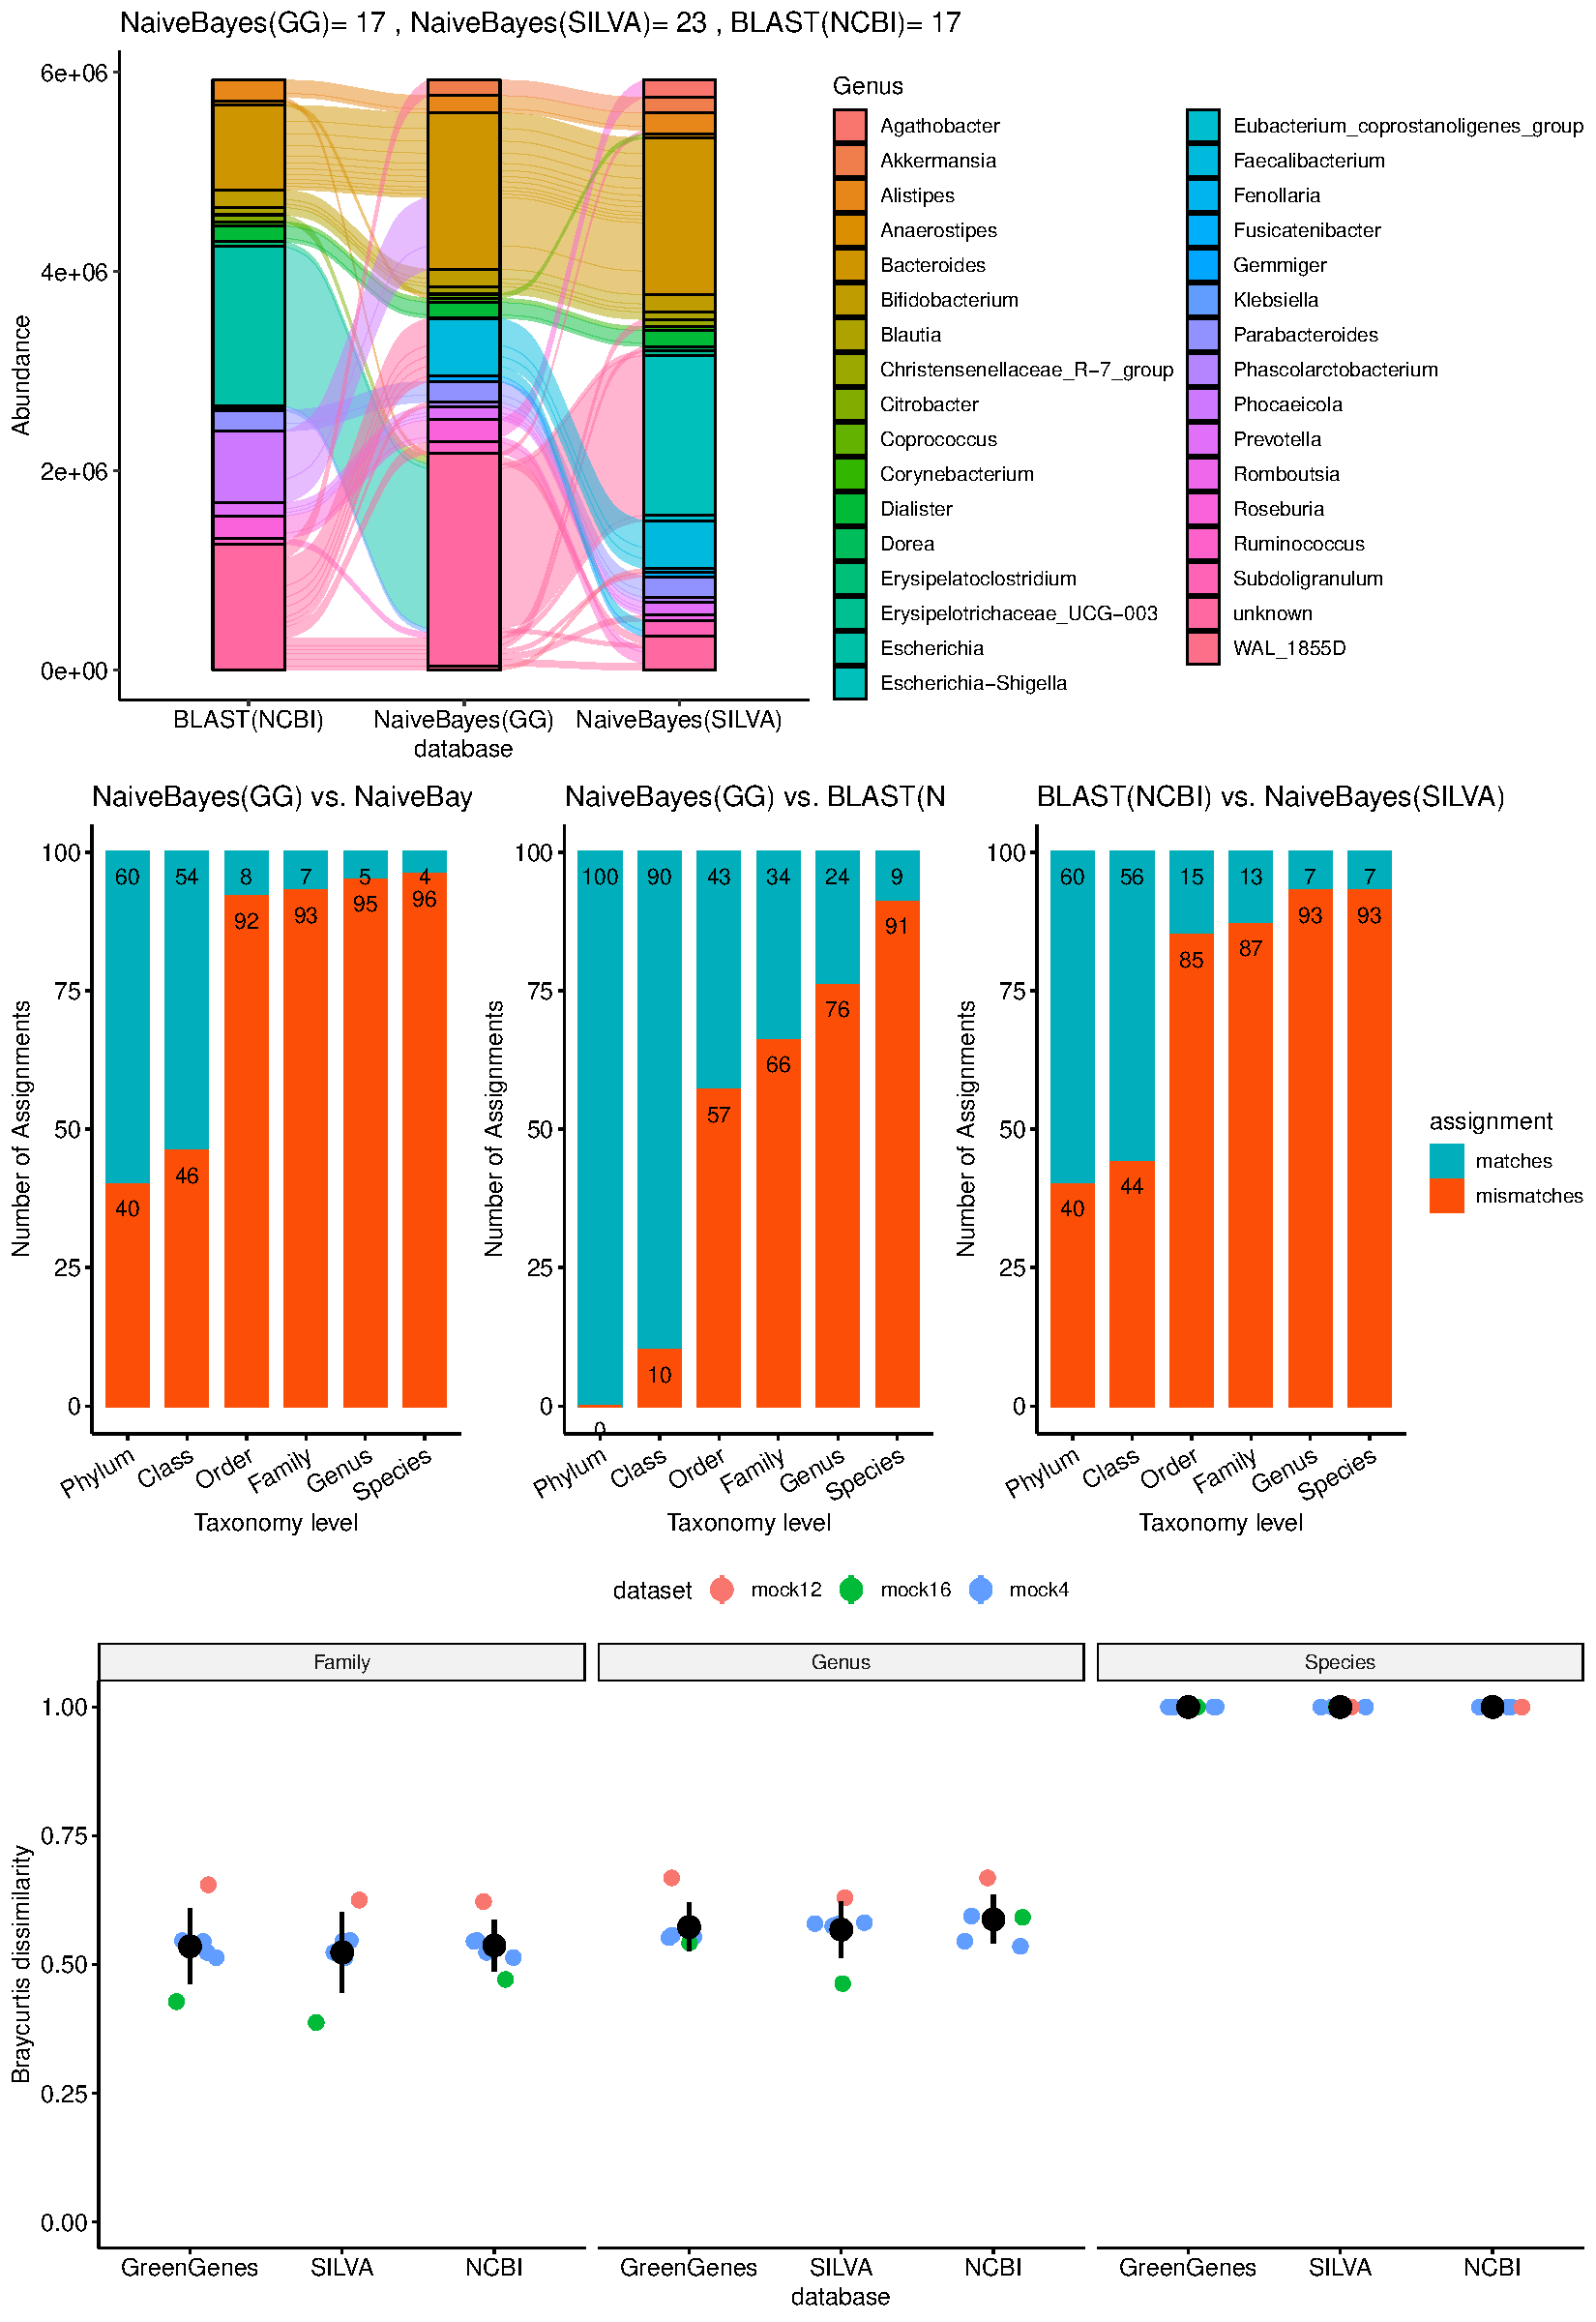
\includegraphics[width=\textwidth]{figure4.pdf}
  % \end{figure}
  \begin{figure}[H]
    \centering
    \caption{
      \textbf{Networks generated using different network inference methods show notable differences in terms of edge-density and connectivity}.
      \textbf{(A)} The nine different networks (excluding \acs{mldm}) generated by the different network inference methods.
      The nodes for each network (representing taxa) are arranged in the same positions in a circular layout and the differences in the connections can be directly visualized and compared.
      The green links are positive associations and the orange links represent negative associations.
      The networks look dissimilar and vary widely in terms of connectivity, and it is notable that the correlation-based methods generally produce networks with higher edge-densities.
      A threshold of 0.3 was set for the correlation-based methods (sparcc, propr, spearman and pearson) and a threshold of 0.01 was set for the direct association methods (flashweave, spieceasi, cozine, harmonies, and spring).
      \textbf{(B)} The node overlap Upset plot indicates that all the networks have a large proportion of common nodes involved in connections (33 out of 68).
      Conversely \textbf{(C)}, the edge overlap Upset plot shows that a very small fraction of these connections are actually shared (8 out of 202).
      The data used in this analysis were the healthy stool samples from the FMT dataset.
      \acs{mldm} is not shown in the comparisons because the algorithm failed to converge for the particular network combination used here (default setting of the \ac{micone} pipeline).
    }
    \label{fig:figure4}
  \end{figure}


  % \FloatBarrier
  % \newpage
  % \begin{figure}[H]
  %   \centering
  %   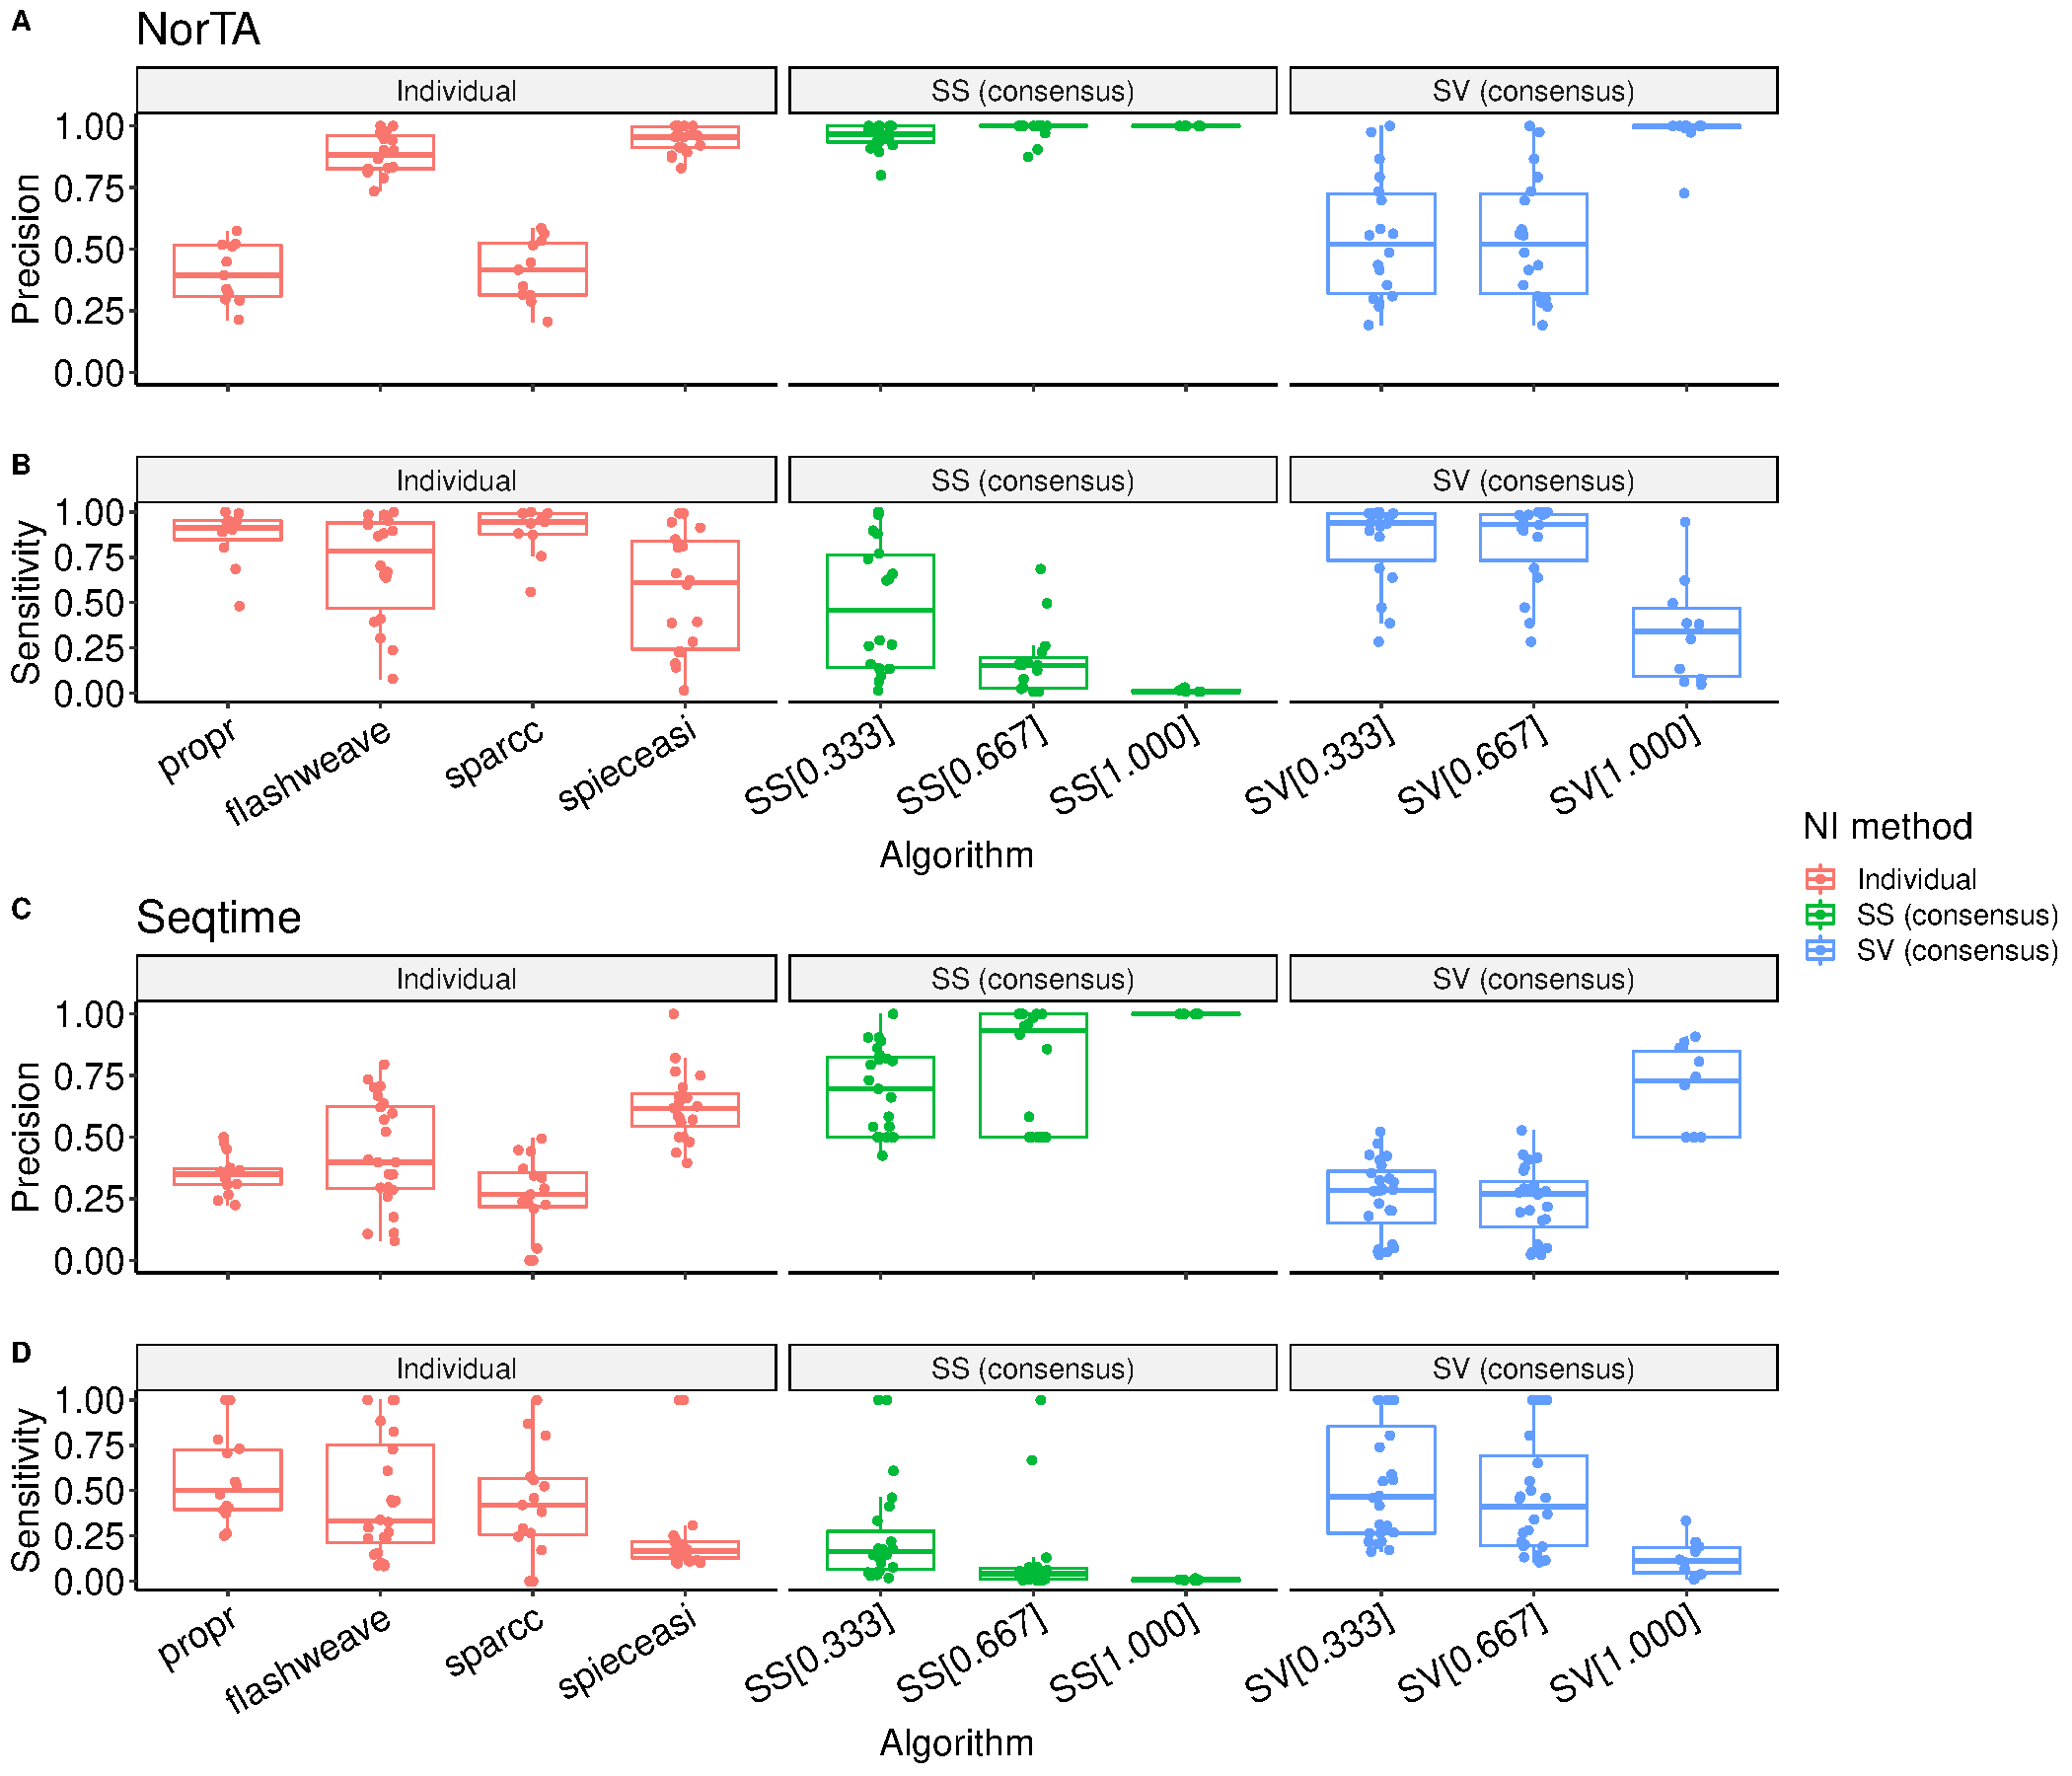
\includegraphics[width=1.0\linewidth]{figure5.pdf}
  % \end{figure}
  \begin{figure}[H]
    \centering
    \caption{
      \textbf{The associations generated by the scaled-sum consensus method show high precision in benchmarks using synthetic datasets}.
    The different points on the box plot show the precision (red) and sensitivity (blue) of co-occurrence networks generated through individual network inference methods and through consensus network construction approaches. Precision and sensitivity are estimated based on the comparisons with two sets of synthetic benchmark datasets (``NorTA'' and ``seqtime'', see Methods).
      The independent algorithms chosen for the comparison are the two best-performing correlation-based (propr, sparcc) and direct association based (spieceasi, flashweave) methods.
      For consensus network inference, we used the scaled-sum (SS) and simple voting (SV) methods.
      A weight threshold of 0.1 and a p-value threshold of 0.05 was applied to each network before the calculation of precision and sensitivity.
      The purpose behind the construction of the consensus algorithms is to capture true associations in the data through the removal of assocations that have a lower probability of being present in the networks inferred by different inference algorithms.
      Therefore, an increase in precision is followed by a decrease in sensitivity.
      The overall best precision was consistently obtained by the scaled-sum consensus method for $\theta \geq 0.333$ on both benchmark datasets. Among all the individual network inference methods, spieceasi shows the best average precision.
      The simple voting method, when using the presence of edges in all inferred networks as a requirement ($\theta = 1.000$), also outperforms spieceasi on average precision.
      Therefore, we set the scaled-sum consensus method with $\theta = 0.333$ as the default tool for consensus network inference, since this option provides a good balance of precision and sensitivity (see also Figure~\ref{fig:figure_s5} and \ref{fig:figure_s6}).
      The correlation-based methods (propr, and \acs{sparcc}) and the simple-voting consensus method return networks with higher sensitivities.
    }
    \label{fig:figure5}
  \end{figure}


  % \FloatBarrier
  % \newpage
  % \begin{figure}[H]
  %   \centering
  %   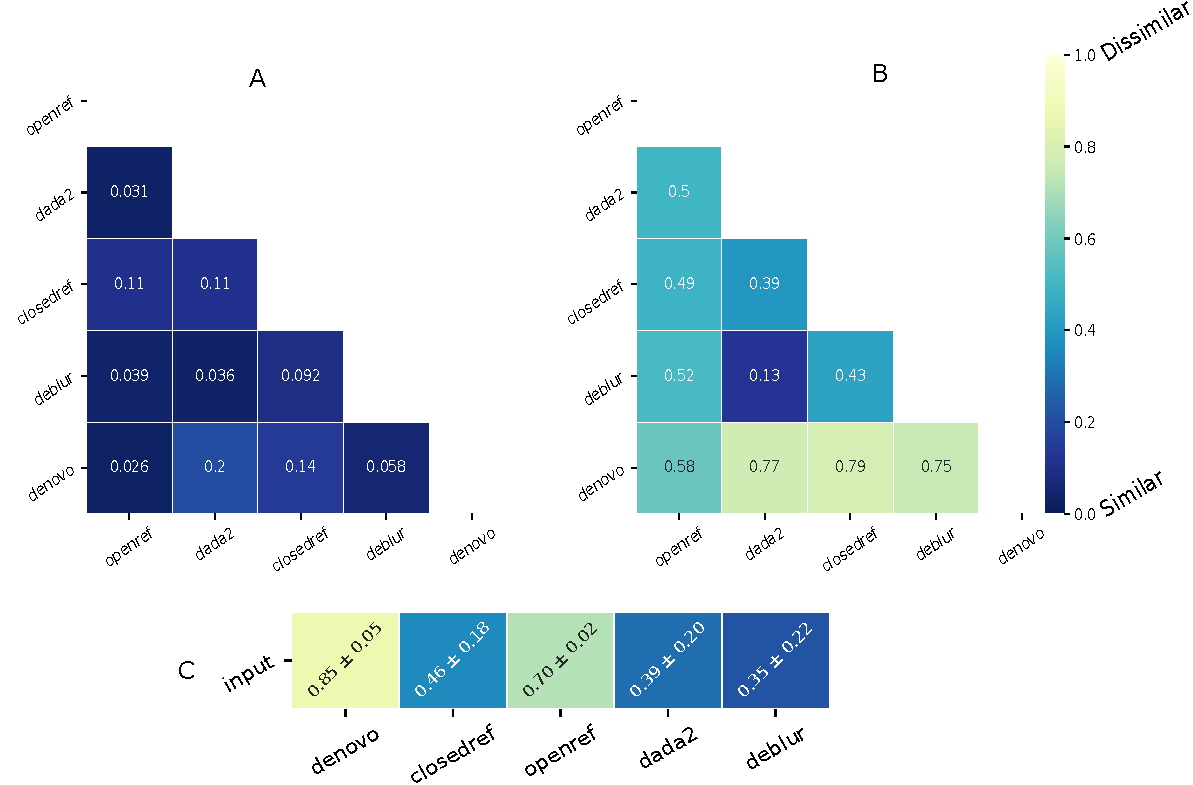
\includegraphics[width=\textwidth]{figure6.pdf}
  % \end{figure}
  \begin{figure}[H]
    \centering
      \caption{
      \textbf{The choice of reference database has the largest impact on network variance}.
      \textbf{(A)} The percentage of variance in the networks (from the  FMT dataset) contributed by the \acf{dc}, CC (chimera checking), \acf{ta}, \acf{op} and \acf{ni} steps of the pipeline calculated using ANOVA on a linear model (see Methods).
      A weight threshold of 0.1 and a p-value threshold of 0.05 were applied to each network before the analysis.
      The taxonomy database contributes most to the variance between the networks (65.4\%) followed by the filtering of the counts matrix (26.8\%) in the OP step.
    The variation due to the NI, DC and CC steps are much smaller in comparison (6.553\%, 0.648\%, and 0.003\% respectively).
      The negligible fraction labeled as the residual is an artifact that arises when multiple steps are changed at the same time.
      \textbf{(B)} All the inferred networks generated from various combinations of tools are shown as points on a PCA plot.
      Each point on the PCA plot represents a network inferred using different combinations of tools and parameters that are available in the \ac{micone} pipeline.
      The color of the points corresponds to the tools used at each step of the pipeline (DC, TA, OP, and NI).
      The points on the PCA plot can be grouped based on the TA step, but the extent of this separation decreases when the filtering is turned on in the OP step, confirming that the variability in the networks decreased upon filtering out the taxonomic entities at low abundance.
      Some algorithms, especially the direct association methods, at the NI step can also be seen to generate networks that are less variable compared to the others.
      The \ac{dc} step does not seem to have any correlation with the variation in the networks on the PCA plot.
    }
    \label{fig:figure6}
  \end{figure}


  % \FloatBarrier
  % \newpage
  % \begin{figure}[H]
  %   \centering
  %   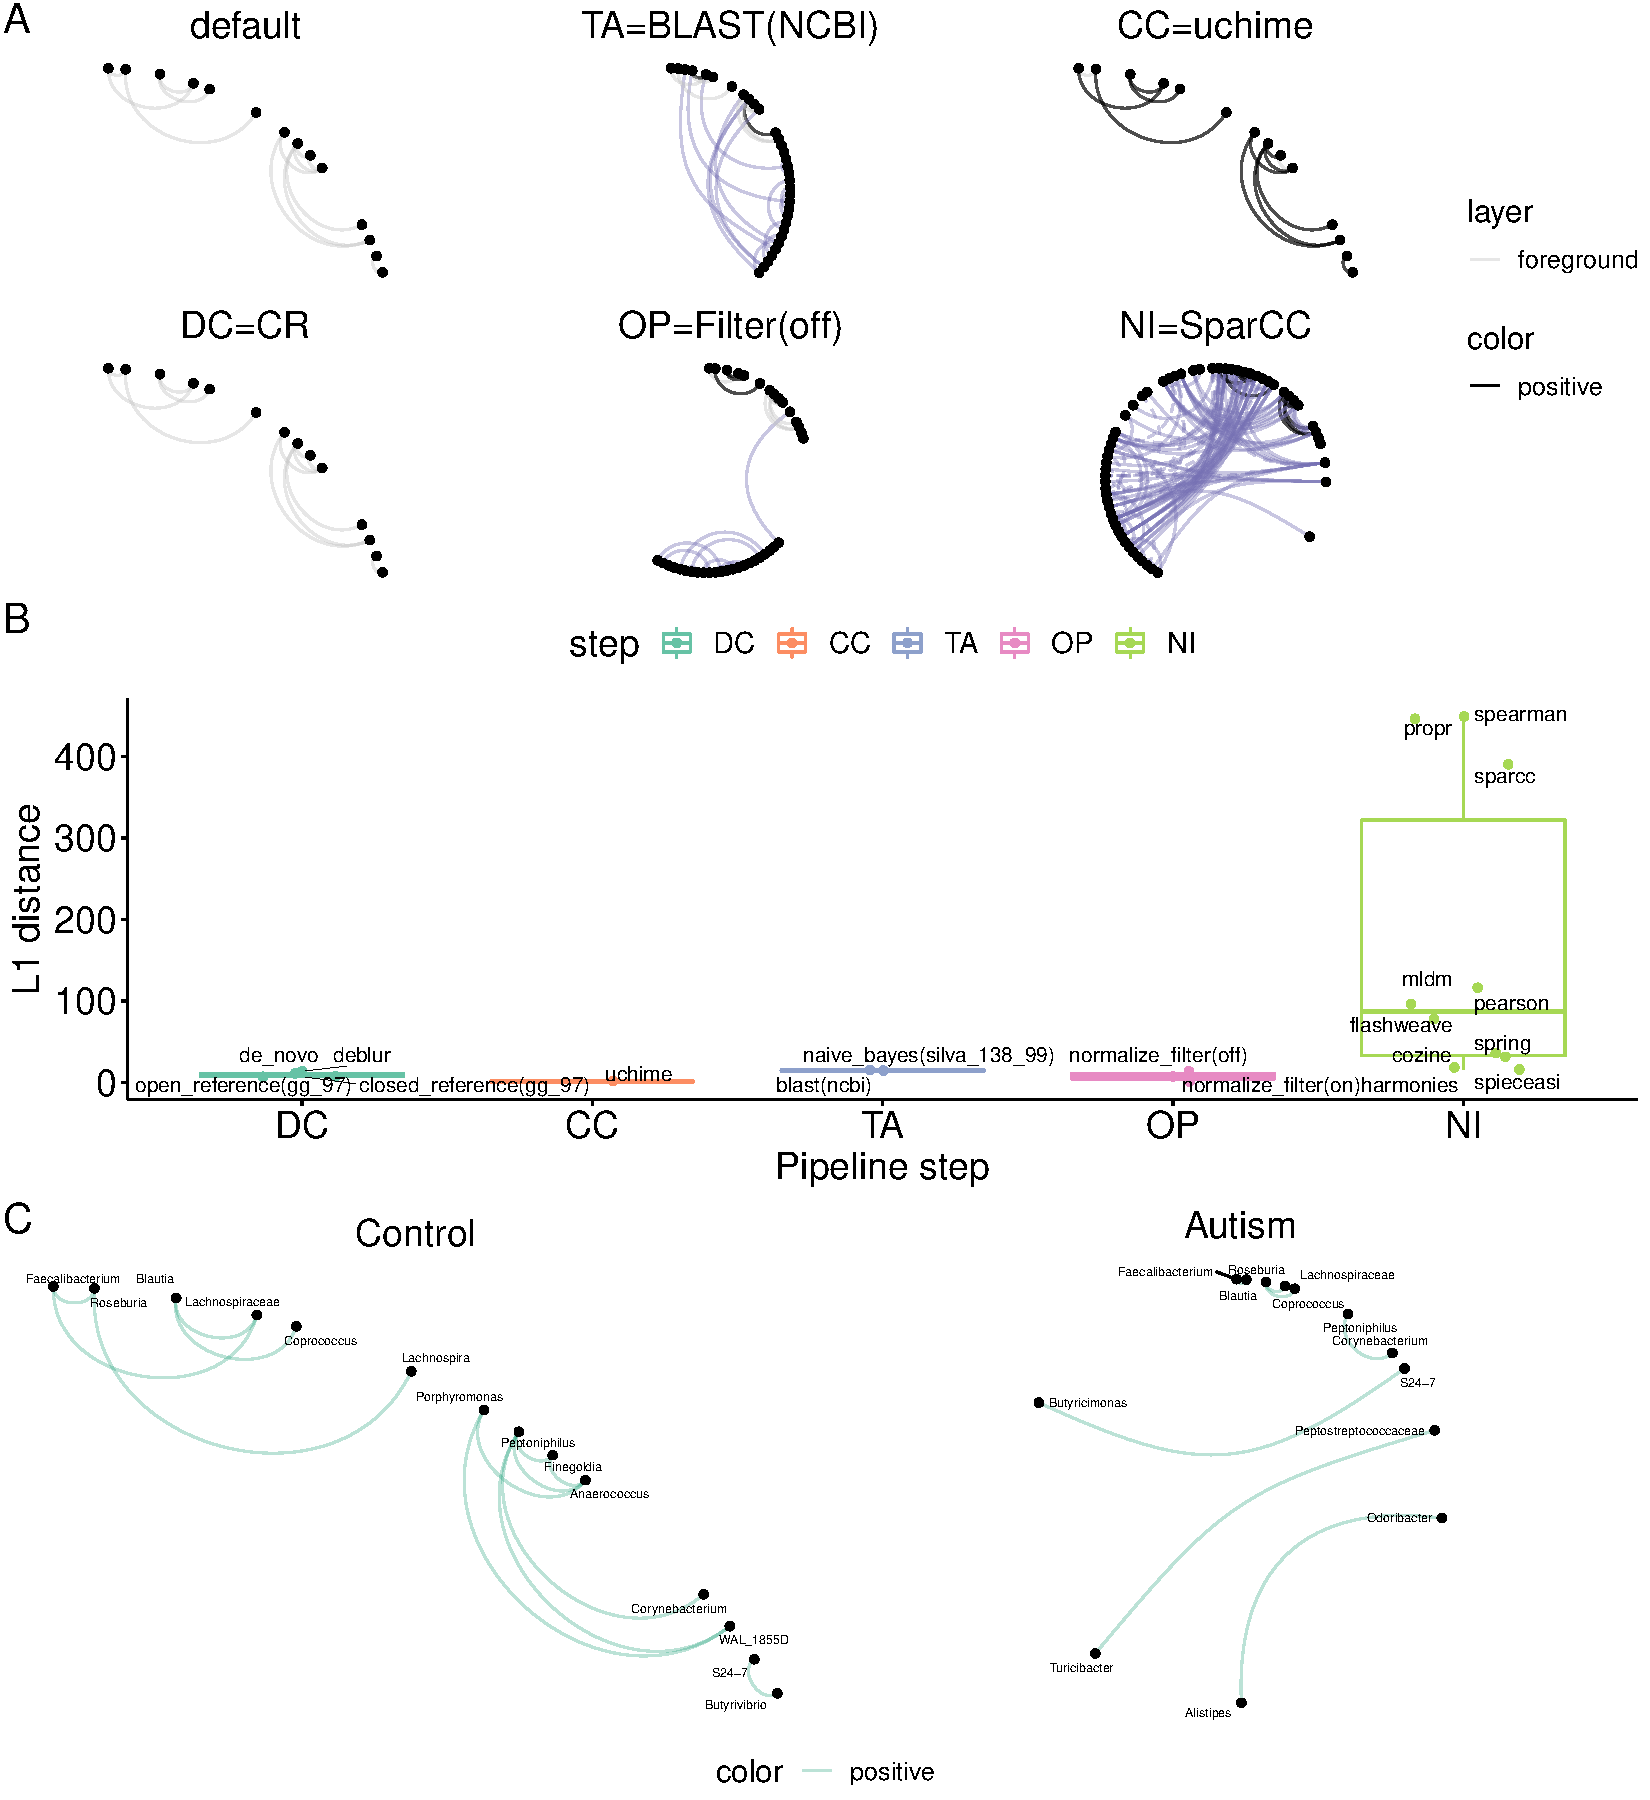
\includegraphics[width=1.0\linewidth]{figure7.pdf}
  % \end{figure}
  \begin{figure}[H]
    \centering
    \caption{
      \textbf{Comparison of networks generated from the control and ASD samples of the FMT dataset using the \ac{micone} pipeline}.
      The networks for the control (left) and ASD (right) samples were generated using the default tools and parameters recommended by the \ac{micone} pipeline as described in Table~\ref{tab:micone_tools}.
      There are 22 unique links in the network for control samples, 12 unique links in the network for ASD subjects, and 7 edges in common between both networks.
      The changes in these connections can serve as potential starting points for further experimental validations or literature surveys.
    }
    \label{fig:figure7}
  \end{figure}


  \FloatBarrier
  \newpage
  \subsection*{Supplementary Tables and Figures}

  \renewcommand{\thefigure}{S\arabic{figure}}
  \setcounter{figure}{0}

  \renewcommand{\thetable}{S\arabic{table}}
  \setcounter{table}{0}

  \begin{table}[H]
    \centering
    \caption{
      \textbf{Table of global network metrics for networks inferred from all possible combinations of tools}.
      In each row, one tool in a particular step is kept constant, and the metric is calculated for every possible combination of tools for the other steps of the pipeline.
      Therefore, each row shows the grouped average metric for each tool in every step of the pipeline.
      The network inference methods show the most variation in the global network metrics compared to tools in other steps of the pipeline.
    }
    \label{tab:network_metrics}
  \end{table}


    % \begin{figure}[H]
    %   \centering
    %   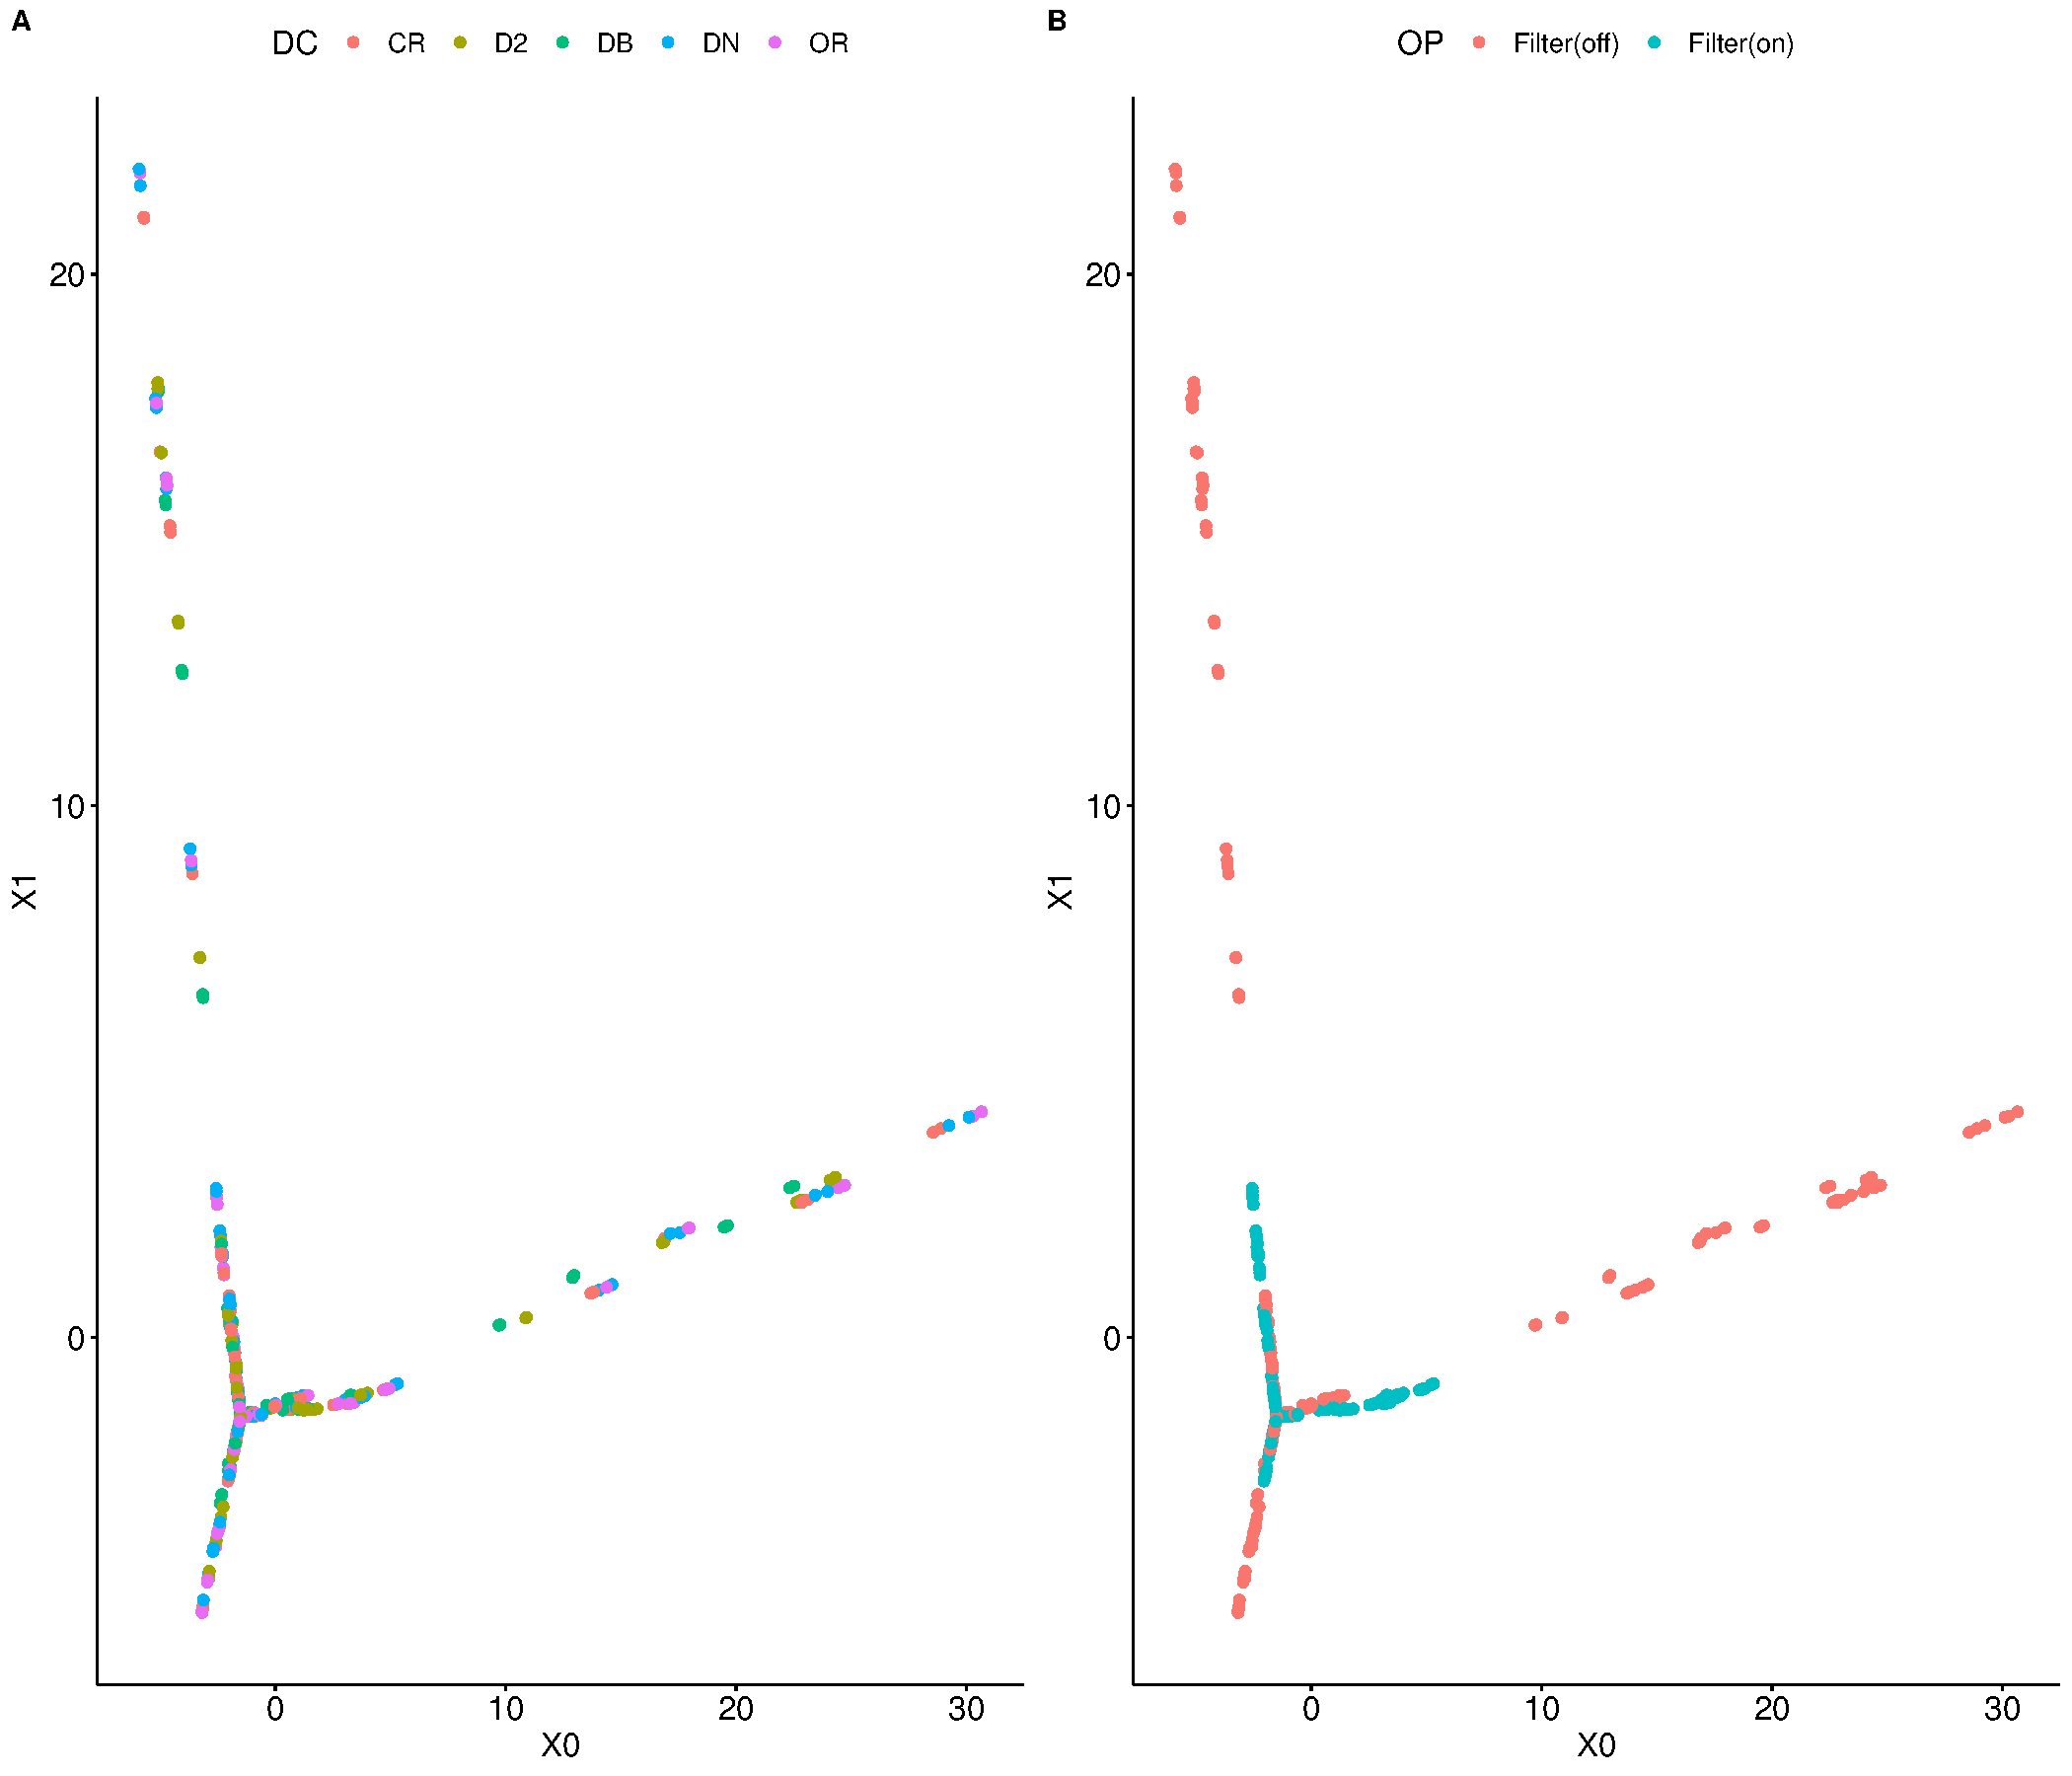
\includegraphics[width=1.0\linewidth]{figure_s1.pdf}
    % \end{figure}
    \begin{figure}[H]
      \centering
        \caption{
          \textbf{The t-SNE plot of all the inferred networks clusters the networks based on the taxonomy reference database used}.
          Each point on the t-SNE plot represents a network inferred using different combinations of tools and parameters that are available in the \ac{micone} pipeline.
          The points are colored by the tools and parameters used in \ac{dc} step (A), \ac{ta} step (B), \ac{op} step (C) and \ac{ni} step (D).
          The separation of the points based on taxonomy reference database shows that the points cluster based on reference database in high-dimensional space.
        }
      \label{fig:figure_s1}
    \end{figure}
    % \FloatBarrier
    % \newpage

    % \begin{figure}[H]
    %   \centering
    %   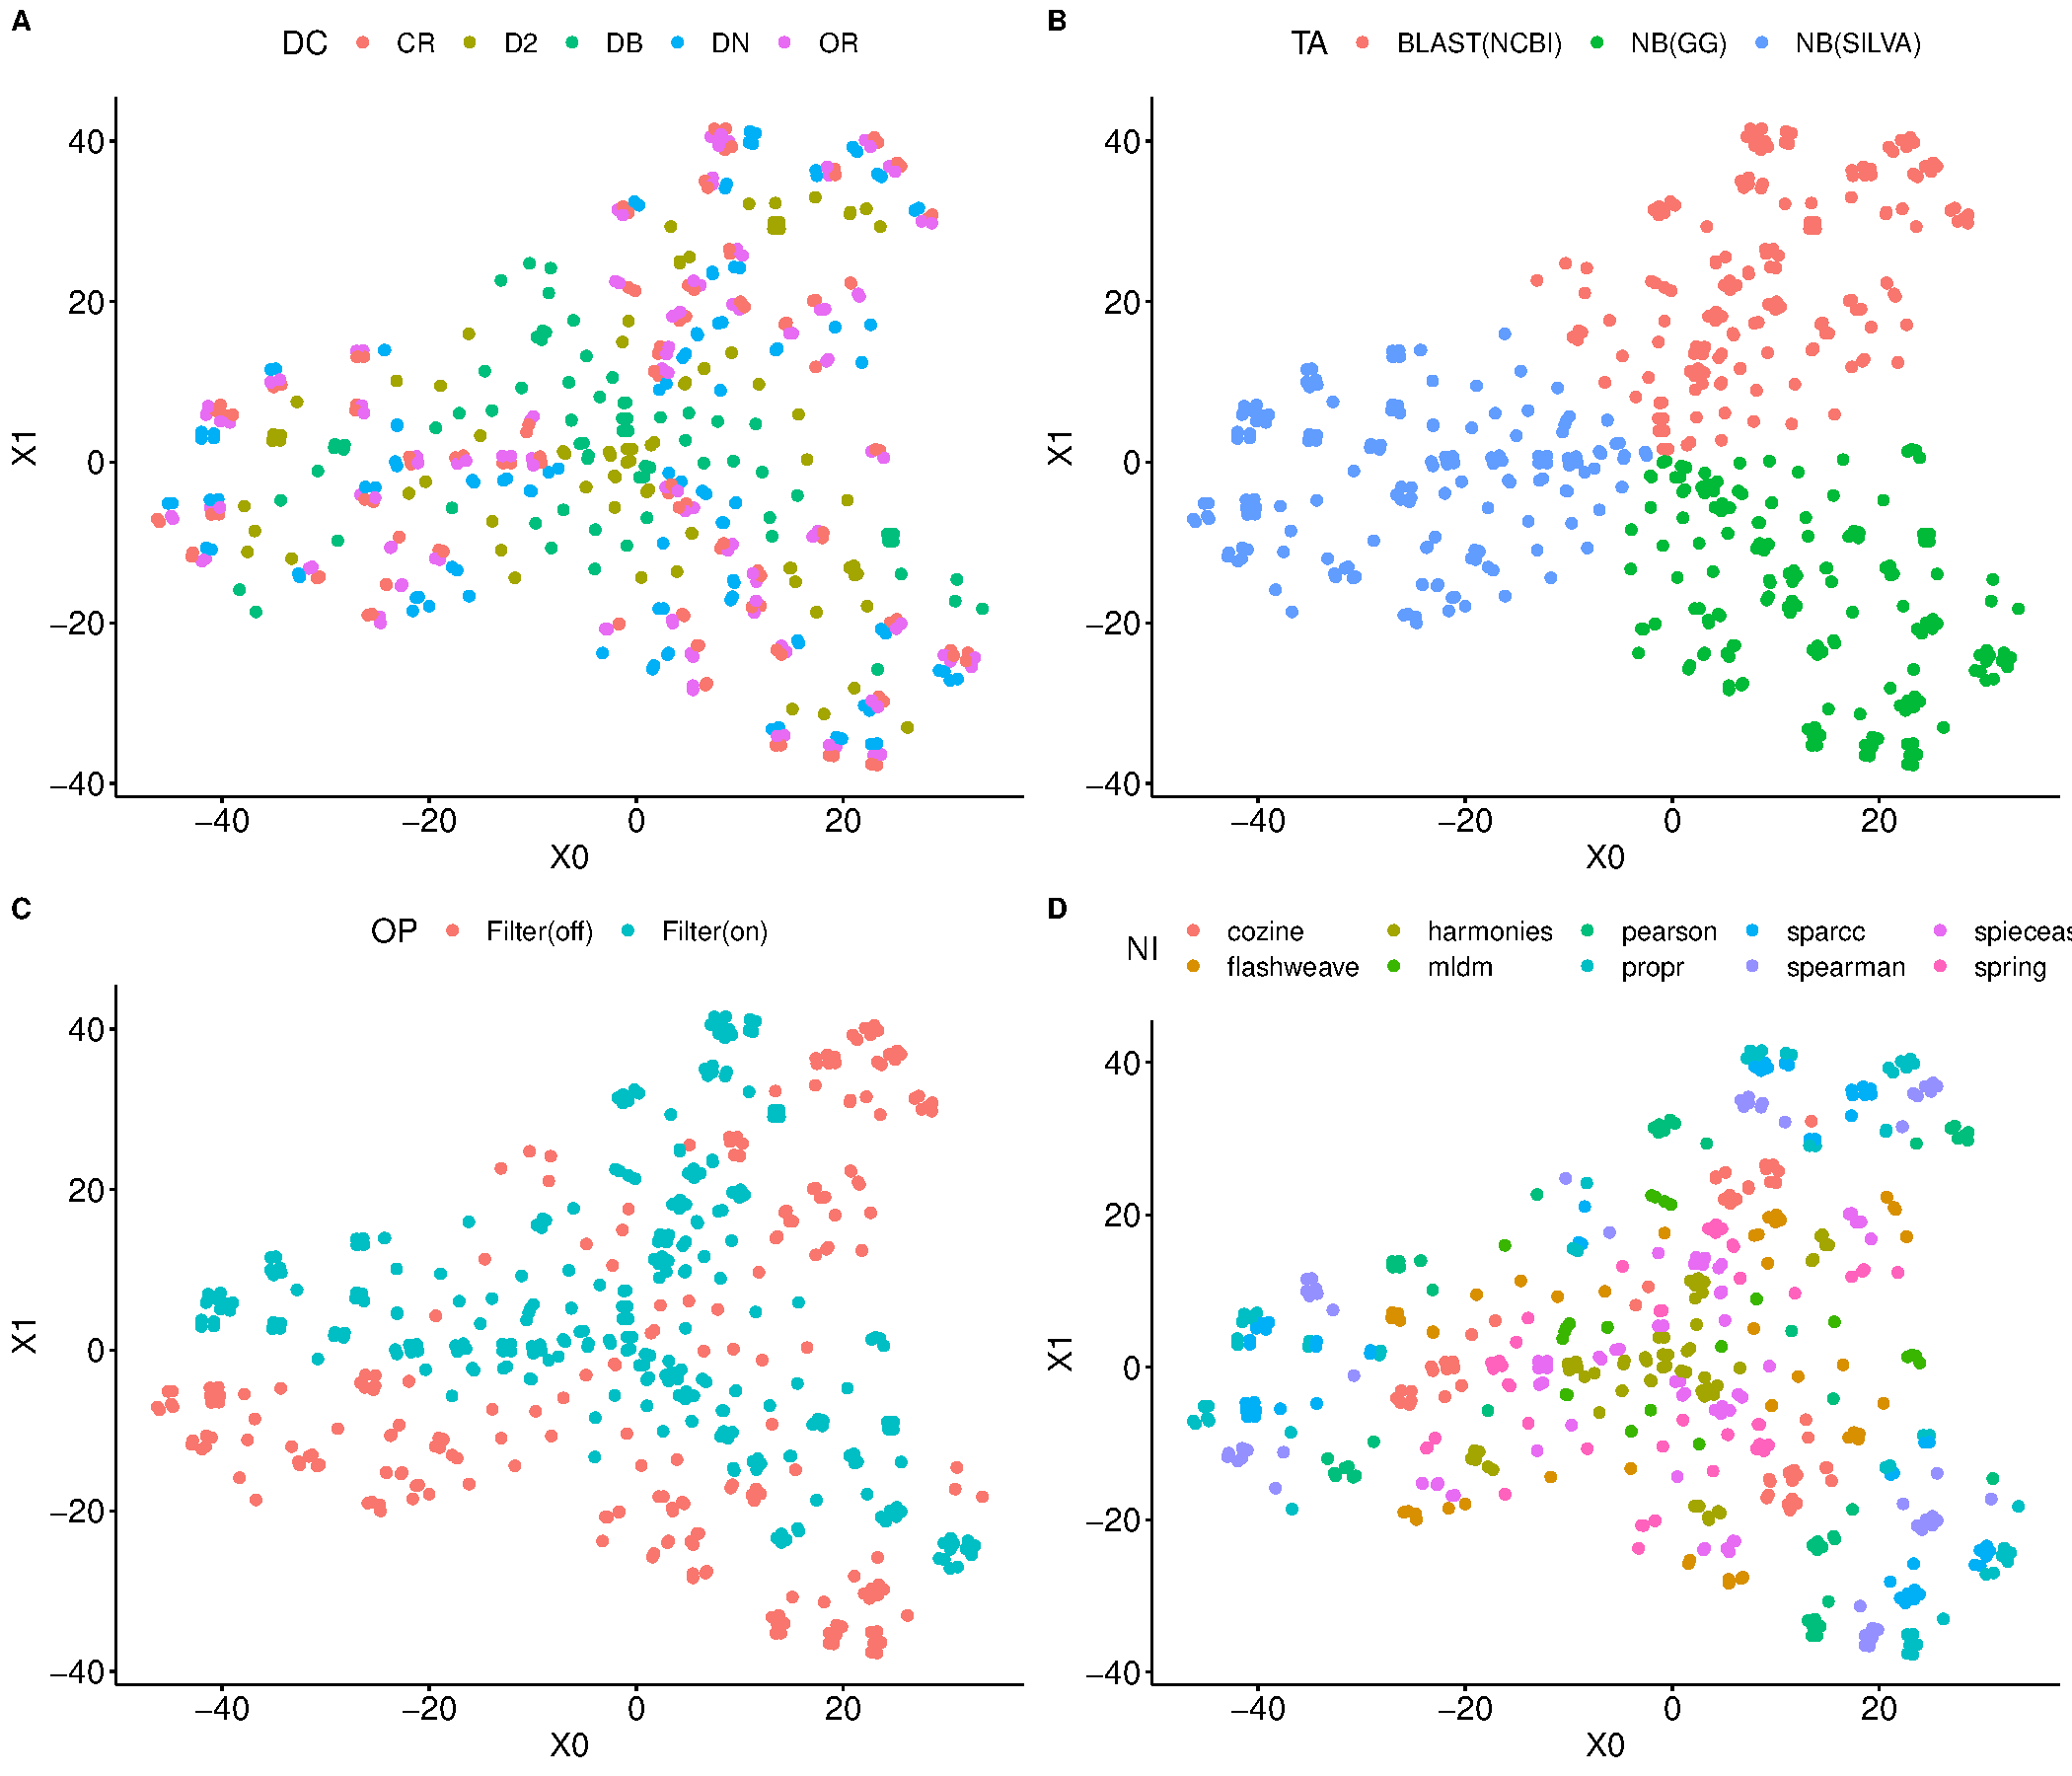
\includegraphics[width=1.0\linewidth]{figure_s2.pdf}
    % \end{figure}
    \begin{figure}[H]
      \centering
        \caption{
          \textbf{The UniFrac distance between the 1000 most abundant representative sequences is higher than that when all sequences are considered}.
          Each value is the average UniFrac distance between the reference sequences generated by the various methods in the \ac{dc} step (similar to Figure~\ref{fig:figure2}).
          There is an increase in both weighted and unweighted UniFrac distances compared to when all the representative sequences are considered.
          This shows that the 1000 most abundant representative sequences generated by the DC methods are not as similar to each other.
          And since the weighted UniFrac is much smaller than the unweighted UniFrac distance, we can conclude that those reference sequences that are present in the middle of the abundance distribution (considering all sequences) are dissimilar.
        }
      \label{fig:figure_s2}
    \end{figure}
    % \FloatBarrier
    % \newpage

    % \begin{figure}[H]
    %   \centering
    %   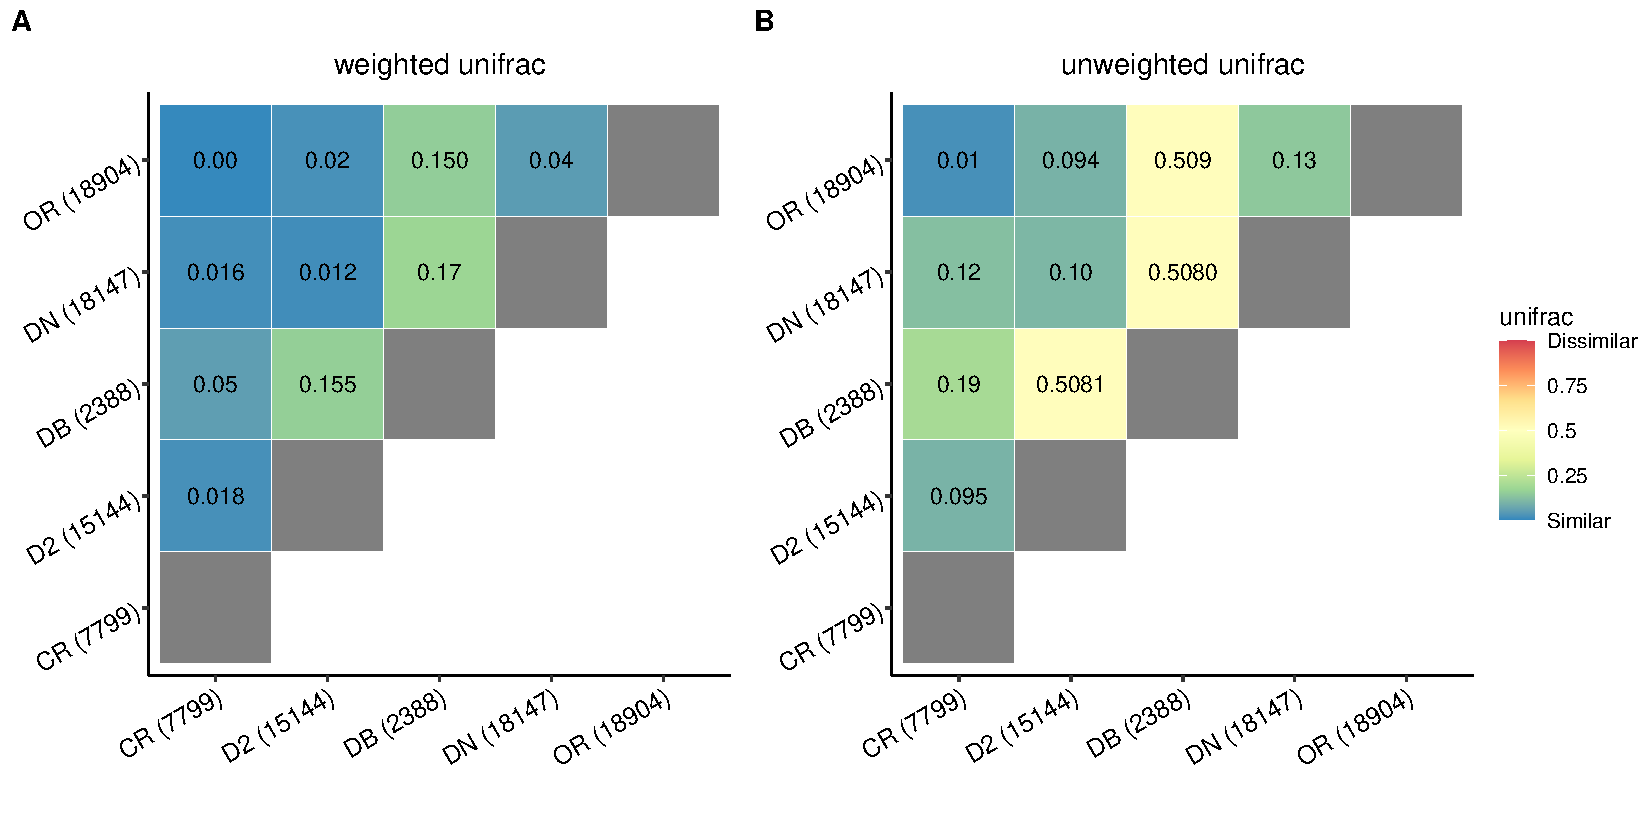
\includegraphics[width=1.0\linewidth]{figure_s3.pdf}
    % \end{figure}
    \begin{figure}[H]
      \centering
        \caption{
          \textbf{The weighted and unweighted UniFrac distances are small for the representative sequences generated using remove bimera and uchime for each denoising method}.
          With the exception of de novo and open reference under the unweighted UniFrac metric, all the other methods have high similarity, implying that the two chimera checking methods, uchime and remove bimera, produce similar outputs.
          This is especially true for the \ac{dada2} and Deblur methods which are the recommended denoising methods in the \ac{micone} pipeline.
          Therefore, remove bimera is recommended as the default chimera method if one is using \ac{dada2} and uchime-denovo when one is using Deblur, since these methods were developed for these respective algorithms (\ac{qiime2} uses uchime-denovo in the Deblur workflow).
        }
      \label{fig:figure_s3}
    \end{figure}
    % \FloatBarrier
    % \newpage

    % \begin{figure}[H]
    %   \centering
    %   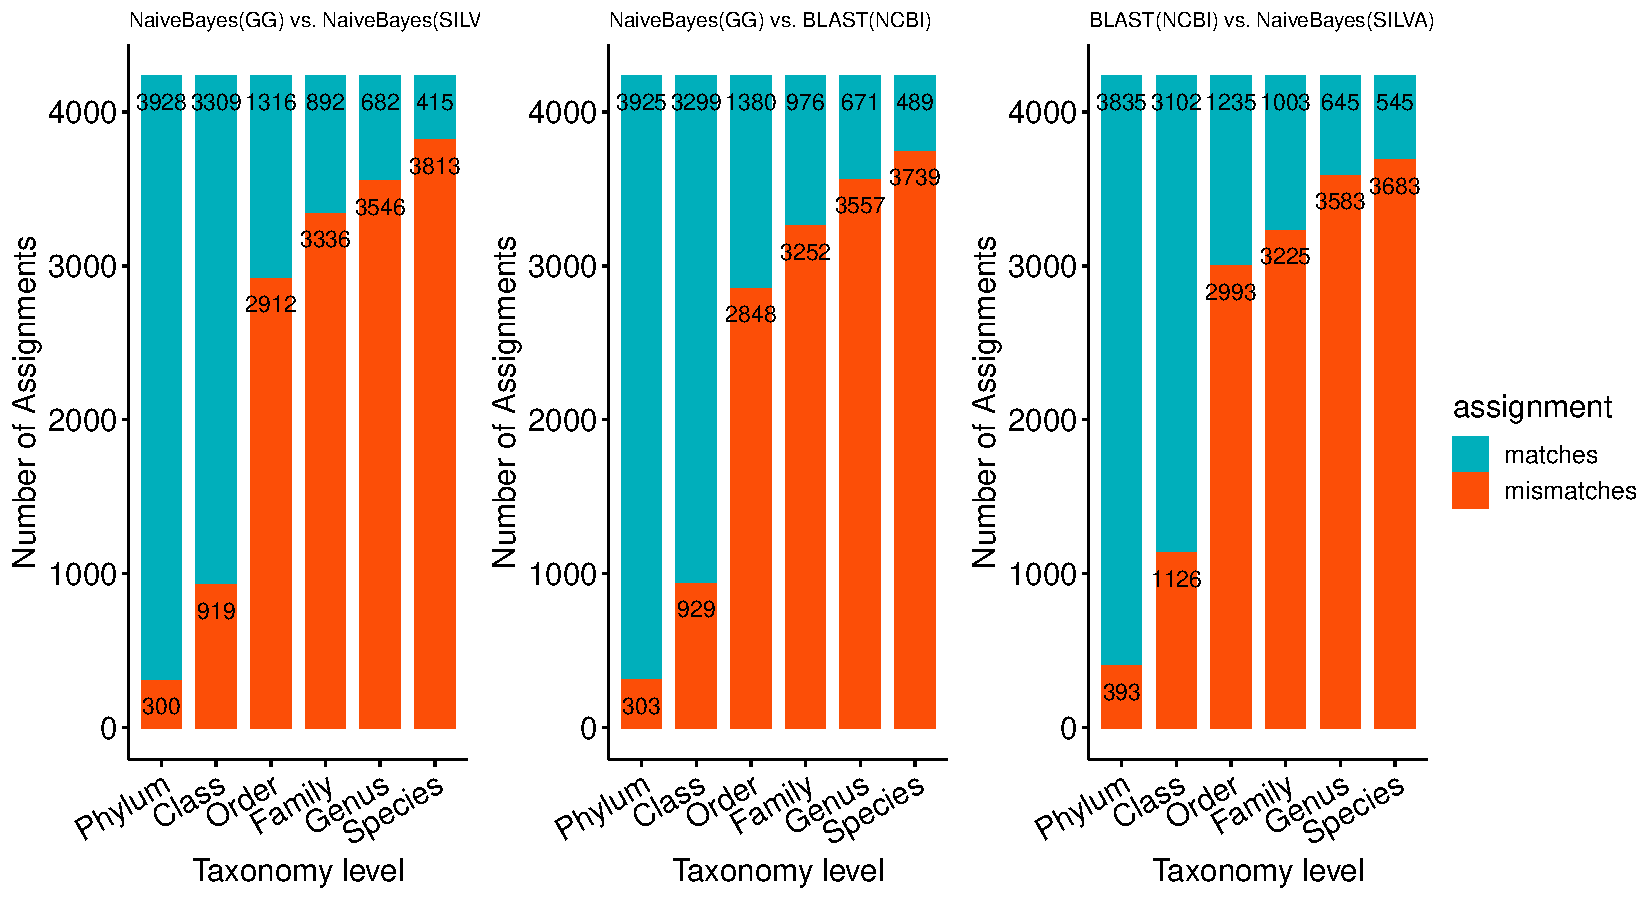
\includegraphics[width=1.0\linewidth]{figure_s4.pdf}
    % \end{figure}
    \begin{figure}[H]
      \centering
        \caption{
          \textbf{The pairwise comparison of assignments generated using different databases for all representative sequences has a higher proportion of mismatches}.
          The comparison made here is similar to Figure~\ref{fig:figure3}B, but instead of the top 100 taxonomic entities (by abundance), all the assignments from one database are matched with those from the other two databases.
          The higher percentage of mismatches implies that the assigned taxonomies in the more abundant sequences (top 100) match more consistently.
        }
      \label{fig:figure_s4}
    \end{figure}
    % \FloatBarrier
    % \newpage

  % \begin{figure}[H]
  %   \centering
  %   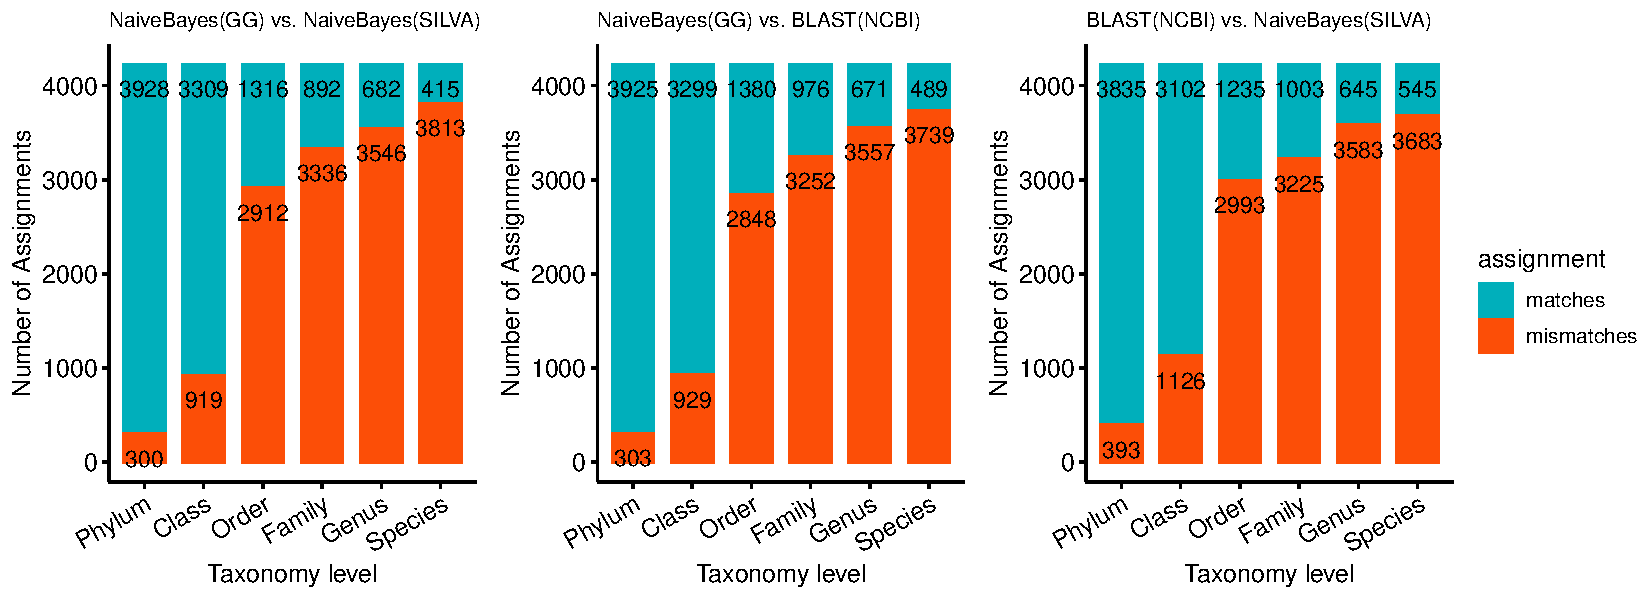
\includegraphics[width=1.0\linewidth]{figure_s5.pdf}
  % \end{figure}
  \begin{figure}[H]
    \centering
      \caption{
        \textbf{The precision and sensitivity of the inferred networks on the ``NorTA'' synthetic interaction data}.
        The different consensus methods used are scaled-sum (SS) and simple voting (SV) methods.
        Pearson and Spearman methods are not used in the calculation of the consensus.
        Among all the independent network inference methods, \acs{spieceasi} has the best average precision (0.944), but the overall best precision was consistently obtained by the scaled-sum method (0.956, 0.985, and 1.000).
        The simple voting method when using the presence of edges in all inferred networks as a requirement ($\theta = 1.000$), also outperforms \acs{spieceasi} on average precision (0.969).
        Although \acs{spieceasi} has a higher sensitivity, if the goal of network inference is to obtain the list of associations that have a high probability of existing in the real microbial community, then the consensus methods perform better.
      }
    \label{fig:figure_s5}
  \end{figure}
  % \FloatBarrier
  % \newpage

  % \begin{figure}[H]
  %   \centering
  %   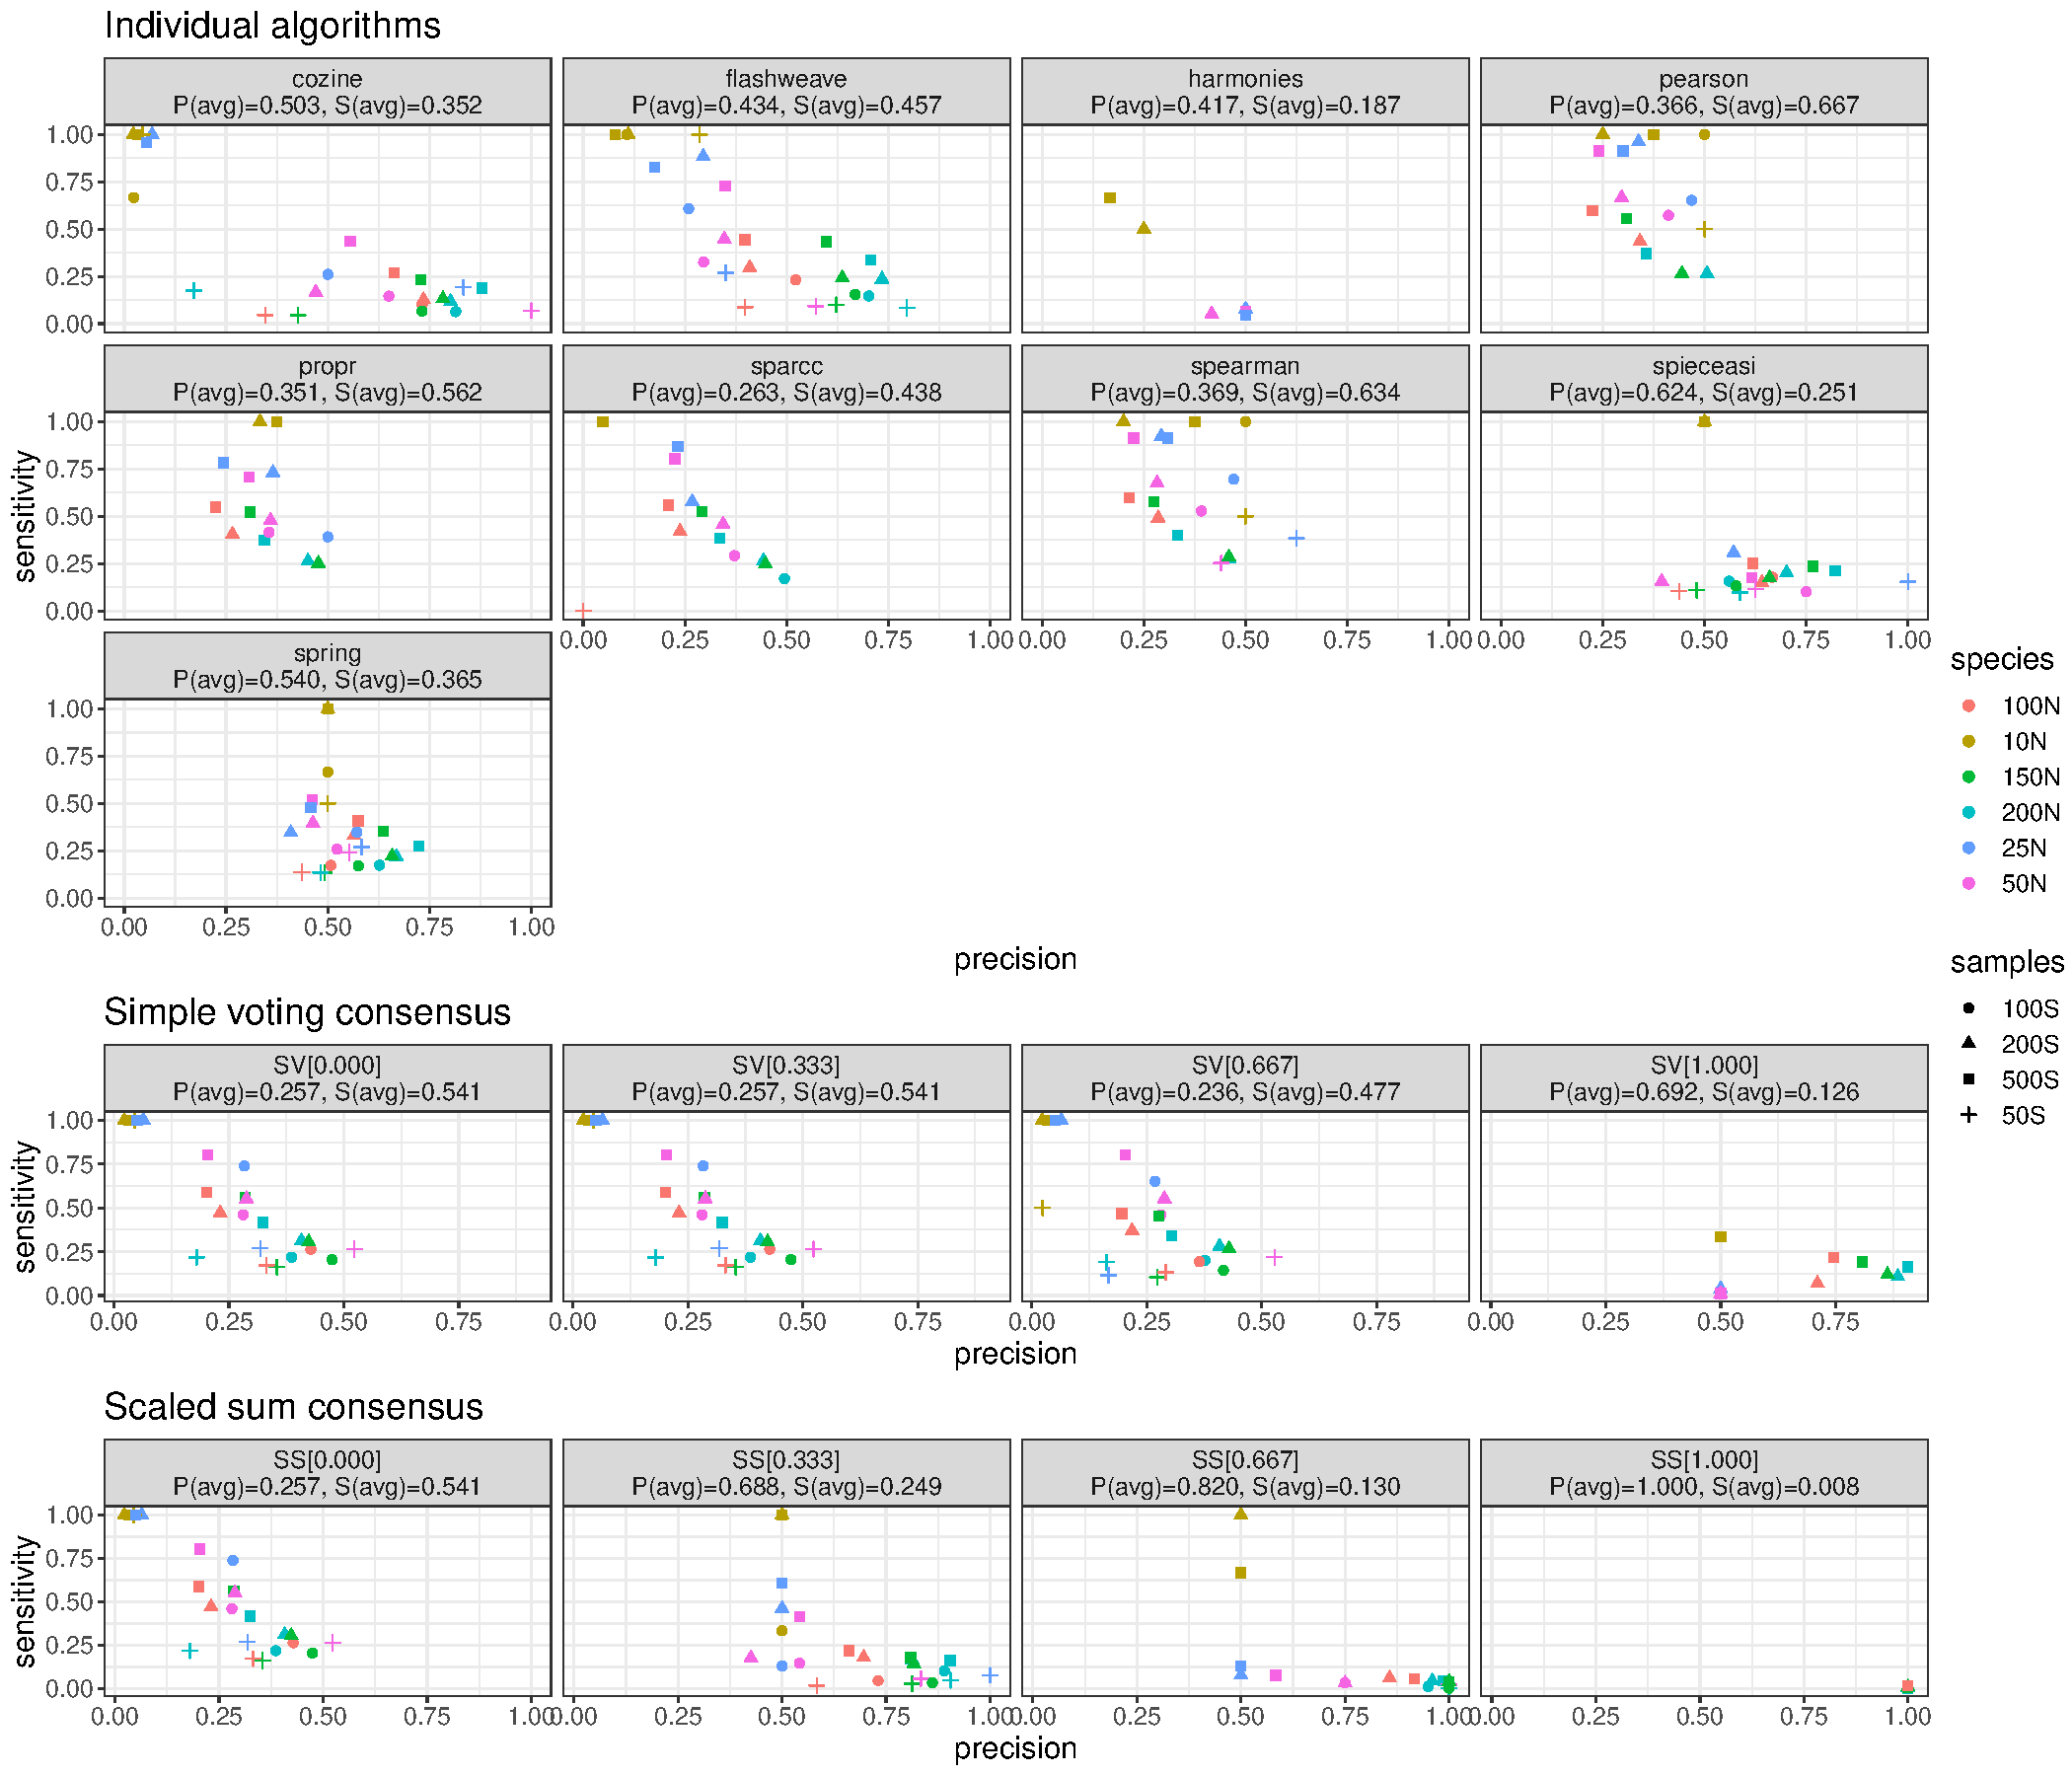
\includegraphics[width=1.0\linewidth]{figure_s6.pdf}
  % \end{figure}
  \begin{figure}[H]
    \centering
      \caption{
        \textbf{The precision and sensitivity of the inferred networks on the ``seqtime'' synthetic interaction data.}
        The different consensus methods used are scaled-sum (SS) and simple voting (SV) methods.
        Pearson and Spearman methods are not used in the calculation of the consensus.
        Among all the independent network inference methods, \acs{spieceasi} has the best average precision (0.624), but the overall best precision was consistently obtained by the scaled-sum method (0.688, 0.820, and 1.000).
        The simple voting method when using the presence of edges in all inferred networks as a requirement ($\theta = 1.000$), also outperforms \acs{spieceasi} on average precision (0.692).
        These results show that the scaled-sum method is not only much better suited for inferring robust and accurate interactions from count data generated from network topologies (NorTA), but it is also capable of accurately extracting real associations from Lotka-Volterra simulations.
      }
    \label{fig:figure_s6}
  \end{figure}
  % \FloatBarrier
  % \newpage

  % \begin{figure}[H]
  %   \centering
  %   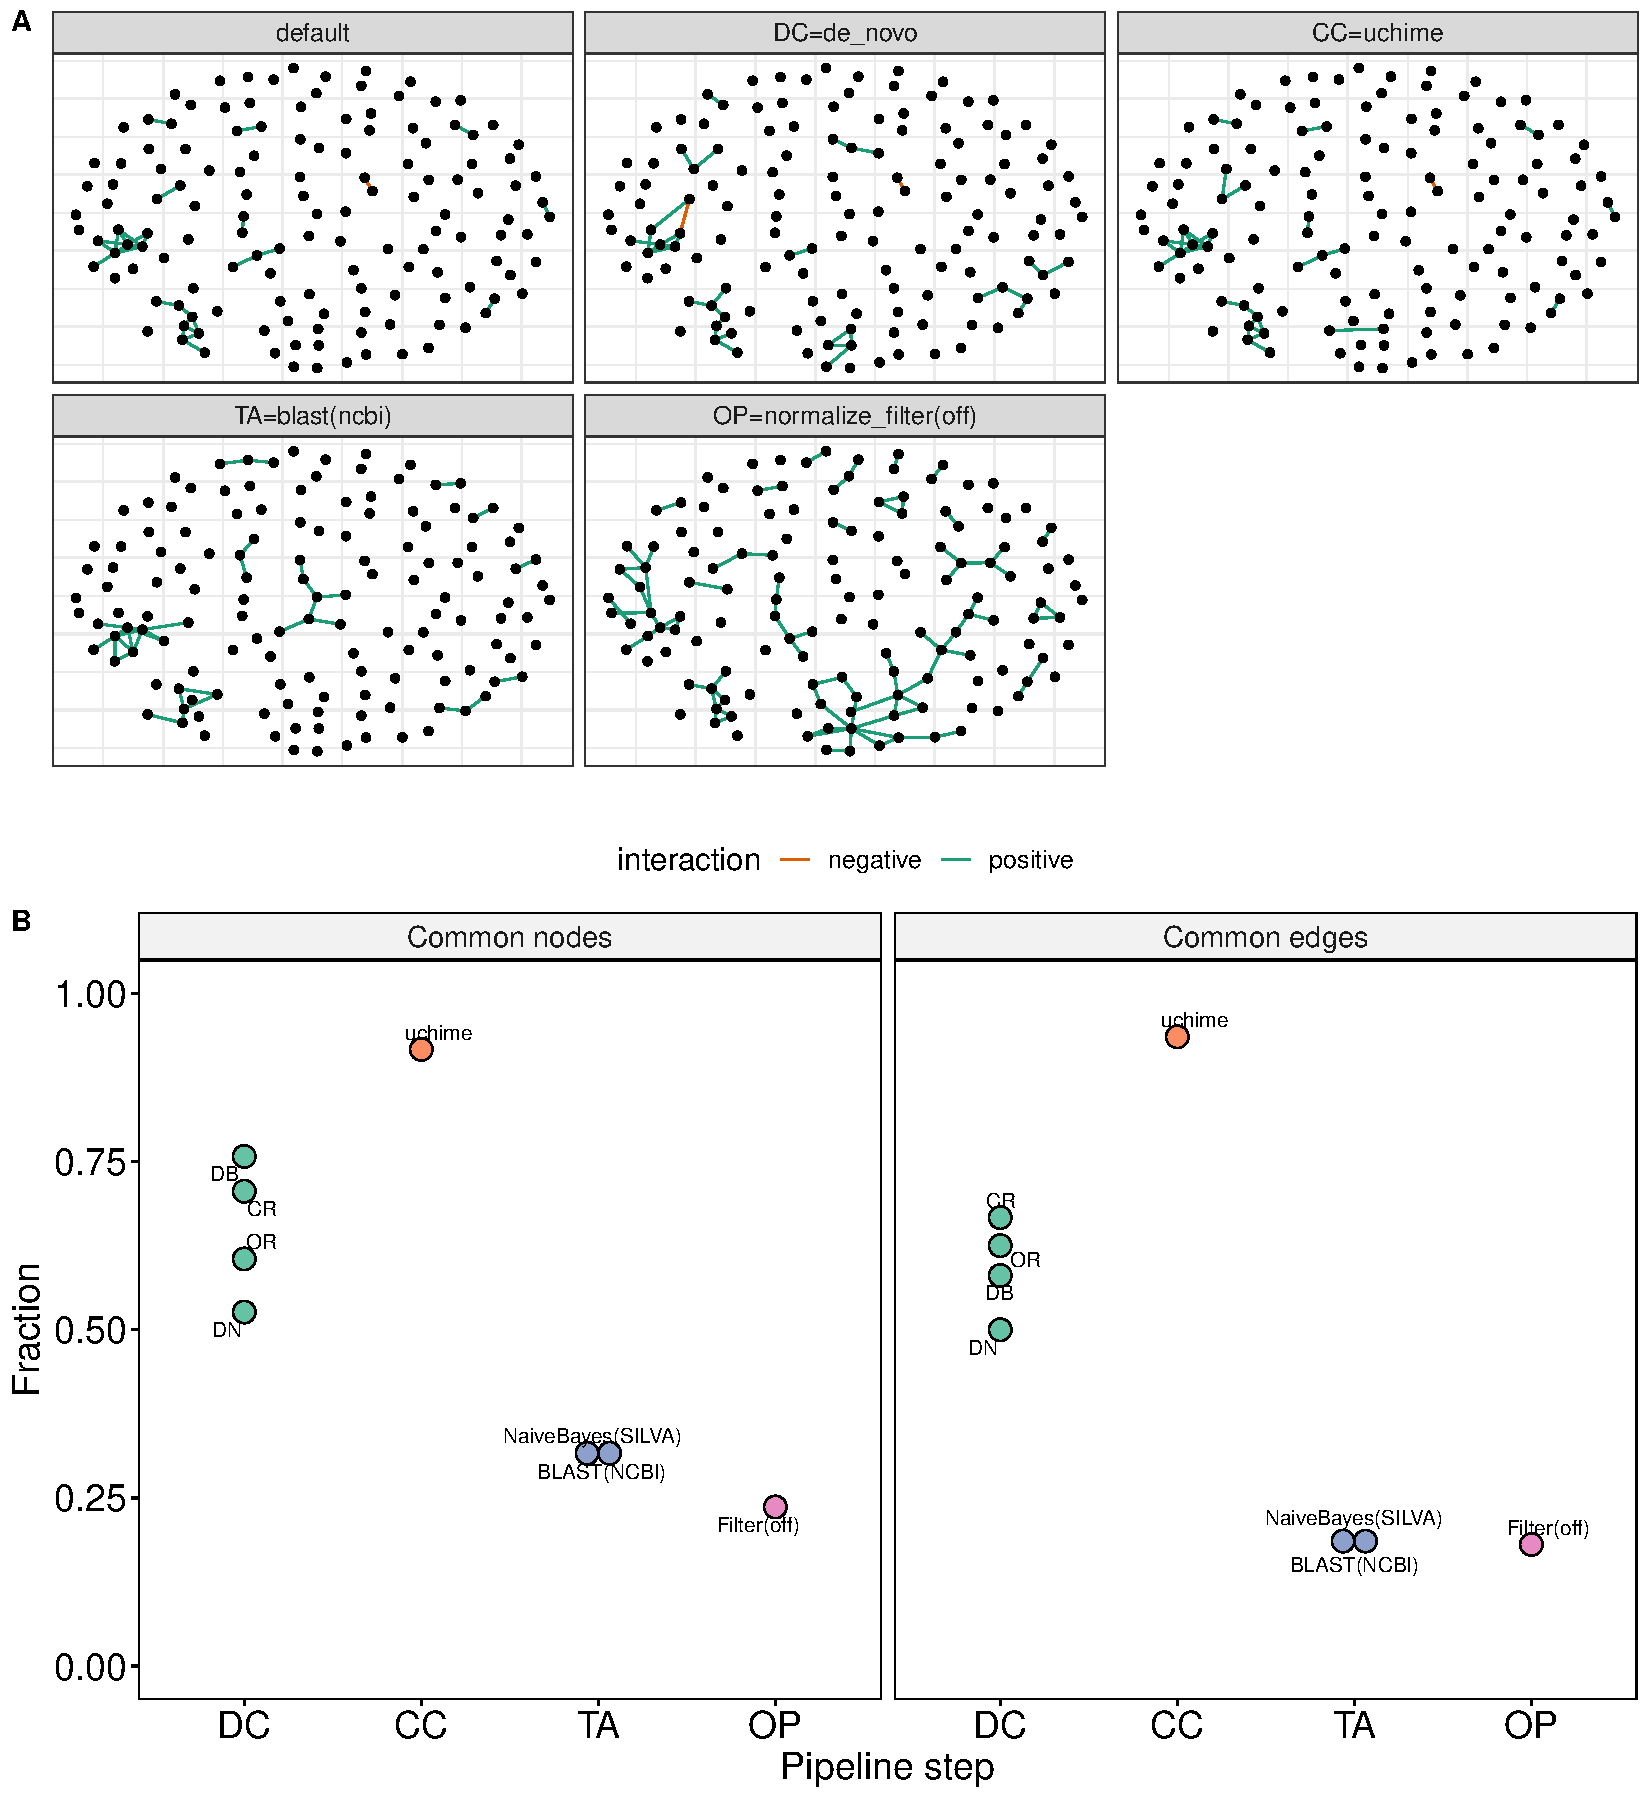
\includegraphics[width=1.0\linewidth]{figure_s7.pdf}
  % \end{figure}
  \begin{figure}[H]
    \centering
    \caption{
      \textbf{Sensitivity analysis of the default settings of the \ac{micone} pipeline}.
      \textbf{(A)} The network constructed using the default pipeline parameters (DC=\ac{dada2}, CC=remove bimera, TA=\ac{gg}, OP=Filter(on), NI=scaled-sum consensus) is compared against networks generated when one of the steps uses a different tool.
      The layout is created by fixing the positions of all the nodes from all networks and then drawing only the relevant edges, making the connections directly comparable.
      The edges colored green are positive associations and those in red are negative associations.
      We observe that changing the TA and OP steps leads to the creation of the most number of unique edges.
      \textbf{(B)} The dot plot showing the fraction of nodes (left) and edges (right) in common between the default network and the networks generated by changing one step of the default pipeline.
      The low value of the common fraction for TA and OP steps shows that these steps induce the biggest changes in nodes and edges.
      The NI step is not shown in this analysis because the consensus methods use edges from the individual network inference methods and a comparison would be biased.
    }
    \label{fig:figure_s7}
  \end{figure}
  % \FloatBarrier
  % \newpage

  \setcounter{figure}{0}
  \renewcommand{\figurename}{Text}
  \renewcommand{\thefigure}{S\arabic{figure}}
  \begin{figure}[H]
    \centering
    \caption{Supplemental text describing data processing, synthetic interaction data generation, network metrics, p-value merging and supplementary discussion sections.}
    \label{txt:text_s1}
  \end{figure}

\newpage
\section*{Supplementary Text}

  \subsection*{Processing the FMT data}

    \subsubsection*{Data download and pre-processing}
    The main biological dataset used in this study was the collection of 16S rRNA sequencing reads from stool samples (healthy and autistic individuals) for a fecal microbiome transplant study~\cite{Kang2017}.
    The data containing the 16S sequencing reads (V4 region) was downloaded from Qiita~\cite{gonzalezQiitaRapidWebenabled2018} (study ID: 10532).
    Only runs 2, 3, and 4 were used for the subsequent analysis as these runs consisted of paired-end sequencing data, and run 1 contained single-end data.
    The sample metadata was updated to contain only BMI, sex, height, weight, and experimental group.
    This was necessary as two of the network inference algorithms (\acs{mldm} and FlashWeave) required information about environmental heterogeneity.
    However, these environmental correlations were not included in the current analyses.

    \subsubsection*{Processing using the \ac{micone} pipeline}
    The data was then processed using the \ac{micone} pipeline starting at the \ac{sp} step and ending at the \ac{ni} step with the consensus algorithm.
    The configuration files (main.nf and nextflow.config) used to run the \ac{micone} pipeline as well the details of the pipeline execution (dag, report, timeline and trace) are in the "runs/FMT" directory of the data and scripts repository (\href{https://github.com/segrelab/MiCoNE-pipeline-paper}{https://github.com/segrelab/MiCoNE-pipeline-paper})
    The results of the pipeline execution for reproducing the analyses in the manuscript are stored on Zenodo.

  \subsection*{Processing the mock data}

    \subsubsection*{Data download and pre-processing}
    The mock datasets, mock4, mock12 and mock16 used for this study, were obtained from mockrobiota~\cite{Bokulich2016}.
    Mock 4 is a mock community composed of 21 bacterial strains represented in equal abundances in two replicate samples, and the same strains represented in uneven abundances in two other replicate samples.
    Mock 12 is composed of 27 bacterial strains containing closely related taxa, the members of which were chosen in part for their well-separated 16S rRNA gene sequences. Some pairs of strains differ by as little as one nucleotide, but all the strains are distinguishable over the sequenced region of the 16S rRNA gene.
    Mock 16 is a mock community composed of even amounts of purified genomic DNA from 49 bacteria and 10 archaea.
    The datasets did not require any preprocessing and could be directly used as input to the pipeline

    \subsubsection*{Processing using the \ac{micone} pipeline}
    The data was processed using the \ac{micone} pipeline starting at the \ac{sp} step and ending at the \ac{op} step with the filtered taxonomic tables as the final output.
    The configuration files (main.nf and nextflow.config) used to run the \ac{micone} pipeline as well the details of the pipeline execution (dag, report, timeline and trace) are in the "runs/mock*" directory of the data and scripts repository (\href{https://github.com/segrelab/MiCoNE-pipeline-paper}{https://github.com/segrelab/MiCoNE-pipeline-paper})
    The results of the pipeline execution for reproducing the analyses in the manuscript are stored on Zenodo.

    \subsubsection*{Interpretation of Unifrac results in the DC step}
  In Figure \ref{fig:figure_s3}, we observe that both the weighted and unweighted UniFrac distances are increased for the top 1000 representative sequences, implying that the top representative sequences generated by the different methods are not as similar to each other.
  Therefore, since the weighted UniFrac distances are lower than the unweighted distances, we conclude that the representative sequences in the middle range of the abundance distribution are those that must be the most similar between the methods.

    Open-reference and de novo clustering methods perform the best under the weighted UniFrac metric and the worst (marginally) under the unweighted UniFrac metric (Figure~\ref{fig:figure2}C and \ref{fig:figure2}D).
    This result can be attributed to the large number of low abundance representative sequences that are generated by these methods.
    Deblur performs poorly under weighted Unifrac and although its performance on the mock4 dataset is the best under unweighted UniFrac, its performance on the other datasets is average.
    The Deblur method returns a very small number of representative sequences (2388) and this could account for the reason for the high dissimilarity with the other methods as well as irregular performance on the mock data.

  \subsection*{Synthetic interaction data}

    \subsubsection*{Data generation}
    The synthetic interaction data for the study were generated using two methods.
    The first method, ``seqtime''~\cite{faustSignaturesEcologicalProcesses2018} utilized generalized Lotka-Volterra (gLV) equations to model the microbial community dynamics and made use of the Klemm–Eguı́luz algorithm to generate clique-based interaction networks~\cite{Rottjers2018}.
    We used the seqtime R package to simulate communities with different numbers of species and samples (see Methods for details).
    The second method, ``NorTA'' used the Normal to Anything (NorTA) approach coupled with a given interaction network topology to generate the abundance distribution of the microbial community~\cite{Kurtz2015}.
    We used the spieceasi R package to simulate communities with different abundance distributions and network topologies (see Methods for details).
    The scripts to generate these datasets can be found in the synthetic data and scripts repository (\href{https://github.com/segrelab/MiCoNE-synthetic-data}{https://github.com/segrelab/MiCoNE-synthetic-data})

    \subsubsection*{Processing using the \ac{micone} pipeline}
    The data was processed using the \ac{micone} pipeline using only the \ac{ni} step with the consensus networks as the final output.
    The configuration files (main.nf and nextflow.config) used to run the \ac{micone} pipeline as well the details of the pipeline execution (dag, report, timeline and trace) are in the "runs/norta" and "runs/seqtime" directories of the data and scripts repository (\href{https://github.com/segrelab/MiCoNE-pipeline-paper}{https://github.com/segrelab/MiCoNE-pipeline-paper})
    The results of the pipeline execution for reproducing the analyses in the manuscript are stored on Zenodo.


  \subsection*{Network metrics}

  In Table~\ref{tab:network_metrics} we show various global network metrics calculated for each tool in the pipeline.
  %\todo[noline]{R2.1a}
  %\todo[noline]{R2.7}
  All the networks that make use of a particular tool are grouped together, and the following average metrics are calculated for each group:
  \begin{enumerate}
    \item The average shortest path length describes the average of all the shortest paths in the graph. No number is reported if the graph is not connected, therefore, the results indicate that none of the networks that make use of \acs{harmonies}, \acs{cozine}, \acs{spring}, \acs{spieceasi} and Pearson are connected.
    \item The average clustering is the average clustering coefficient of the graph. The closer the value is to 1.0, the more densely connected is the graph. We can observe that the networks that use correlation-based methods have the highest values while the direct association based methods have the lowest.
    \item The number of connected components is the highest for the direct association based methods and the lowest for the correlation-based methods. In the case of propr, all the networks have only one giant component.
    \item The modularity metric is the modularity over all partitions in a graph calculated using a label propagation algorithm~\cite{cordascoCommunityDetectionSemisynchronous2010}. Positive values imply that there are more edges between vertices of the same type than we would expect by chance, and negative implies that there are less. The networks inferred by \acs{mldm} report very few edges, and skew the average modularity scores. This could also be an artifact of incomplete convergence of the \acs{mldm} algorithm for some combinations.
    \item Node connectivity refers to the minimum number of nodes that must be removed from the graph to make it disconnected. We observe that only the networks generated using propr have a high value since most of these networks are connected.
    \item Degree assortativity coefficient measures the similarity of connections in the graph with respect to the node degree. Again we observe that the direct association based methods have a negative degree of assortativity, meaning that there are many hubs in these networks. The correlation-based methods have positive values implying that in these networks nodes with similar degrees attach to one another.
  \end{enumerate}
  A weight threshold of 0.1 and a p-value threshold of 0.05 were applied to each network before the analysis.
  All the metrics were calculated using the \texttt{networkx} Python package~\cite{hagbergExploringNetworkStructure2008}.

  \subsection*{p-value merging}

  Fisher~\cite{fisher_224a_1948} proposed that for $k$ independent p-values, each generated by $k$ different methods and denoted by $\bar{P}^i$ (notations are same as used in the "Consensus network and p-value merging" subsection of the Methods).
  %\todo[noline]{R1.1}
  The following will hold true for the statistic $\Psi$:
  \begin{equation*}
    \begin{aligned}
      \Psi &= \sum_{i=1}^k -2 \log \left( \bar{P}^i \right) \\
        \Psi &\sim \chi^2_{2k}
    \end{aligned}
  \end{equation*}

  Brown~\cite{brown_400_1975} extended Fisher's method to dependent p-values by using a re-scaled $\chi^2$ distribution:
  \begin{equation*}
    \Psi \sim c \chi^2_{2f}
  \end{equation*}
  where, $f$ is the degrees of freedom and $c$ is the scale factor and are given by:
  \begin{equation*}
    f = \frac{\mathrm{E}[\Psi]^2}{\mathrm{Var}[\Psi]} ~~~\text{and}~~~ c = \frac{\mathrm{Var}[\Psi]}{2\mathrm{E}[\Psi]} = \frac{k}{f}
  \end{equation*}

  We can calculate $E[\Psi]$ and $Var[\Psi]$ under the null hypothesis that the data are drawn from a multivariate Gaussian with some covariance matrix.
  We then use these values to parametrize a $\chi^2$ distribution from which the p-value corresponding to $\frac{\psi}{c}$ can be calculated.
  Furthermore, Brown showed that $\mathrm{E}[\Psi]$ and $\mathrm{Var}[\Psi]$ can be calculated via the following numerical approximation:
  \begin{equation*}
    \mathrm{E}[\Psi] = 2k ~~~\text{and}~~~ \mathrm{Var}[\Psi] = 4k + 2\sum_{i<j} \mathrm{Cov}\left( -2\log(\bar{P}^i), -2\log(\bar{P}^j) \right)
  \end{equation*}

  The above formulation was improved by Kost and McDermott~\cite{kost_combining_2002} by further fitting a third-order polynomial to approximate the covariance
  \begin{equation}
    \mathrm{Cov}\left( -2\log(\bar{P}^i), -2\log(\bar{P}^j) \right) \approx 3.263 \rho_{ij} + 0.710 \rho_{ij}^2 + 0.027 \rho_{ij}^3
    \label{eqn:suppl_covariance-pvalues}
  \end{equation}
  where, $\rho_{ij}$ is the correlation between method $i$ and method $j$

  Using $E[\Psi]$ and $Var[\Psi]$ we then fit a $\chi^2$ distribution with the parameters $c$ and $f$.
  Note that since, in general, $f$ will not be an integer, this should be understood as a Gamma distribution with a shape parameter $f$, as mentioned by Brown~\cite{brown_400_1975}.
  Using this, we calculate the test $\psi$ and compute the p-value from the CDF of the $\chi^2$ distribution, given in Equation~\ref{eqn:suppl_pvalue-combined}.
  Therefore, the final combined p-value~\cite{Poole_Gibbs_Shmulevich_Bernard_Knijnenburg_2016} is then given by:
  \begin{equation}
    \begin{aligned*}
        & \hat{P}_j = 1.0 - \Phi_{2f}\left( \psi / c \right) \\
        \text{where},~ &\psi = -2 \sum_{i=1}^k \log(\bar{P}^i_j) ~~~\text{and}~~~ \Phi_{2f} = \mathrm{CDF}\left( \chi^2_{2f} \right)
    \end{aligned*}
    \label{eqn:suppl_pvalue-combined}
  \end{equation}

  The p-value merging and consensus method in \ac{micone} (see Methods) uses Equation~\ref{eqn:suppl_covariance-pvalues} to estimate the covariance of the p-values and Equation~\ref{eqn:suppl_pvalue-combined} to merge the p-values (obtained from bootstrapping) from the different correlation methods.
  Note that we do not use Pearson and Spearman methods in the p-value merging step and these algorithms are only used for demonstration and comparison.
  The combined p-values are used to threshold for significance in the correlation-based networks during the consensus network step.

  \subsection*{The JSON network format and network exports}

    The default format \ac{micone} uses for storing the network files is the JSON (JavaScript Object Notation) format which is supported by the \acf{mind}~\cite{huResourceComparisonIntegration2022}.
    The custom JSON schema we have designed is able to store all network-related information pertaining to nodes, links, and the metadata related to the links and datasets.
    Additionally, \ac{micone} also supports exporting of networks into a variety of other formats such as edge lists, GML, and Cytoscape formats.
    Since we make use of \texttt{networkx}~\cite{hagbergExploringNetworkStructure2008} for the export functionality, networks can be exported to all formats supported by the package.
    However, not all the corresponding metadata will be exported appropriately, as most formats do not support this additional metadata.
    The details of the format and information about importing/exporting it and other network formats can be found in the \ac{micone} documentation.

  \subsection*{Supplementary discussion}

  It is worth pointing out some additional, more specific, conclusions stemming from the individual steps of our analysis.
  The different denoising/clustering methods differ mostly in their identification of sequences that are in low abundance.
  Hence, they do not have much of an impact on the inferred co-occurrence networks when the sequences of low abundance are removed (Figure~\ref{fig:figure1}).
  Comparison of inferred and expected reference sequences and their abundances in mock community datasets has allowed us to identify \ac{dada2} as the method which best recapitulates the expected sequence composition.
  For the chimera checking module, we suggest using the remove bimera method since it was developed in conjunction with \ac{dada2} and its performance does not significantly differ from uchime-denovo.
  For the current work, we have decided to focus on the tools most widely used at the time of the analysis.
  Some tools which were not as widely used (e.g. dbOTU3~\cite{Olesen2017}) as well as older popular methods like mothur~\cite{Schloss2009} have not been included in the study but could be added into the pipelines in future updated analyses.

  The choice of taxonomy database was found to be the most important factor in the inference of microbial co-occurrence networks, contributing $65.4\%$ of the total variance.
  %\todo[noline]{R2.2a}
  The frequent changes in the taxonomy nomenclature coupled with the frequency of updates to the various 16S reference databases create inherent differences \cite{Balvociute2017} in taxonomy hierarchies in these databases.
  Our analysis revealed that no particular reference database performs better than the others across the different mock dataset benchmarks.
  %\todo[noline]{R2.12}
  The default reference database in the pipeline is the \ac{gg} reference database along with the ``Naive Bayes'' classifier as the query tool.
  The reason for our choice stems from the popularity of the \ac{gg} database~\cite{parkEvaluation16SRRNA2018} in taxonomic studies, which would enable easy comparison across datasets.
  However, for newer studies we recommend using SILVA database because of its size and taxonomic comprehensiveness~\cite{iiRESCRIPtReproducibleSequence2021} and since \ac{gg} has not been updated since 2013.
  Additionally, a particular database might be more appropriate than the rest based on specific requirements.
  For example, to generate a dataset that is compatible with the \ac{mind} platform~\cite{huResourceComparisonIntegration2022} \ac{ncbi} is the most appropriate choice as it guarantees compatibility of taxonomic hierarchy and therefore comparability with other datasets.
  Furthermore, we also enable users to use custom databases~\cite{Ritari2015,iiRESCRIPtReproducibleSequence2021} with the BLAST and Naive Bayes classifiers that are incorporated into the pipeline (from \ac{qiime2}).
  We suggest that the choice of the database should be made based on possible reported or inferred biases in the representation of given biomes in a specific databases~\cite{Balvociute2017,iiRESCRIPtReproducibleSequence2021}, as choosing taxon-specific databases have also been observed to compromise classification~\cite{rmarcelinoUseTaxonspecificReference2020}.

  The \ac{op} step of the pipeline is second in its contribution to total network variance.
  This can be attributed to the large number of nodes that are added to the final networks when the filtering is turned off.
  Additionally, a very large number of nodes also decreases the accuracy of the network inference algorithms for the same sample size~\cite{peschelNetCoMiNetworkConstruction2020} and increases the computational complexity~\cite{tackmannRapidInferenceDirect2019}.
  We observe that filtering out taxa that are present in low abundances in all samples increases the proportion of taxa in common between taxonomy tables generated using different reference databases (Figure~\ref{fig:figure_s4}), providing another reason for filtering.
  We also observe that the reduction in the number of taxa leads to a better agreement in the networks inferred through different methods (Figure~\ref{fig:figure6} and Figure~\ref{fig:figures1}).
  Moreover, filtering is necessary in order to increase the power in tests of significance when the number of taxa is much greater than the number of samples.

\newpage
  \pagenumbering{goggle}
  \thispagestyle{empty}
    \begin{table}[H]
    \centering
    \begin{tabular}{|c|c|c|c|}
      \hline
      \textbf{Workflow step} & \textbf{Module/Condition} & \textbf{Tool/Parameter} & \textbf{References/Value} \\
      \hline
      \multirow{7}{*}{Denoising and Clustering} & \multirow{5}{*}{Denoise and Cluster} & Closed reference & \cite{rognesVSEARCHVersatileOpen2016,bolyenReproducibleInteractiveScalable2019} \\
                                                &  & Open reference & \cite{rognesVSEARCHVersatileOpen2016,bolyenReproducibleInteractiveScalable2019} \\
                                                &  & De novo & \cite{rognesVSEARCHVersatileOpen2016,bolyenReproducibleInteractiveScalable2019} \\
                                                &  & \rowcolor{lightgray} Dada2 & \cite{Callahan2016} \\
                                                &  & Deblur & \cite{Amir2017,bolyenReproducibleInteractiveScalable2019} \\
                                                \cline{2-4}
                                                & \multirow{2}{*}{Chimera checking} & Uchime-denovo & \cite{rognesVSEARCHVersatileOpen2016,bolyenReproducibleInteractiveScalable2019} \\
                                                & & \rowcolor{lightgray} Remove bimera & \cite{Callahan2016} \\
                                                \hline
      \multirow{5}{*}{Taxonomy assignment} &  \multirow{2}{*}{Query tool} & Blast & \cite{camachoBLASTArchitectureApplications2009,bokulichOptimizingTaxonomicClassification2018} \\
                                           &  & \rowcolor{lightgray} Naive bayes classifier & \cite{bokulichOptimizingTaxonomicClassification2018} \\
                                           \cline{2-4}
                                           & \multirow{3}{*}{Database} & \rowcolor{lightgray} Greengenes 13\_8 & \cite{DeSantis2006} \\
                                           & & SILVA 138 & \cite{Quast2012} \\
                                           & & NCBI RefSeq (Oct 2021) & \cite{Sayers2009} \\
      \hline
      \multirow{6}{*}{OTU processing} & \multirow{3}{*}{Filter(off)} & Prevalence threshold      & 2 / n\_samples \\
                                      & & Abundance threshold       & 0.001          \\
                                      & & Observation sum threshold & 10             \\ \cline{2-4}
                                      & \multirow{3}{*}{Filter(on)}  & \rowcolor{lightgray} Prevalence threshold      & 0.05           \\
                                      & & \rowcolor{lightgray} Abundance threshold       & 0.01           \\
                                      & & \rowcolor{lightgray} Observation sum threshold & 100            \\
      \hline
      \multirow{12}{*}{Network Inference} & \multirow{2}{*}{Bootstrapping}& fastspar\_bootstraps v1.0 & \cite{Watts2018} \\
                                          & & fastspar\_pvalues v1.0 & \cite{Watts2018} \\
                                          \cline{2-4}
                                          & \multirow{6}{*}{Direct association} & \ac{spieceasi} v1.1.2 & \cite{Kurtz2015} \\
                                          & & FlashWeave.jl v0.18.1 & \cite{tackmannRapidInferenceDirect2019} \\
                                          & & \ac{cozine} v1.0 & \cite{haCompositionalZeroinflatedNetwork2020a} \\
                                          & & \ac{harmonies} v1.0 & \cite{jiangHARMONIESHybridApproach2020} \\
                                          & & \ac{spring} v1.0.4 & \cite{yoonMicrobialNetworksSPRING2019} \\
                                          & & \ac{mldm} v1.1 & \cite{Yang2017} \\
                                          \cline{2-4}
                                          & \multirow{2}{*}{Correlation-based} & FastSpar (\ac{sparcc}) v1.0 & \cite{Watts2018} \\
                                          & & Pearson & - \\
                                          & & Spearman & - \\
                                          & & propr v2.1.2 & \cite{quinnProprRpackageIdentifying2017} \\ \cline{2-4}
                                          & \multirow{2}{*}{Consensus algorithm} & \rowcolor{lightgray} scaled-sum & 0.333 \\
                                          & & simple voting & 1.000 \\
      \hline
    \end{tabular}
  \end{table}

  \thispagestyle{empty}
  \begin{landscape}
\begin{table}[H]
  \centering
  \small
  \begin{tabular}{|l|p{1cm}|p{1cm}|p{1cm}|p{2cm}|p{1.5cm}|p{1.5cm}|p{1.5cm}|p{1.5cm}|p{1.5cm}|p{1.5cm}|p{1.5cm}|}
\hline
DC & CC            & TA                & OP          & NI         & Average shortest path length & Average clustering & No. of connected components & Modularity & Node connectivity & Degree assortativity coefficient \\ \hline
DB & -             & -                 & -           & -          & 2.066                        & 0.265              & 27.088                      & 0.387      & 1.868             & 0.070                            \\
OR & -             & -                 & -           & -          & 1.904                        & 0.273              & 24.868                      & -17.060    & 1.877             & 0.099                            \\
D2 & -             & -                 & -           & -          & 2.263                        & 0.267              & 28.228                      & 0.326      & 1.789             & 0.078                            \\
DN & -             & -                 & -           & -          & 2.065                        & 0.272              & 25.132                      & 0.302      & 1.754             & 0.093                            \\
CR & -             & -                 & -           & -          & 1.937                        & 0.276              & 24.289                      & -1.865     & 2.079             & 0.097                            \\
-  & remove bimera & -                 & -           & -          & 2.070                        & 0.272              & 25.968                      & -7.439     & 1.863             & 0.086                            \\
-  & uchime        & -                 & -           & -          & 2.066                        & 0.269              & 25.874                      & 0.275      & 1.884             & 0.089                            \\
-  & -             & NCBI              & -           & -          & 2.218                        & 0.262              & 22.784                      & -3.683     & 1.495             & 0.100                            \\
-  & -             & SILVA             & -           & -          & 1.872                        & 0.275              & 30.716                      & 0.415      & 2.674             & 0.074                            \\
-  & -             & GG                & -           & -          & 2.086                        & 0.274              & 24.263                      & -7.478     & 1.453             & 0.088                            \\
-  & -             & -                 & On          & -          & 1.975                        & 0.252              & 18.493                      & -7.194     & 1.880             & 0.073                            \\
-  & -             & -                 & Off         & -          & 2.193                        & 0.291              & 34.174                      & 0.431      & 1.867             & 0.104                            \\
-  & -             & -                 & -           & propr      & 1.650                        & 0.528              & 1.000                       & 0.000      & 10.583            & 0.036                            \\
-  & -             & -                 & -           & harmonies  &                              & 0.108              & 82.633                      & 0.757      & 0.000             & 0.340                            \\
-  & -             & -                 & -           & flashweave & 3.878                        & 0.079              & 1.800                       & 0.458      & 0.383             & -0.032                           \\
-  & -             & -                 & -           & cozine     &                              & 0.090              & 82.167                      & 0.694      & 0.000             & -0.072                           \\
-  & -             & -                 & -           & spring     &                              & 0.092              & 11.767                      & 0.566      & 0.000             & -0.035                           \\
-  & -             & -                 & -           & sparcc     & 1.747                        & 0.525              & 1.033                       & 0.009      & 5.500             & -0.011                           \\
-  & -             & -                 & -           & spieceasi  &                              & 0.076              & 39.383                      & 0.717      & 0.000             & -0.031                           \\
-  & -             & -                 & -           & pearson    &                              & 0.457              & 23.883                      & 0.551      & 0.000             & 0.478                            \\
-  & -             & -                 & -           & spearman   & 1.875                        & 0.551              & 1.450                       & 0.044      & 1.117             & 0.170                            \\
-  & -             & -                 & -           & mldm       & 2.760                        & 0.130              & 2.267                       & -75.648    & 0.433             & -0.028                           \\ \hline
\end{tabular}
\end{table}
\end{landscape}


%--------------------------------------------------------%
%   END DOCUMENT
%--------------------------------------------------------%

\end{document}
